%------------------------------------------------------------------------------
% SMURF Paper
%------------------------------------------------------------------------------

\documentclass[useAMS,usenatbib,nofootinbib]{mn2e}

%% Recommended by MN for handling hyperlinks
\usepackage[pdftex,pdfpagemode={UseOutlines},bookmarks,bookmarksopen,colorlinks,linkcolor={blue},citecolor={green},urlcolor={red}]{hyperref}

% this is needed to get pdftex to work properly!
\usepackage[pdftex]{graphicx}

\usepackage{amsmath}
\usepackage{url}
\usepackage{natbib}
\usepackage{rotating}

% --- Some user defined macros ------------------------------------------------

% journals
\newcommand{\ao}{AO}
\newcommand{\apj}{ApJ}
\newcommand{\apjl}{ApJL}
\newcommand{\apjs}{ApJS}
\newcommand{\aaps}{A$\&$AS}
\newcommand{\aap}{A$\&$A}
\newcommand{\aapr}{A$\&$AR}
\newcommand{\mnras}{MNRAS}
\newcommand{\aj}{A J}
\newcommand{\araa}{\rm ARA\&A}
\newcommand{\nat}{Nat}
\newcommand{\pasj}{PASJ}
\newcommand{\pasp}{PASP}
\newcommand{\prd}{PhRvD}
\newcommand{\ASP}{ASP Conf.\ Ser.~}
\newcommand{\CASP}{\rm Comm. Astrophys. Space Phys.}
\newcommand{\astroph}{\rm astro-ph/}
\newcommand{\spie}{Proc.\ SPIE~}


% common acronyms etc.
\newcommand{\snr}{SNR}
\newcommand{\scuba}{SCUBA-2}
\newcommand{\rms}{RMS}

% these are approximately less-than and greater-than symbols
\def\lsim{\mathrel{\lower2.5pt\vbox{\lineskip=0pt\baselineskip=0pt
          \hbox{$<$}\hbox{$\sim$}}}}

\def\gsim{\mathrel{\lower2.5pt\vbox{\lineskip=0pt\baselineskip=0pt
          \hbox{$>$}\hbox{$\sim$}}}}

% sinc function
\def\sinc{\mathrm{sinc}}

% how are model names displayed
\newcommand{\model}[1]{\texttt{#1}}

% ----------------------------------------------------------------------------

\title[\scuba: iterative map-making with SMURF]{\scuba: iterative map-making
with the Sub-Millimetre User Reduction Facility}

\author[Edward~L.~Chapin~et~al.]{
  \parbox[t]{\textwidth}{
    Edward~L.~Chapin$^{1,2}$\thanks{E-mail:~echapin@sciops.esa.int,
      Present address: XMM SOC, ESAC, Apartado 78, 28691 Villanueva de
      la Ca\~nada, Madrid, Spain},
    David~S.~Berry$^{2}$,
    Andrew~G.~Gibb$^{1}$,
    Tim~Jenness$^{2}$,
    Douglas~Scott$^{1}$,
    Remo~P.~J.~Tilanus$^{2,3}$,
    Frossie~Economou$^2$\thanks{Present address: National Optical
      Astronomy Observatory, 950 N.\ Cherry Avenue, Tucson, AZ 85719, USA},
  }
  \\
  \\
  $^{1}$Dept. of Physics \& Astronomy, University of British Columbia,
  6224 Agricultural Road, Vancouver, B.C. V6T 1Z1, Canada\\
  $^{2}$JointAstronomy Centre, 660 N. A`oh\={o}k\={u} Place, University
  Park, Hilo, Hawaii 96720, USA\\
  $^{3}$Netherlands Organisation for Scientific Research,
  Laan van Nieuw Oost-Indie 300, NL-2509 AC The Hague, The Netherlands}
\begin{document}

\label{firstpage}

\maketitle

\begin{abstract}
  The Submillimetre Common User Bolometer Array 2 (\scuba) is an
  instrument operating on the 15-m James Clerk Maxwell Telescope,
  consisting of about 5000 bolometers in each of two simultaneous
  imaging bands centred over 450 and 850\,\micron. The camera is
  operated by scanning across the sky and records data at a rate of
  200\,Hz. The data rate is much greater than that of previously
  existing submillimetre cameras, and represents a significant
  analysis challenge. We describe the production of \scuba\ maps using
  the Sub-Millimetre User Reduction Facility (SMURF) in which we have
  adopted a fast, iterative approach to map-making that enables data
  reduction on single, modern, high-end desktop computers, with
  execution times that are shorter than the observing times.  SMURF is
  used in an automated setting, both at the telescope for real-time
  feedback to observers, as well as for the production of generic
  science products at the Canadian Astronomy Data Centre. A suite of
  tools is also provided for interactive data analysis.  Three
  detailed case studies are used to: (i) explore convergence
  properties of the map-maker using simple prior constraints (Uranus
  -- a point source); (ii) achieve the white-noise limit of the
  instrument for faint point-source studies (blank-field survey of the
  Lockman Hole); and (iii) demonstrate that our strategy is capable of
  recovering angular scales up to the size of the array footprint
  (approximately 5\,arcmin) for bright extended sources (star-forming
  region M17).
\end{abstract}


\begin{keywords}
methods: data analysis, techniques: image processing, submillimetre:
general, methods: observational
\end{keywords}

%------------------------------------------------------------------------------
\section{Introduction}
\label{sec:intro}
%------------------------------------------------------------------------------

The Submillimetre Common User Bolometer Array 2
\citep[\scuba,][]{holland2012} is a new instrument for the 15-m James
Clerk Maxwell Telescope (JCMT) on Mauna Kea, Hawai'i. The camera
simultaneously images the sky in two broad bands centred over 450 and
850\,\micron, with approximately 7.5 and 14.5\,arcsec full-width at
half-maximum (FWHM) point spread functions (PSFs). The focal planes at
each wavelength are populated with 4 rectangular subarrays, consisting
of $40 \times 32$ bolometers each, and together subtend a nearly
7\,arcmin $\times$ 7\,arcmin footprint on the sky (excluding gaps, the
continuous solid angle is about 43\,arcmin$^{2}$ per focal plane).
This paper describes the properties of \scuba\ data that are relevant
for producing maps of the imaging data, and the Submillimetre User
Reduction Facility, SMURF, a software package for performing the
reduction written using the Starlink Software Environment
\citep{1993ASPC...52..229W,2009ASPC..411..418J}. The details of the instrument design,
performance, and calibration are given in two companion papers:
\citet{holland2012} and \citet{dempsey2012}.

Over the last twenty years, observations in the submillimetre band
(defined here to be 200--1200\,\micron) have helped revolutionise
several important areas of astrophysics, including: the
characterisation of the early stages of star-formation by identifying
the dense, cold regions in molecular clouds where stars may eventually
form; discovering through blind surveys a class of massive dusty
star-forming galaxies in the early ($z>2$) Universe, now referred to
as submillimetre galaxies, or SMGs; and identifying debris disks
around nearby stars, helping us understand the early stages of planet
formation.  With $\sim10,000$ total detectors, \scuba\ is presently the
largest submillimetre camera in the world, and the fastest wide-area
ground-based submillimetre imager.

Submillimetre imaging cameras generally use bolometers, rather than
coherent detectors, to maximise sensitivity. The sensitivity of
bolometers is limited by white photon and phonon noise from the
instrument and ambient backgrounds. The low-frequency noise, however,
is typically dominated by sources which produce slow variations in the
background (e.g., thermal variations within the cryostat, and the
atmosphere for ground-based cameras), and drifts in the readout
electronics. Such noise has a power spectrum $\propto 1/f^\alpha$
($\alpha>0$), and the frequency at which it is comparable to the white
noise level is called the ``$1/f$ knee''. Since the low-frequency
noise is largely correlated between all, or subsets, of the bolometers
in time, it can be suppressed during map-making, since astronomical
signals have the distinct property that they are fixed in a sky
reference frame (assuming they are not time-varying). If successful,
the noise in the resulting map is said to be ``white noise limited'',
meaning that the map noise is uncorrelated spatially, and has an
amplitude that scales as the $\mathrm{NEFD}/\sqrt{t}$, where the NEFD
is the noise-equivalent flux-density (the white noise level of a
bolometer in 1\,s of integration), and $t$ is the amount of
integration time in a map pixel.

There are numerous ways to attack this map-making problem, both in
terms of the data-collection method, and processing. The two most
important principles to follow in terms of scan strategy are: (i) to
modulate the astronomical signals of interest in such a way that they
appear in the lowest-noise regions of the bolometer noise power
spectrum, i.e., above the $1/f$ knee; and (ii) to provide good
``cross-linking'', in which each portion of the map is sampled on a
range of temporal scales, again, to help distinguish time-varying
noise features from fixed astronomical sources. In the case of \scuba,
(i) is achieved through fast-scanning of the entire telescope (up to
600\,arcsec\,sec$^{-1}$ slew speeds), such that significant drift in
the bolometers due to low-frequency noise occurs more slowly than the
crossing times for the astronomical scales of interest; and (ii) by
offering scan patterns that cross the sky at a wide range of position
angles, ultimately observing each portion of the map at a number of
different times. Such methods are now used by virtually all existing
ground-based submillimetre cameras
\citep[e.g.,][]{glenn1998,weferling2002,wilson2008,kovacs2008b}, in
preference to ``chopping'' methods (where the secondary is quickly
moved to modulate the signal) that were more appropriate for older
instruments that had poorer low-frequency noise performance, and were
only sensitive to modest angular scales

There are three general styles of map-making that are relevant to
reducing bolometer data in the literature. The simplest ``direct
methods'' involve some basic processing of the data to remove as much
noise contamination as possible, (e.g., using baseline removal and
other simple filters), and then re-gridding these cleaned data into a
map. Such was the basic recipe for the reduction of chopped data from
SCUBA-2's predecessor SCUBA
\citep{1998ASPC..145..216J,2000ASPC..216..559J}, and MAMBO
\citep[e.g.,][]{omont2001}, another camera from the same
generation. Generally speaking, such methods are fast, although
depending on the science goals and noise properties of the data, they
may not achieve the best noise performance on the angular scales of
interest. In more recent years a method that has been popular for
reducing data in fields of faint point sources with BOLOCAM
\citep[e.g.,][]{laurent2005}, and its younger sibling AzTEC
\citep[e.g.,][]{scott2008}, is ``principal component analysis'' (PCA)
cleaning. A statistical ``black-box'' removes the most correlated
components of the bolometer signals, enabling the detection of
point-sources very close to the theoretical white-noise limits of the
detectors, with reasonable computation times when small numbers of
bolometers are involved (hundreds rather than thousands of
detectors). However, PCA cleaning is not a good generic solution for
producing maps of extended structures, since such sources produce
correlated signals amongst many detectors, and are removed by this
procedure.

The best existing map-making strategies for recovering information on
all angular scales are maximum likelihood techniques, in which the
time-series data are expressed as a sampling of the ``true'' map of
the sky plus noise, and then the equation is inverted to estimate the
map as some weighted linear combination of the data that minimises the
variance.  The first good description of this method appears in
\citet{janssen1992} for the production of maps from the COsmic
Background Explorer (COBE -- the description is relevant despite the
fact that it used a differential radiometer instead of
bolometers). Other descriptions in the CMB literature include
\citet{tegmark1997} and \citet{stompor2002}, and an application to
data from SCUBA is described in \citet{borys2004}.  The downside to
such methods is that they can be both computationally expensive and
have large memory requirements. While for some experimental designs
fast iterative methods for the inversion do exist with minimal memory
usage \citep[e.g.,][]{wright1996}, for the more general map-making
problem involving many detectors, things are significantly complicated
both by the need to measure the cross power-spectra for all unique
pairs of bolometers, as well as performing the inversion itself. The
most promising maximum-likelihood method that may one day be applied
to \scuba\ data is ``SANEPIC'', which successfully reduced maps from
the Balloon-borne Large-Aperture Submillimeter Telescope, involving
hundreds of bolometers, while correctly incorporating inter-bolometer
noise correlations \citep[][]{patanchon2008}.

%  Styles of map-making: least
%squares \citep{janssen1992} maximum likelihood
%\citep[e.g.,][]{patanchon2008}; iterative -- see \citet{johnstone2000}
%implementation of \citet{wright1996} to remove chop,
%\citet{kovacs2008} for SHARC-2 etc.; de-correlation using PCA analysis
%\citep[e.g.,][]{laurent2005,scott2008,aguirre2010}.

The third approach adopted here for \scuba\ is a compromise between
the previous two methods. Under the assumption that a significant
portion of the (predominantly low-frequency) non-white noise sources
can be modelled, an iterative solution is obtained for both the
astronomical image and the parameters of the noise model. Since the
remaining (non-modelled) noise sources are assumed to be white, a
single scalar noise may be calculated for all of the data points from
a given bolometer (since the noise at any instant in time is
uncorrelated with others, and with the data from other bolometers),
greatly simplifying the measurement of noise properties and the
inversion step that is so complicated in the maximum-likelihood
methods. In principle, it should also be possible to recover a wider
dynamic range in angular scales than possible for the simplest direct
methods, with an increase in calculation time that is merely linear in
the number of iterations needed, while using a comparable amount of
memory. A fast iterative method for handling chopped data from CMB
experiments was described in \citet{wright1996}, and later applied to
chopped SCUBA data by \citet{johnstone2000}, although in each case the
chopping renders the data essentially white without the need to model
additional noise components. More similar to the algorithm described
here was the iterative pipeline recipe for fitting and removing
baseline drifts in SCUBA scan-map data as the astronomical image
estimate improved \citep{1999ASPC..172..171J}. The two closest modern
relatives of SMURF are the Comprehensive Reduction Utility for SHARC-2
\citep[CRUSH,][]{kovacs2008}, and the pipeline developed for the
Bolocam Galactic Plane Survey \citep{aguirre2010}.

A reasonable model for correlated noise in \scuba\ is a single
``common-mode'' signal seen by all of the bolometers. Iterative
estimation and removal of this signal significantly lowers the $1/f$
knee, without compromising structures on angular scales smaller than
the array footprint. Residual independent drifts at lower frequencies
are removed with an iterative high-pass filter. This strategy enables
SMURF to reduce data faster than they are taken, on single high-end
desktop computers, and it has successfully been used as part of a
real-time pipeline offering feedback to observers at the
telescope. The pipeline is also used to generate near-science grade
products using the JCMT Science Archive \citep{2011ASPC..442..203E}
hosted by the Canadian Astronomy Data Centre (CADC). Details of the
pipeline design are given in \citet{gibb2005} and
\citet{2008AN....329..295C}.

This paper is organised as follows. We first describe the properties
of \scuba\ data in Section~\ref{sec:data} to motivate the data model
that we have adopted. Next, the details of the SMURF algorithm are
given in Section~\ref{sec:algorithm}. The paper is concluded in
Section~\ref{sec:examples} with three detailed test cases that span
the majority of observation types likely to be undertaken with \scuba,
with an emphasis on the mitigation of divergence problems, and
characterising the output maps: (i) Uranus, a bright, compact source
(Section~\ref{sec:point}); (ii) the Lockman Hole, a blind survey of
faint point-like sources (Section~\ref{sec:cosmo}); and (iii) the
star-forming region M17, including bright, extended emission
(Section~\ref{sec:extended}). All of the data analysed in this paper
are publicly available through the CADC \scuba\ raw-data queries page
for the dates and observation numbers given in the
text\footnote{\url{http://www.cadc-ccda.hia-iha.nrc-cnrc.gc.ca/jcmt/search/scuba2}}.
All of the analysis was performed using the Starlink \textsc{kapuahi}
release from 2012.


%\scuba\ is presently unique in terms of the shear volume of data that
%it produces on a nightly basis, and the fact that it is observing a
%wide variety of science targets for multiple users (unlike dedicated
%CMB experiments, for example). For this reason, SMURF has been
%designed to use a faster, and less memory-intensive algorithm than
%CMB-style maximum likelihood map-makers, although it is less accurate
%at reproducing large-scale structures. The basic procedure is to
%iteratively model and remove most of the bolometer-bolometer
%correlated signal components and independent low-frequency noise, and
%then regrid the residual signals.




% Historically, both radio
%and submillimetre telescope systems have used ``chopping'' to perform
%rapid differences between target sky locations and some reference
%(e.g., another point on the sky, internal calibrators, and different
%frequencies in the case of heterodyne systems). In fact, spatial
%chopping was used by SCUBA, the predecessor to \scuba, to remove
%low-frequency drifts \citep{holland1999}. However, chopping (in
%particular spatial chopping) has the unfortunate side-effect of
%filtering out information on scales larger than the chop-throw
%\textbf{(references)}.For this reason, modern cameras like \scuba\ aim
%to provide a high-degree of inherent detector stability, and rapidly
%slew the telescope so that astronomical signals up to large scales are
%captured in a signal band at considerably higher frequency than the
%residual low-frequency drift.

%In the case of chopped data, ideally the resulting data are completely
%free of low-frequency noise, and therefore the data samples are
%statistically uncorrelated.

%often used various
%``chopping'' methods to remove low-frequency drifts -- rapid
%differences are made between the sky signal at a given position and an
%internal reference signal; the sky signal in two different bands for
%heterodyne systems (frequency chopping); and a different position in
%the sky \citep[a method employed by SCUBA, the predecessor of
%\scuba][]{holland1999}.

%------------------------------------------------------------------------------
\section{\scuba\ data properties}
\label{sec:data}
%------------------------------------------------------------------------------

In this section we summarise how \scuba\ works,
(Section~\ref{sec:bolos}), give examples of typical bolometers signals
(Section~\ref{sec:bolosignal}), and the impact of magnetic field
pickup (Section~\ref{sec:magpickup}), and finally illustrate the use
of principal component analysis to explore the correlated noise
properties of \scuba\ data (Section~\ref{sec:pca}).

%--------------------------------------------------
\subsection{Description of \scuba}
\label{sec:bolos}
%--------------------------------------------------

While the details of how \scuba\ works are described in
\citet{holland2012}, and its calibration in \citet{dempsey2012}, we
summarise the basic concepts relevant to map-making here.

Incoming light passes through a beam-splitter, and then bandpass
filters, providing simultaneous illumination and wavelength definition
of both the 450 and 850\,\micron\ focal planes. Each focal plan is
populated by four ``subarrays'' (labeled s4a--s4d at 450\,\micron, and
s8a--s8d at 850\,\micron), each consisting of 32 columns and 40 rows
of bolometers. The bolometers are thermal absorbers coupled to
superconducting transition-edge sensors (TESs) for thermometry;
temperature variations in the TESs produce changing currents, and
therefore varying magnetic fields.  The changing magnetic fields are
detected and amplified using chains of superconducting quantum
interference devices (SQUIDs), and the larger output currents are
digitised. Each detector has its own SQUID for the first-stage of the
amplification, but the remaining stages occur within a common chain of
SQUIDs for each of the 32 columns. All 40 rows are read out in
sequence at a row-visit frequency of about 12\,kHz. Such a high sample
rate is unnecessary to produce maps, so the data are re-sampled to
approximately 200\,Hz before writing to disk.  It should also be noted
that there is an additional 41st row of SQUID readouts that are not
connected to TESs. These ``dark SQUIDs'' track non-thermal noise
sources that are common to each column's amplifier chain. The
relationship between the output digitized current, $I$, and the input
power, $P$, or $dI/dP$ is established using flatfield observations
immediately prior to science observations, in which the output signal
is measured throughout a ramp of the pixel heaters (which provide a
known input power); see Section~2.1 in \citet{dempsey2012} and
Section~5.3 in \citet{holland2012} for more details. Finally, the
conversion to astronomical flux units from power involves a correction
for atmospheric extinction \citep[primarily using the JCMT Water
Vapour Monitor to track line-of-sight opacity variations, see
Section~3 in][]{dempsey2012}, and the application of a flux conversion
factor (FCF) which is established from regular measurements of
calibrators such as Uranus \citep[Section~5 in][]{dempsey2012}.

The predominant noise features in \scuba\ bolometers are: (i) the
effectively white thermal noise produced by the phonon and optical
loading on the absorbers (largely independent from bolometer to
bolometer); and (ii) longer timescale drifts resulting from slow
variations in the mean load (e.g., fridge, telescope, or atmospheric
changes), and also the readout electronics (often correlated amongst
many or all of the bolometers). As such, the power spectra of
bolometer time-series exhibit a ``$1/f^\alpha$'' ($\alpha>0$) shape
below some knee frequency, $f_\mathrm{knee}$, and they are then
relatively flat at higher frequencies. The spectra also include line
features which are mainly produced by aliased high-frequency noise
sources detected during the multiplexed readout stage, as described
above.  Finally, an anti-aliasing filter produces roll-off in the
spectrum at frequencies approaching Nyquist prior to the 200\,Hz
re-sampling.

We note that the noise performance of \scuba\ has evolved over
time. An initial ``\scuba\ shared-risk observing'' period (S2SRO) took
place during February and March 2010, during which each of the 450 and
850\,\micron\ focal planes were populated with single subarrays, s4a
and s8d, respectively. In addition to having significantly fewer
available bolometers than the current fully-commissioned instrument
(and therefore a mapping speed reduced by a factor of $\sim$4),
instabilities in the fridge led to a large periodic signal with a
period of about 25\,s that was correlated amongst the detectors. After
upgrading and commissioning the instrument, a servo using newly added
thermometers in the focal planes has effectively mitigated this
problem \citep[Section~2.5 in][]{holland2012}. In addition, there were
improvements to the magnetic shielding (reducing magnetic field
pickup, as described in Section~\ref{sec:magpickup}), as well as more
effective removal of aliased noise sources (which has reduced both the
presence of line features and the mean white noise level).

In order to reduce the impact of noise on the final maps, it is
essential that an appropriate scan strategy be used. First, it is
clearly advantageous that the astronomical signals appear in the
lowest-noise region of the power spectrum, namely frequencies above
$f_\mathrm{knee}$. This is achieved by scanning the telescope at large
slew rates, which are practically limited to about
600\,arcsec\,s$^{-1}$ for the JCMT in order to have reasonable
turn-around overheads (the amount of time spent changing direction and
speed, over the largest elevation range possible). At this maximum
speed there is a sample every 3.0\,arcsec, or approximately one third
of the 450\,\micron\ diffraction-limited full-width at half-maximum
(FWHM) -- a typical rule-of-thumb for adequately sampling a Gaussian
point spread function (PSF). The scan patterns are designed,
primarily, to mitigate the effects of low-frequency $1/f$ drift. The
simplest scan one might use is a raster ``boustrophedon'' pattern,
i.e., a series of parallel passes across the field. However, such a
scan yields extremely poor performance for structures that are
transverse to the scan direction, since a long time will have elapsed
between each parallel step. In addition, other periodic noise features
may conspire with such a regularly-spaced pattern to produce periodic
structures in the map, or ``scan-synchronous'' noise. Scan strategies
that visit each region of the map on as many different time scales and
scan angles as possible, offer the best protection against large-scale
noise; such strategies are said to offer good cross-linking. As a
trade-off between truly random scan patterns and feasibility of
implementation, taking into consideration both mechanical and
scheduling constraints, \scuba\ presently has two primary scan modes:
PONG, which covers rectangular areas larger than the array footprint
in a closed pattern that ``bounces'' off the edges at 45\,degree
angles (and also usually combined with a rotation through a number of
fixed position angles to create a ``rotating PONG'' with even better
cross-linking); and a ``constant velocity daisy'' (CV Daisy) for small
areas (of order the array footprint), in which the telescope moves in
a circle, whose centre also slowly traces out a circle. For a more
complete description of the \scuba\ observing modes, see Section~5 in
\citet{holland2012} and also \citet{2010SPIE.7740E..66K}.

\begin{figure*}
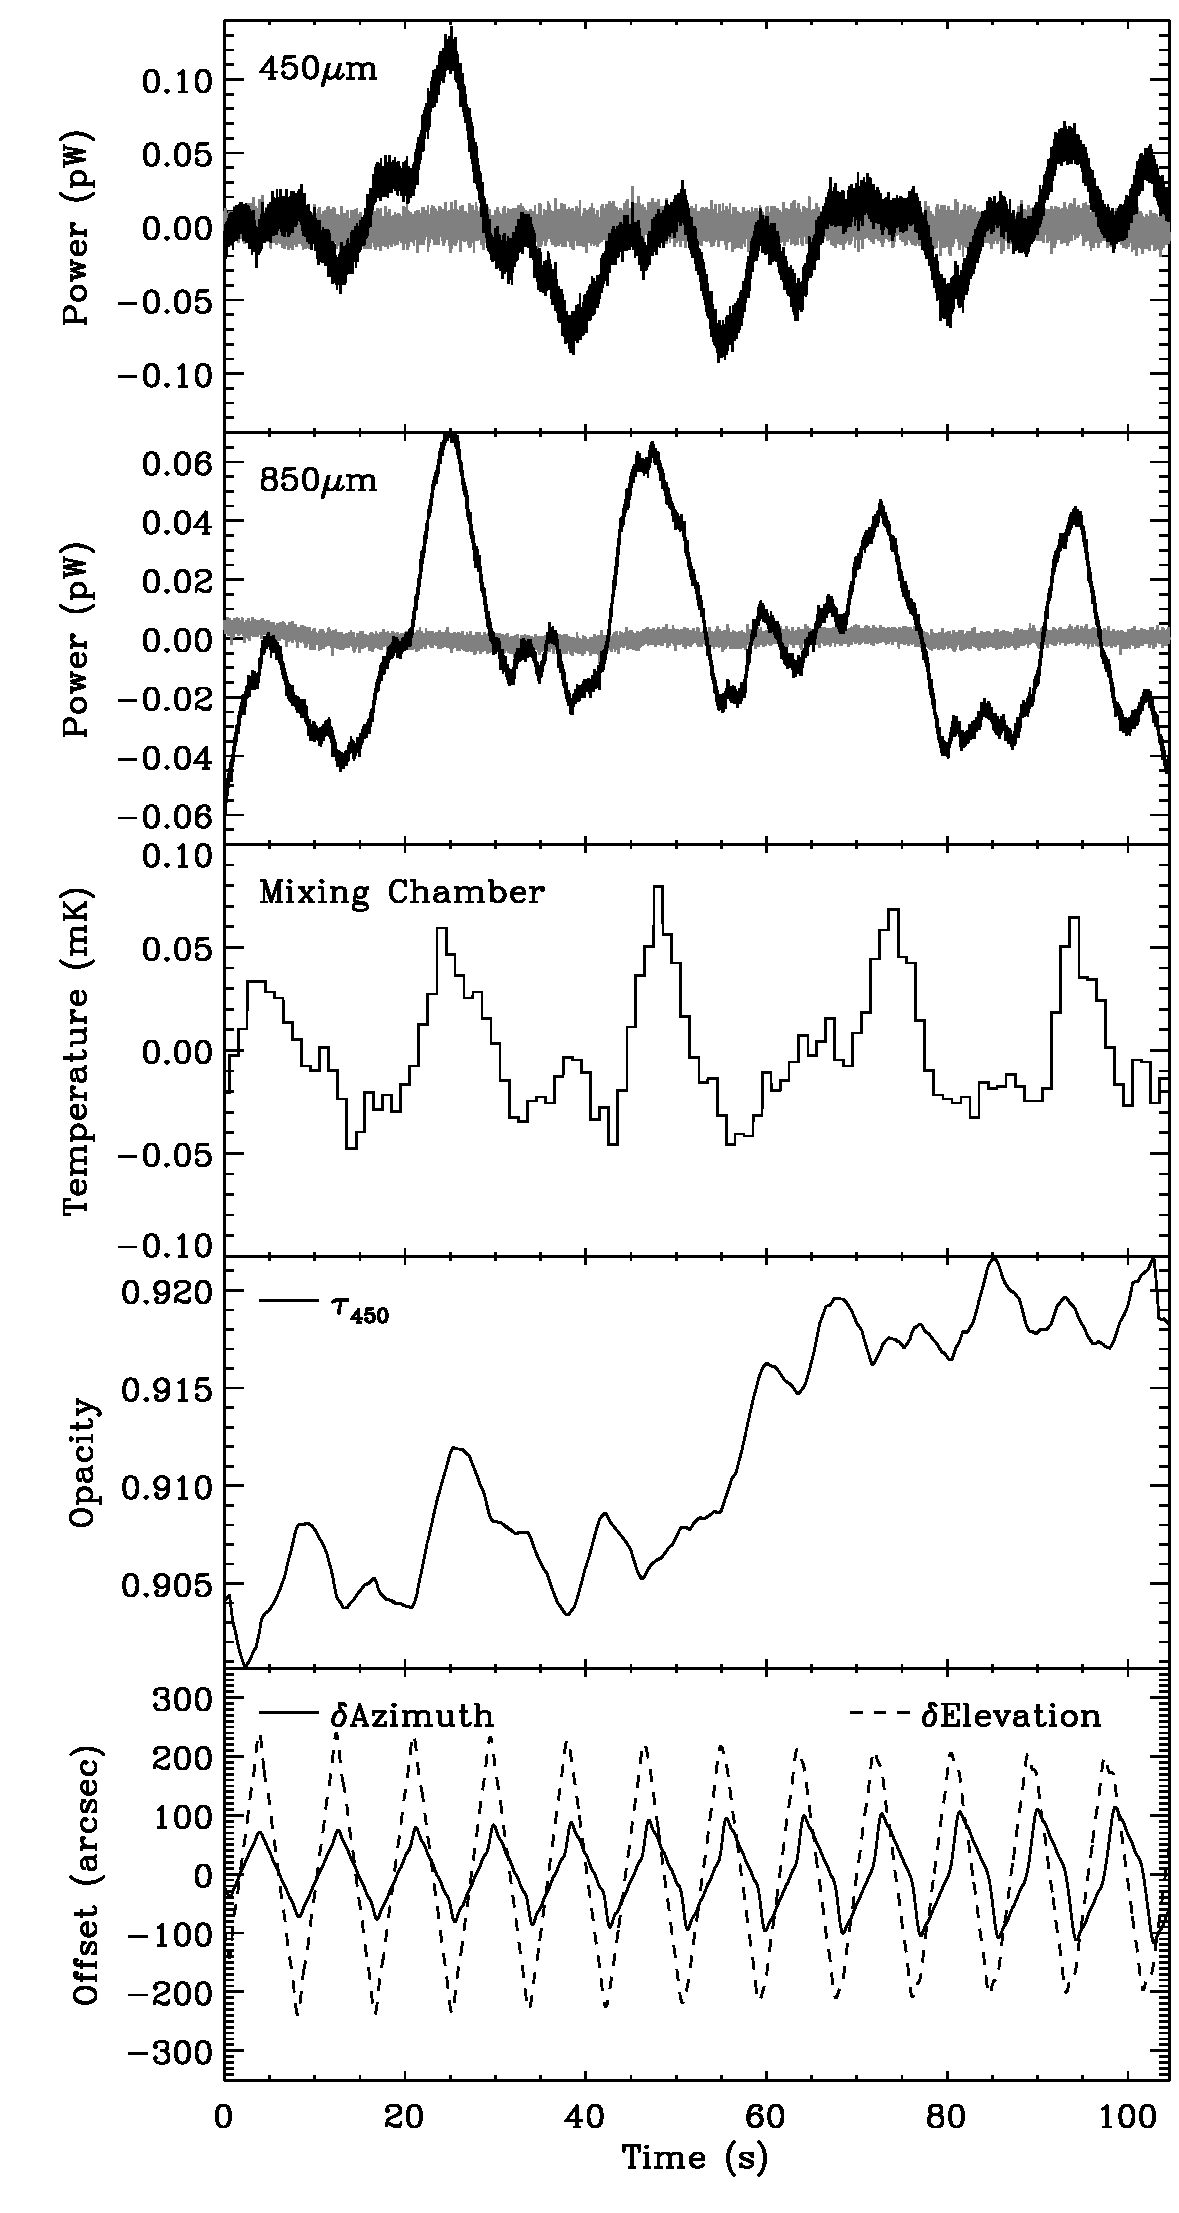
\includegraphics[width=0.49\linewidth]{bolos_point_mix_s2sro.pdf}
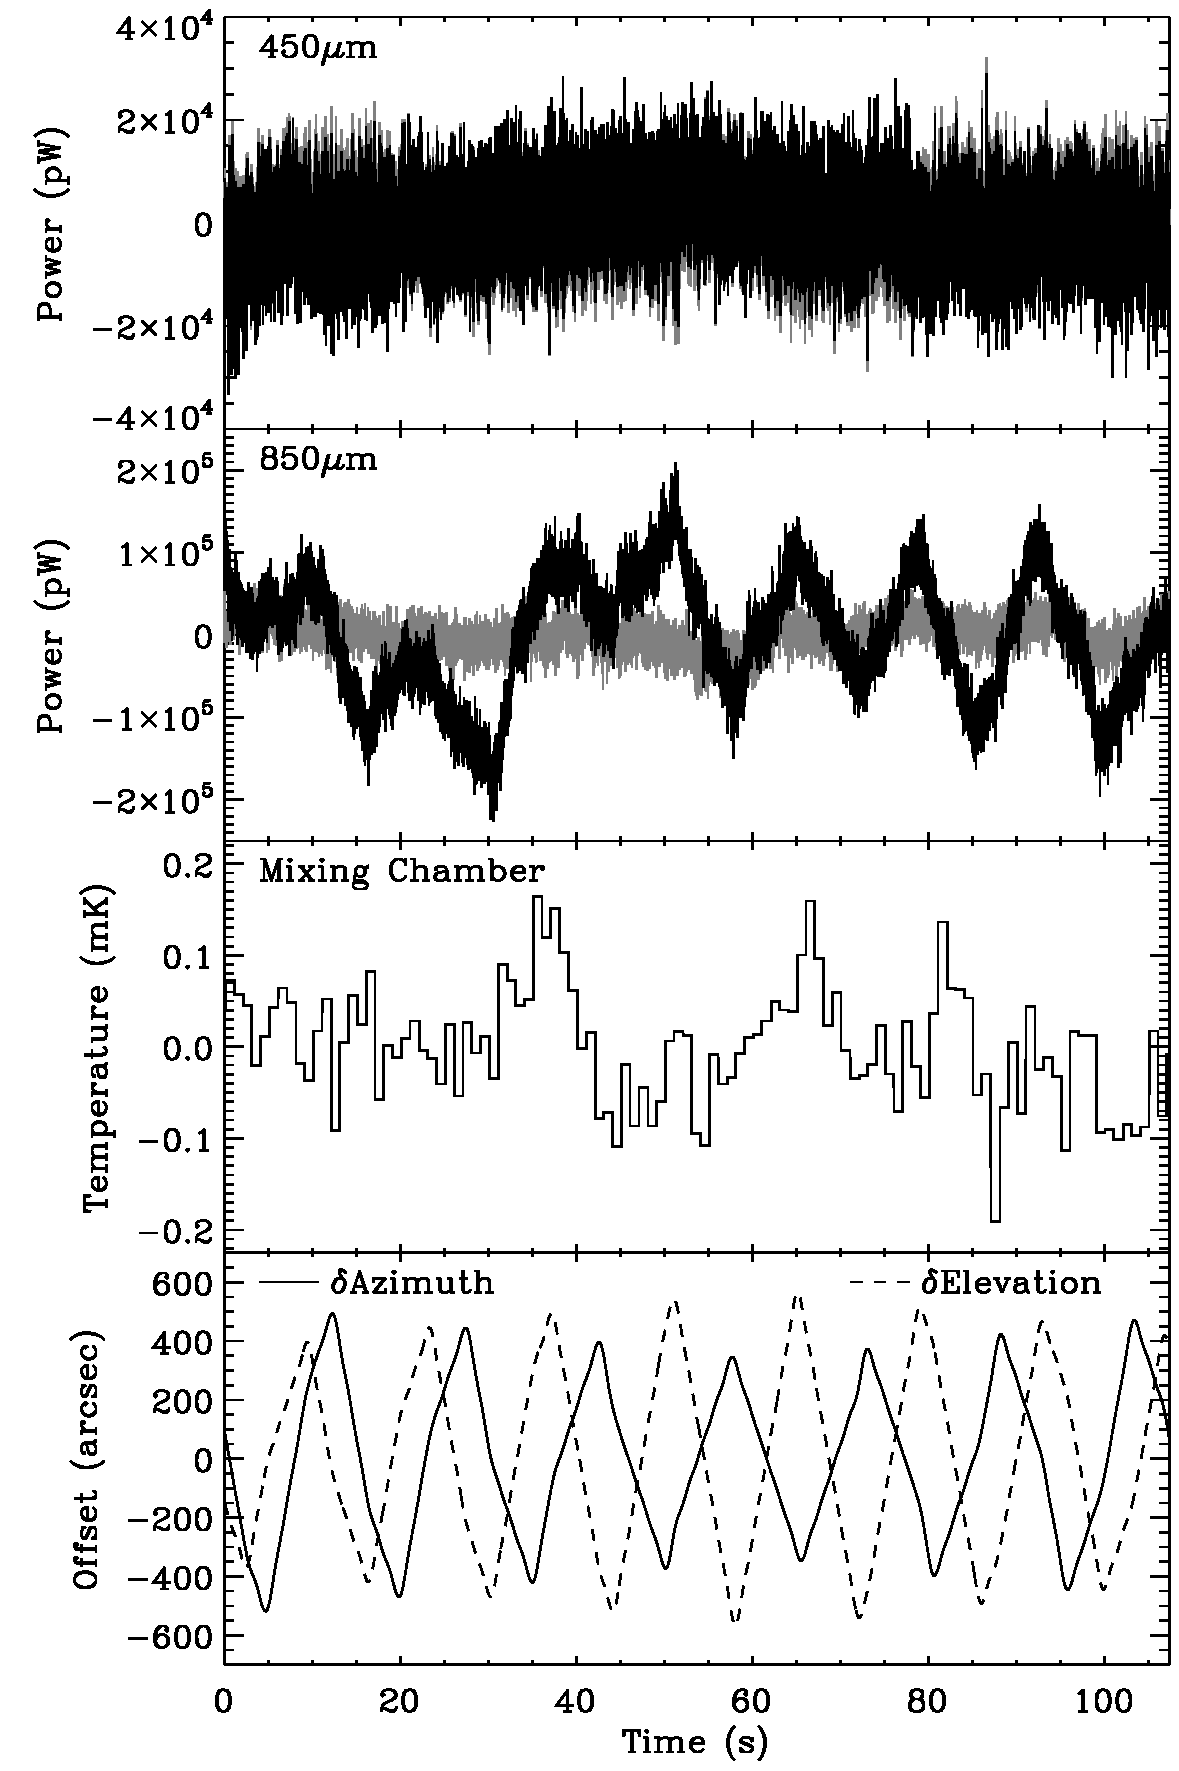
\includegraphics[width=0.49\linewidth]{bolos_point_mix.pdf}
\caption{A comparison between single bolometer time-series in each of
  the 450 and 850\,\micron\ bands with the mixing chamber temperature
  and azimuth/elevation pointing offsets, before and after upgrading
  the instrument. The grey signals over-plotted in the top two panels
  show the residual time-series after removing the common-mode
  signals.  Left: data taken during the S2SRO period, observation 29
  on 20100313. There is a strong correlation between the bolometers
  and the roughly $\sim$25\,s oscillation in the fridge, but only a
  minor correlation with the telescope motion. The nearly flat
  common-mode subtracted signals show: (i) that most of the
  low-frequency signal is common to all of the bolometers; and (ii)
  the non-correlated, and predominantly white noise at 450\,\micron\
  is significantly larger than at 850\,\micron. Right: data taken with
  the fully-commissioned instrument, observation 38 on
  20111112. Unlike the S2SRO data, there is no strong signal produced
  by variations in the fridge temperature. The 450\,\micron\ data have
  minimal correlated low-frequency noise (as evidenced by the lack of
  a difference between the raw and common-mode subtracted signals),
  although the 850\,\micron\ data show a common signal correlated with
  the telescope motion (note that this scan has a significantly larger
  amplitude than the S2SRO data set), mostly likely caused by magnetic
  field pickup (see Section~\ref{sec:magpickup} and
  Fig.~\ref{fig:magpickup}).}
\label{fig:bolos_mix}
\end{figure*}

\begin{figure*}
\centering
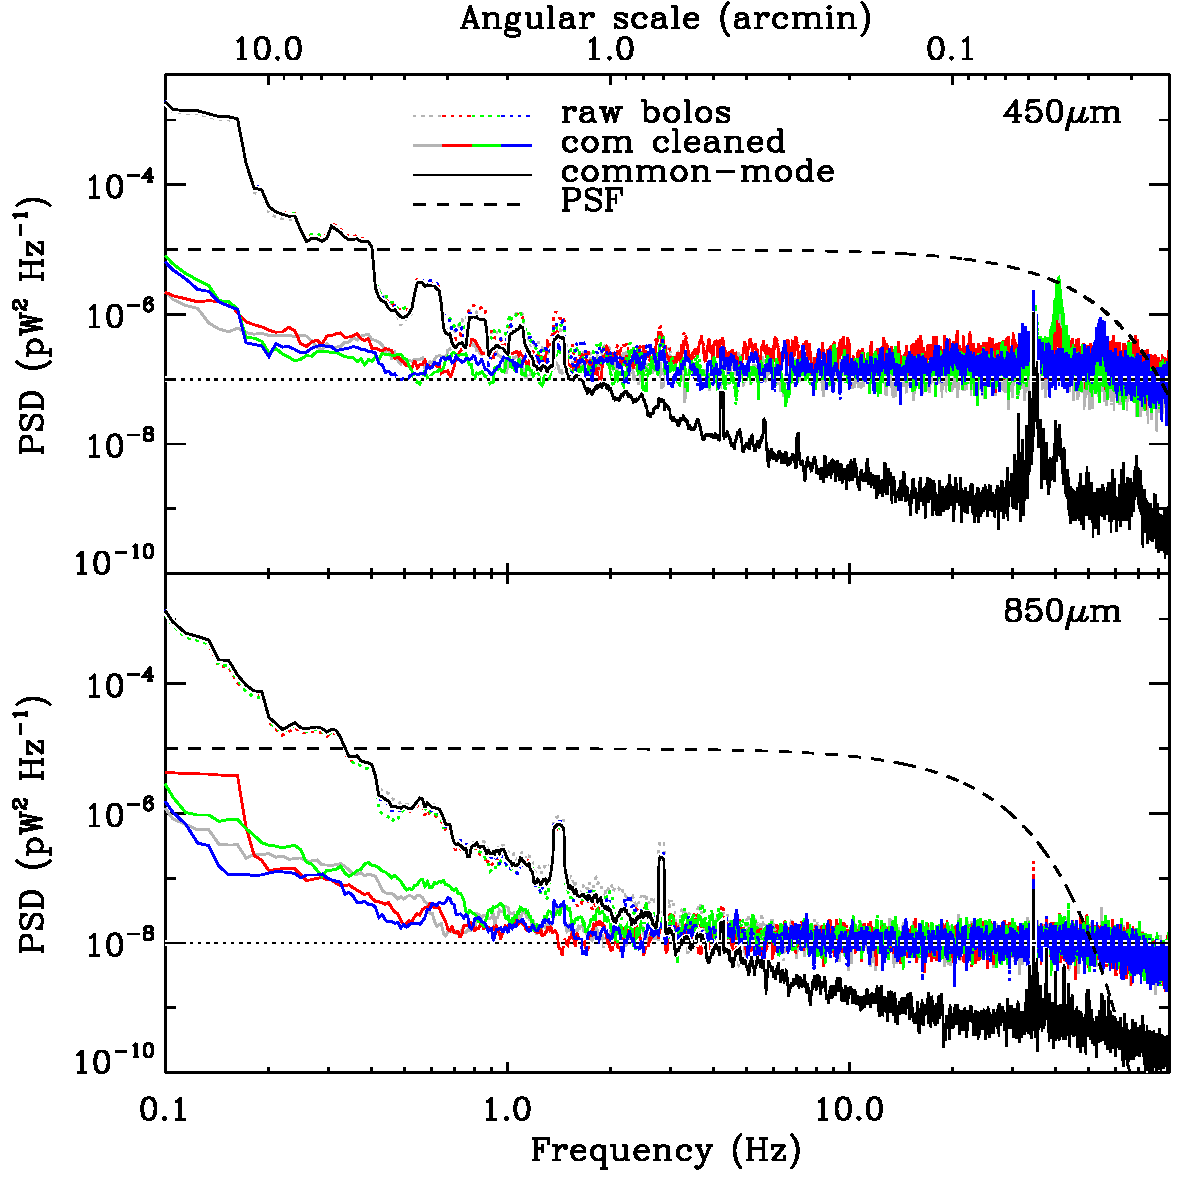
\includegraphics[width=0.49\linewidth]{pspec_s2sro.pdf}
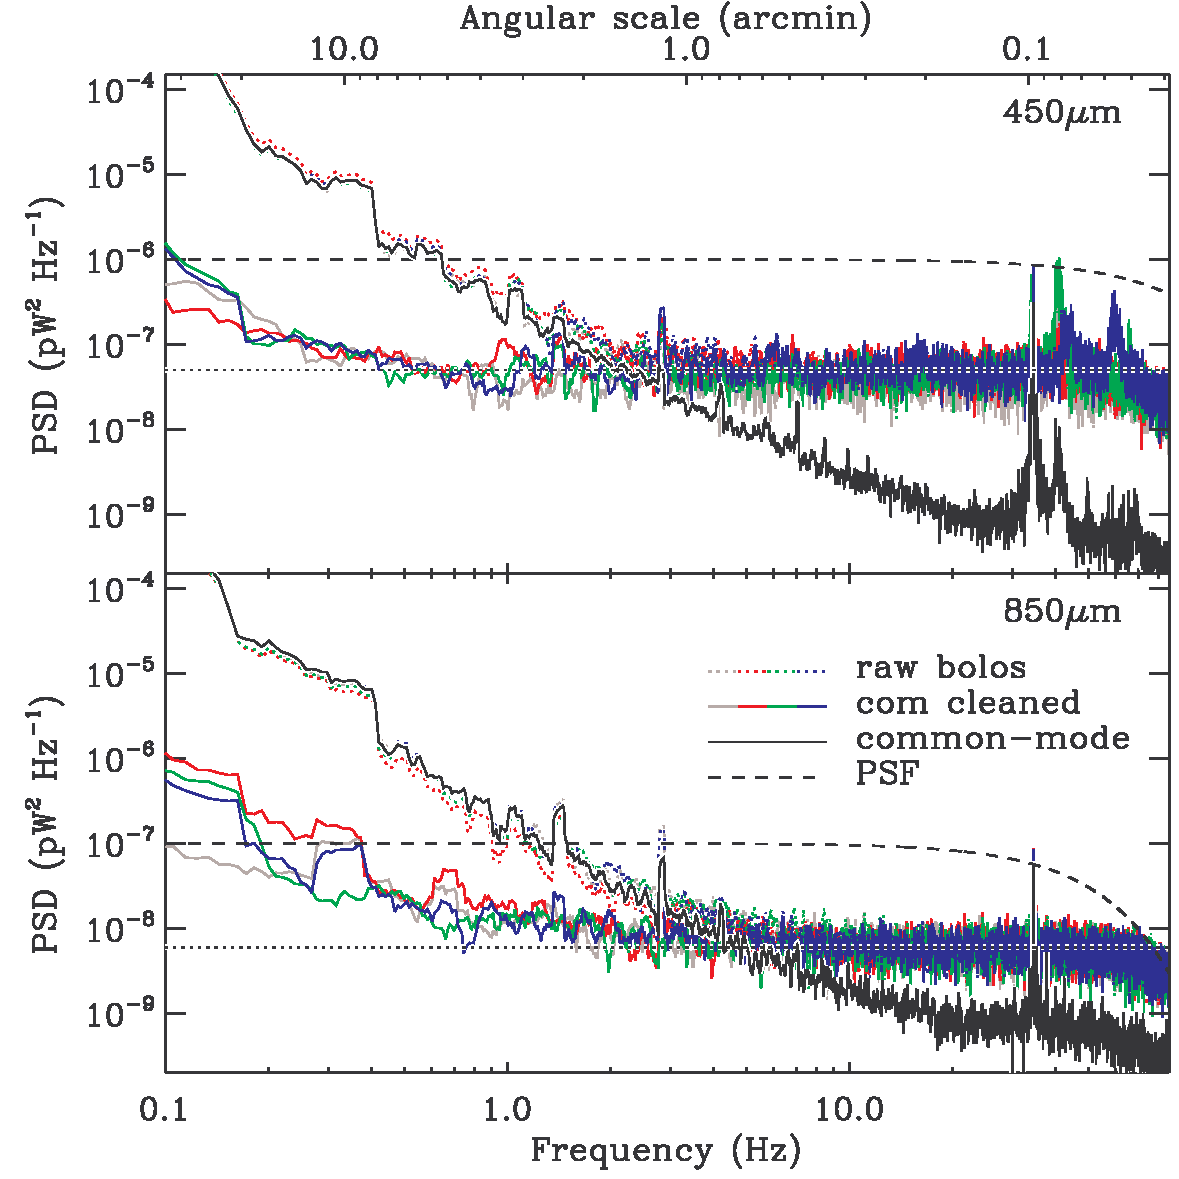
\includegraphics[width=0.49\linewidth]{pspec.pdf}
\caption{Bolometer power spectral densities for the same two data sets
  (before and after upgrades) used in Fig.~\ref{fig:bolos_mix}. The
  PSDs have been boxcar smoothed with a width of 0.1\,Hz to reduce the
  noise slightly and clarify some features. Four of the most sensitive
  bolometers have been selected at each wavelength, and the
  flat-fielded and step-corrected (but otherwise raw) PSDs are shown
  as coloured dotted lines (the blue signals are for the same time
  series as those shown in Fig.~\ref{fig:bolos_mix}).  The solid black
  lines are the PSDs of the common-mode signals at each wavelength,
  and the solid coloured lines show the PSDs of the bolometers once
  the common-mode is removed.  Finally, the dashed black lines show
  the spectral shape produced by a point source given the scan speeds
  for the two observations (120\,arcsec\,s$^{-1}$ in the left-hand
  plot, and 190\,arcsec\,s$^{-1}$ in the right-hand plot); for
  reference, the top horizontal axes shows the conversion from
  frequency to angular scale. Horizontal dotted lines at $2 \times
  10^5$ and $1 \times 10^5$\,pW\,Hz$^{-1}$ at 450 and 850\,\micron,
  respectively, are provided as a visual reference for the white-noise
  levels. In addition to $1/f$ and white noise components, and line
  features, all of the PSDs exhibit the gradual roll-off of the
  anti-aliasing filter just below the Nyquist frequency.  Left: for
  the S2SRO data there are broad line features in the PSDs at both
  wavelengths above $\sim$35\,Hz.  At lower frequencies, the bolometer
  signals exhibit clear $1/f$ knees at approximately 1 and 2\,Hz at
  450 and 850\,\micron. Common-mode subtraction removes most of the
  correlated fridge oscillation signal, lowering the $1/f$ knees to
  approximately 0.2 and 0.7\,Hz at 450 and 850\,\micron,
  respectively. Right: data from the fully-commissioned instrument
  tend to have lower $1/f$ knees, and fewer line features. The
  remaining low-frequency noise, now that the fridge oscillations have
  been removed, is considerably more independent from bolometer to
  bolometer than in the S2SRO data (note the larger spread in the
  dotted lines at low frequencies compared to the left-hand plot,
  particularly at 450\,\micron). Finally, this example shows that the
  white noise performance is in fact similar for the two subarrays
  (s4a and s8b) that were used both before and after the upgrades.}
\label{fig:pspec}
\end{figure*}


%-------------------------------------------------
\subsection{Typical bolometer signals}
\label{sec:bolosignal}
%-------------------------------------------------

In Fig.~\ref{fig:bolos_mix} we show sample time-series from single
bolometers in each of the 450 and 850\,\micron\ focal planes, as well
as variations in the mixing chamber temperature (as a proxy for the
focal-plane temperature), and the telescope pointing, for two data
sets, before and after the upgrades that followed S2SRO.

In the S2SRO data (left panel), observation 29 on 20100313, both
bolometers share significant long-timescale structure ($\gsim10$\,s)
that appears to be related to variations in the fridge base
temperature, although the similarity is clearly greater at
850\,\micron. In this particular case, the total power in the
fluctuations at 450\,\micron, are comparable to those at
850\,\micron. Such behaviour might be expected if there is a
comparable varying thermal load from the fridge at each wavelength
that dominates. We also note that there is no obvious strong
correlation between the low-frequency signal structure, at either
wavelength, with the telescope motion.

The low-frequency signal component of the S2SRO bolometer output is
also highly correlated amongst bolometers in the same subarray. We
have calculated a common-mode signal, $\mathbf{c}(t)$, as the average
time-series of all the working bolometers. We then fit the amplitude
of $\mathbf{c}(t)$ at each wavelength to the signals shown in
Fig.~\ref{fig:bolos_mix} and remove it, yielding the grey residual
signals. These residuals are quite flat, although still with
noticeable variations. The white noise is also apparent, and larger at
450\,\micron\ as one would expect from the larger backgrounds compared
to 850\,\micron.

Data from the fully commissioned instrument, observation 38 on
20111112, are shown in the right panel of
Fig.~\ref{fig:bolos_mix}. Having solved the fridge oscillation
problem, these data no longer exhibit a correlation with the mixing
chamber (note that variations are still seen in the mixing chamber;
however, such variations do not necessarily reflect changes in the
focal plane temperature). There is minimal correlated low-frequency
noise in these 450\,\micron\ data (note that there is almost no
difference once the common-mode has been subtracted). The
850\,\micron\ channel, however, exhibits a more significant signal
that is obviously correlated with the telescope motion. It is also
correlated amongst many of the detectors, and common-mode removal
corrects it to some extent. Part of the reason that this is seen here,
and not in the S2SRO data set shown, is that the amplitude of the scan
pattern is larger. Most of this ``scan-synchronous'' noise is
attributed to magnetic field pickup, as described in
Section~\ref{sec:magpickup}.

Next, in Fig.~\ref{fig:pspec} we produce power spectral density (PSD)
plots for four of the most sensitive bolometers from both focal
planes, using the same two data sets. To produce this figure, we
follow the convention that the PSD as a function of frequency,
$\mathbf{P}(f)$, is normalised such that the integral over frequency
gives the same variance as the time-series variance across the full
time-series. In other words, given a bolometer signal $\mathbf{b}(t)$,
%
\begin{equation}
\label{eq:psd}
\langle\mathbf{b}^2(t)\rangle = 2 \int_0^{f_\mathrm{N}} \mathbf{P}(f)
df ,
\end{equation}
%
where we only integrate over the positive frequencies up to
$f_\mathrm{N}$, the Nyquist frequency, and the factor of 2 accounts
for the (equal) power that appears at negative frequencies in the
discrete Fourier Transform. The units of the PSD written in this form
are pW$^2$\,Hz$^{-1}$.

The dotted coloured lines in Fig.~\ref{fig:pspec} show the PSDs for
raw, though flat-fielded and step-corrected (Section~\ref{sec:steps})
data. At each wavelength, and in both data sets, there are clear $1/f$
knees at frequencies ranging from roughly 1 to 2\,Hz, followed by a
predominantly white spectrum punctuated by line features at higher
frequencies, and finally a roll-off caused by the anti-aliasing filter
above $\gsim 70$\,Hz. As indicated in the previous section, the
correlation between the low-frequency components of the different
bolometer signals is large. The solid black lines in
Fig.~\ref{fig:pspec} indicate the PSDs of the common-modes
$\mathbf{c}(t)$ at each wavelength, which reproduce much of the
low-frequency structure, as well as some of the higher-frequency line
features. The $\mathbf{c}(t)$ otherwise drop substantially below the
individual bolometer PSDs at high-frequency, as expected if the
bolometers are dominated by uncorrelated white noise in that part of
the spectrum. The common-mode signals are fit to each bolometer time
series and removed as in Fig.~\ref{fig:bolos_mix}, and the resulting
PSDs are shown as solid coloured lines.  For reference, the top
horizontal axes have been converted to angular scale assuming the scan
speeds of each observation (120\,arcsec\,s$^{-1}$ in the left-hand
plot, and 190\,arcsec\,s$^{-1}$ in the right-hand plot). The power
spectra of unresolved point-sources are also shown as dashed lines in
each band (arbitrarily normalised), showing that the smallest features
resolvable by the telescope are only minimally affected by the excess
noise in the line features at these scan speeds (this may not be the
case at higher scan speeds).

In the S2SRO data (left-hand panel of Fig.~\ref{fig:pspec}), the
low-frequency noise is very correlated between the detectors (note the
tight scatter in the dotted coloured lines, and their resemblance to the
common-mode), due to it being dominated by the fridge
oscillations. Common-mode subtraction is very effective, reducing the
$1/f$ knees in both wavelengths by about a factor of 5.

Raw data from the fully-commissioned instrument (right-hand panel of
Fig.~\ref{fig:pspec}) generally have less significant $1/f$ noise as
compared with the S2SRO data. The residual low-frequency noise is
considerably less correlated amongst detectors (larger spread in the
dotted coloured lines, particularly noticeable in these 450\,\micron\
data), leading to a less drastic improvement upon common-mode
removal. However, since the data are less dominated by low-frequency
noise to begin with, the signals generally require less low-frequency
filtering to produce maps, and therefore retain larger-scale
structures than with the S2SRO data. Furthermore, there are generally
fewer line features in the PSDs of bolometers in the
fully-commissioned instrument. Finally, these two data sets illustrate
that the white noise performance (NEFD) is in fact similar before and
after the upgrades for these two subarrays (s4a at 450\,micron, and
s8b at 850\,\micron). The main improvements are reduction in
correlated and line noise features mentioned above, and the larger
number of working bolometers (approximately a factor of 4).


%-------------------------------------------------
\subsection{Magnetic field pickup}
\label{sec:magpickup}
%-------------------------------------------------

An additional noise source that is significant in only a small subset
of the data (and more so during the S2SRO period) is magnetic field
pickup. Since the bolometer signals are ultimately detected through
the amplification of magnetic fields, any additional changing fields
within the instrument will also be detected.

Example data from the 450\,\micron\ subarray s4a where pickup appears
to be significant (observation 16 on 20100228) are shown in
Fig.~\ref{fig:magpickup}. The time-series for two bolometers in the
same column (not flatfielded) show that there is a strong signal with
a similar shape, but opposite signs. This behaviour is seen across the
entire array. The dark squid signal for the same columns exhibits a
similar shape and amplitude. Since the dark squid has no thermal
absorber or TES attached to it, this observed signal is not likely to
be optical or thermal in nature (although there can be some cross-talk
with the bolometers). Due to the fact that the sign of the gain in
each stage of SQUID amplification is random (although the combined
gain is constrained to be negative), and since magnetic field pickup
is only seen at the input to the second stage, the pickup can appear
with random signs for bolometers along a column, giving it a distinct
signature from other common signals that always appear with the same
sign.

\begin{figure}
\centering
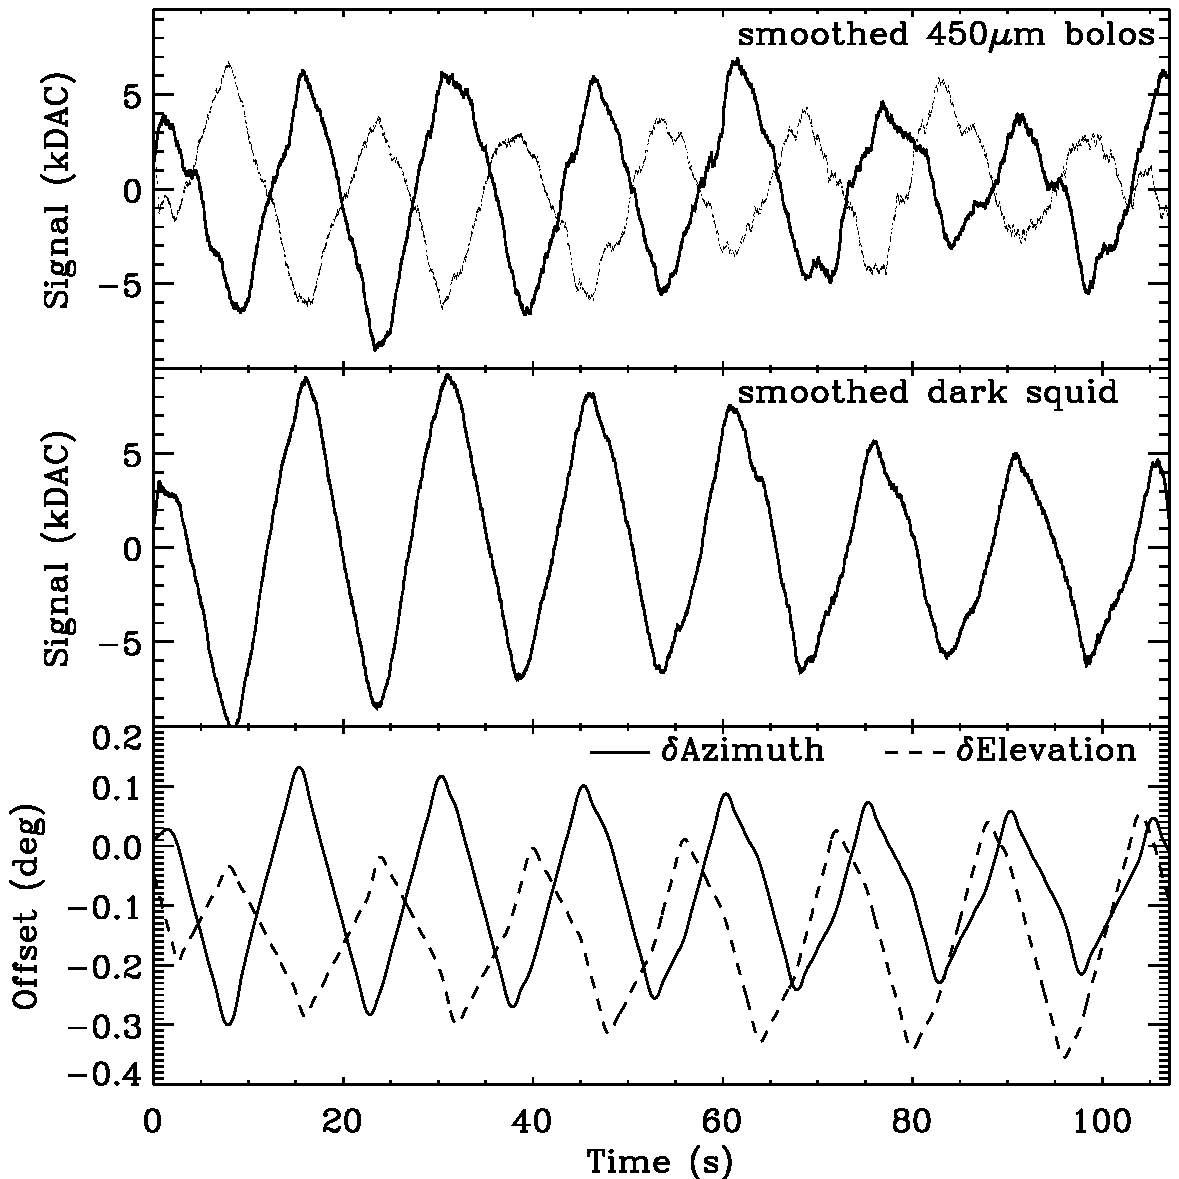
\includegraphics[width=\linewidth]{magpickup.pdf}
\caption{Evidence for significant magnetic field pickup for
  observation 16 on 20100228 at 450\,\micron\ (s4a subarray).  The top
  panel shows two un-flatfielded (but mean-subtracted and step
  corrected) bolometer time-series from the same column, with a 200
  sample boxcar smooth (approximately 1\,s), illustrating that they
  are dominated by a similar signal with opposite signs. The second
  panel shows the dark squid signal for the column, also
  mean-subtracted and with the same boxcar smooth. The bottom panel
  shows the azimuthal and elevation offsets from the map centre. For
  reference, the mean azimuth was 171.9$^\circ$ and the mean elevation
  68.0$^\circ$. Only the azimuthal signal appears to be correlated
  with the dark squids and bolometer signals, which suggests a
  magnetic field stationary with respect to the telescope dome as the
  source, since its direction with respect to the cryostat only
  changes with azimuthal motion.}
\label{fig:magpickup}
\end{figure}

The telescope pointing offsets for this approximately 0.5\,degree
diameter scan are also shown in Fig.~\ref{fig:magpickup}. Since the
phase of the azimuth offsets from the map centre in this scan pattern
slowly drifts with respect to the elevation offsets, it is clear that
the bolometer and dark squid signals are detecting a noise source that
is correlated only with the azimuthal motion and not the
elevation. This behaviour would be expected if if there were a strong
magnetic field fixed with respect to the telescope dome (i.e., the
earth's magnetic field). Since \scuba\ is mounted on a Nasmyth
platform, only azimuthal motion will change the effective direction of
such a field with respect to the cryostat. Tests have shown that, as
in this example, large scans in azimuth generically produce pickup. In
contrast, and as expected, changes in elevation results in pickup that
is approximately three orders-of-magnitude smaller.

%-------------------------------------------------
\subsection{Principal component analysis}
\label{sec:pca}
%-------------------------------------------------

\begin{figure*}
\centering
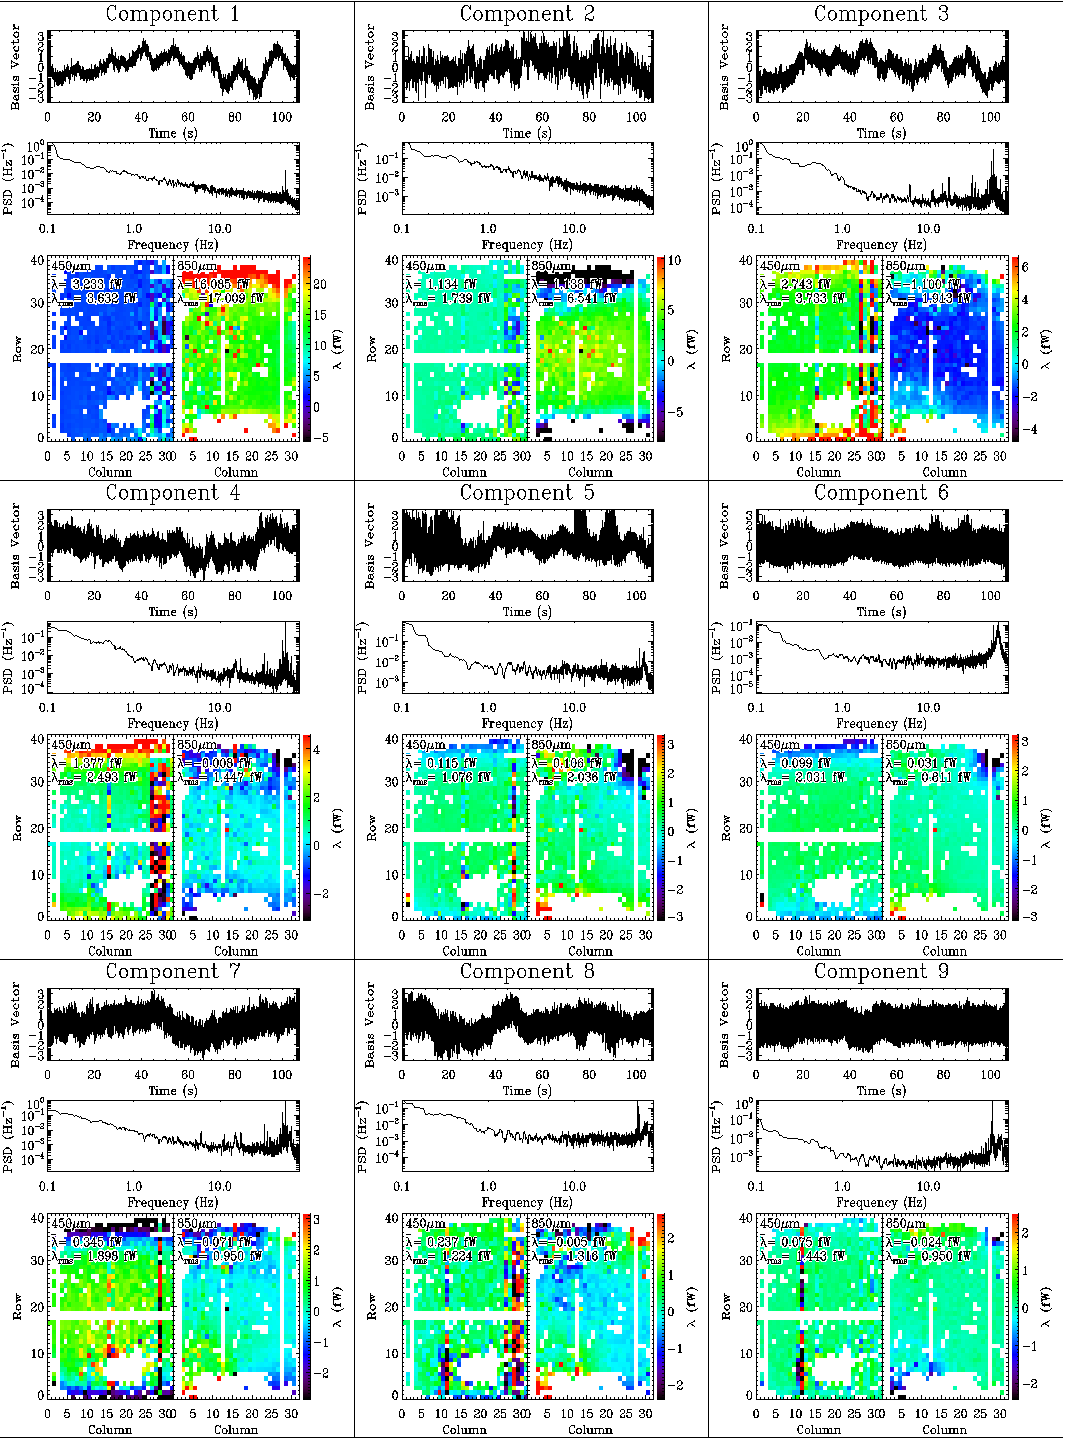
\includegraphics[width=\linewidth]{pca.pdf}
\caption{The first twelve components from a principal component
  analysis, ranked by the mean eigenvalues, of combined 450 (s4a
  subarray) and 850\,\micron\ (s8b subarray) time-series bolometer
  data, for the same observation as that used in the right-hand panels
  of Figs.~\ref{fig:bolos_mix} and \ref{fig:pspec}. For each component
  the top plot shows the time-series of the normalised eigenvectors,
  the middle plot its PSD, and the bottom coloured panels the
  eigenvalues for the bolometers at each wavelength (the amplitudes of
  the eigenvectors in the time-series). For reference, both the mean,
  $\bar{\lambda}$, and \rms, $\lambda_\mathrm{rms}$, eigenvalues for
  the bolometers in each subarray are also shown. Most of the
  correlated $1/f$ signal is encapsulated in Components~1 and 2, and
  appears to be dominated by scan-synchronous noise (compare with the
  scan pattern in the right-hand panel of Fig.~\ref{fig:bolos_mix}).
  Components~3, 4, 7 and 11 are transient glitches that only appear in
  a small subset of the bolometers. Component~5 also appears in only a
  few bolometers, and is dominated by a narrow line at 57\,Hz which
  suggests that it is related to the 60\,Hz mains. Components~6 and
  8--10 contain a mixture of broad lines above $\sim$30\,Hz (which are
  probably aliased high-frequency noise), with some low-frequency
  drifts. Finally, the erratic appearance of the eigenvector for
  Component~12 is typical of a poorly-biased detector.}
\label{fig:pca}
\end{figure*}

A method that has been used to remove correlated noise as part of the
map-making procedure for BOLOCAM and AzTEC is Principal Component
Analysis \citep[PCA,][]{laurent2005,scott2008,perera2008}. Here we use
PCA to explore correlated signals in \scuba\ data.

The basic method is as follows: (i) a covariance matrix is built up
for all pairs $(i,j)$ of the $N$ bolometer time-series,
$\langle\mathbf{b}_i(t),\mathbf{b}_j(t)\rangle$; and (ii) a singular
value decomposition identifies a new set of statistically uncorrelated
eigenvectors, $\mathbf{\xi}_i(t)$ (i.e., whose covariance matrix is
diagonal), such that each of the bolometer time-series is a linear
combination of the eigenvectors, or components i.e., $\mathbf{b}_i(t)
= \bar{\mathbf{\xi}} \mathbf{\lambda}_i^\mathrm{T}$, where each row of
the matrix $\bar{\mathbf{\xi}}$ is an eigenvector, and
$\mathbf{\lambda}_i^\mathrm{T}$ is a column vector containing the
corresponding eigenvalues. The $\mathbf{\xi}_i(t)$ are normalised by
$[\sum_t \mathbf{\xi}_i^2(t)]^{1/2}$, such that the root mean square
(\rms) amplitude of each component in a given bolometer signal is
stored in the eigenvalues. In the earlier analyses mentioned, the
low-frequency noise is assumed to be encapsulated in those components
with the largest eigenvalues. Removing the projection of the time
series along those components then significantly reduces $1/f$ noise
while retaining most of the (higher-frequency) signal in point-like
sources

A novel feature of our \scuba\ analysis is that we can perform PCA
with 450 and 850\,\micron\ data simultaneously, potentially helping us
to differentiate thermal and optical noise signals (e.g., from the
atmosphere) that might appear in both wavelengths, from other noise
sources that are restricted to single subarrays (such as readout
noise). In Fig.~\ref{fig:pca} we show the results for a combined
analysis of the s4a and s8b subarrays for the first $\sim$100\,s of
the same observation that was used in the right-hand
(fully-commissioned) panels of Figs.~\ref{fig:bolos_mix} and
\ref{fig:pspec}. The 12 most significant components are shown (ranked
by the mean eigenvalues across all working bolometers in both
bands). The top and middle panels for each component show the
time-series and PSDs of the normalised eigenvectors. The bottom panels
are maps indicating the eigenvalues (amplitudes) of the component
across the focal plane (with the mean $\bar{\lambda}$ and and \rms,
$\lambda_\mathrm{rms}$, of the eigenvalues for all of the bolometers
calculated separately at each wavelength also shown).

The majority of the correlated signal at both wavelengths in
Fig.~\ref{fig:pca} is clearly produced by Components~1 and 2. In both
cases, the eigenvector time-series exhibit a roughly periodic signal
that resembles the scan pattern in the right-hand panel of
Fig.~\ref{fig:pca}. While these correlated signals also clearly appear
at both wavelengths, referring to the maps of eigenvalues, they are
considerably stronger at 850\,\micron\ (consistent with the visual
appearance of the bolometer signals in Fig.~\ref{fig:pca}). Also note
that the PSDs for these eigenvectors exhibit nearly a pure $1/f$
signature with almost no line features, or a white-noise plateau
(suggesting that these are high-\snr\ measurements of a purely
low-frequency drift).

What is the physical interpretation of these two components? First,
the smoothly-varying pattern in the eigenvalue maps (particularly
evident at 850\,\micron) suggests that the scan-synchronous noise
(presumably magnetic field pickup) has a different response across the
focal plane; in this case the PCA may have identified two orthogonal
shapes that, when mixed in different quantities, can reproduce most of
the signal in each bolometer. It is also likely that a varying
atmospheric contribution is also included in these eigenvectors. One
would expect the atmosphere to be more significant at 450 than at
850\,\micron, although it is not obviously visible, due to the strong
presence of the scan-synchronous noise.

Next, Components~3, 4, 7 and 11 in Fig.~\ref{fig:pca} have a common
character. In all cases, the PCA appears to have identified strong,
but transient glitches that appear in only one or several bolometers,
such as the two black bolometers near column 8, row 21 at
850\,\micron\ in Component~3.

The most interesting feature of Component~5 in Fig.~\ref{fig:pca} is a
strong narrow line in the PSD at a frequency of about 57\,Hz
(suggesting the 60\,Hz mains as the culprit). The eigenvalue maps show
that it is only significant for several bolometers in the
850\,\micron\ subarray: at column 22 row 22; several bolometers at the
bottom of column 28; and more near the top-right of the subarray.

Components~6 and 8--10 in Fig.~\ref{fig:pca} have several generic
features in common. First, the PSDs exhibit moderate low-frequency
$1/f$ noise. Second, there are broad-line features at frequencies
above $\sim$30\,Hz which we believe to be aliased high-frequency
noise, in part due to the clear correlation patterns that appear along
columns in the eigenvalue maps at both wavelengths (e.g., columns 26
and 29 at 450\,\micron in Component~6). Finally, these components also
have potentially unrelated features mixed into them, like sudden
offsets that are likely residuals due to imperfect step correction
(e.g., $\sim$50\,s in the eigenvector time-series for Component~6; also
see Section~\ref{sec:steps}).

Finally, Component~12 in Fig.~\ref{fig:pca} is again significant in
only a handful of detectors in the 850\,\micron\ subarray (e.g., column
21 row 25). The time-series plot for the eigenvector exhibits a large
positive tail of sudden excursions which gradually worsen over
time. Bolometers that exhibit this signal are probably poorly biased.

This example illustrates some of the types of correlated signals and
patterns that PCA can identify in \scuba\ data. While there are
typically one or two strong signal components detected, in general,
the details can vary significantly from data set to data set, and the
lengths of the time-series analysed. The reason for this is probably
due to the fact that many of the noise sources are not stationary in
time (e.g., scan-synchronous noise which obviously depends on the scan
pattern). It should also be clear from this example that while PCA
offers some helpful insight into the various sources of noise, it does
not necessarily identify clean patterns that can easily be
modelled. For example, while there are clearly correlation patterns
along columns (Components~6 and 8--10, particularly at 450\,\micron),
as one might expect given the common amplification chain, the
intensities of these high-frequency signals are random in the
eigenvalue maps, and a common-mode signal estimated from the data for
each column would not remove it.

%------------------------------------------------------------------------------
\section{Production of maps}
\label{sec:algorithm}
%------------------------------------------------------------------------------

\begin{figure}
\centering
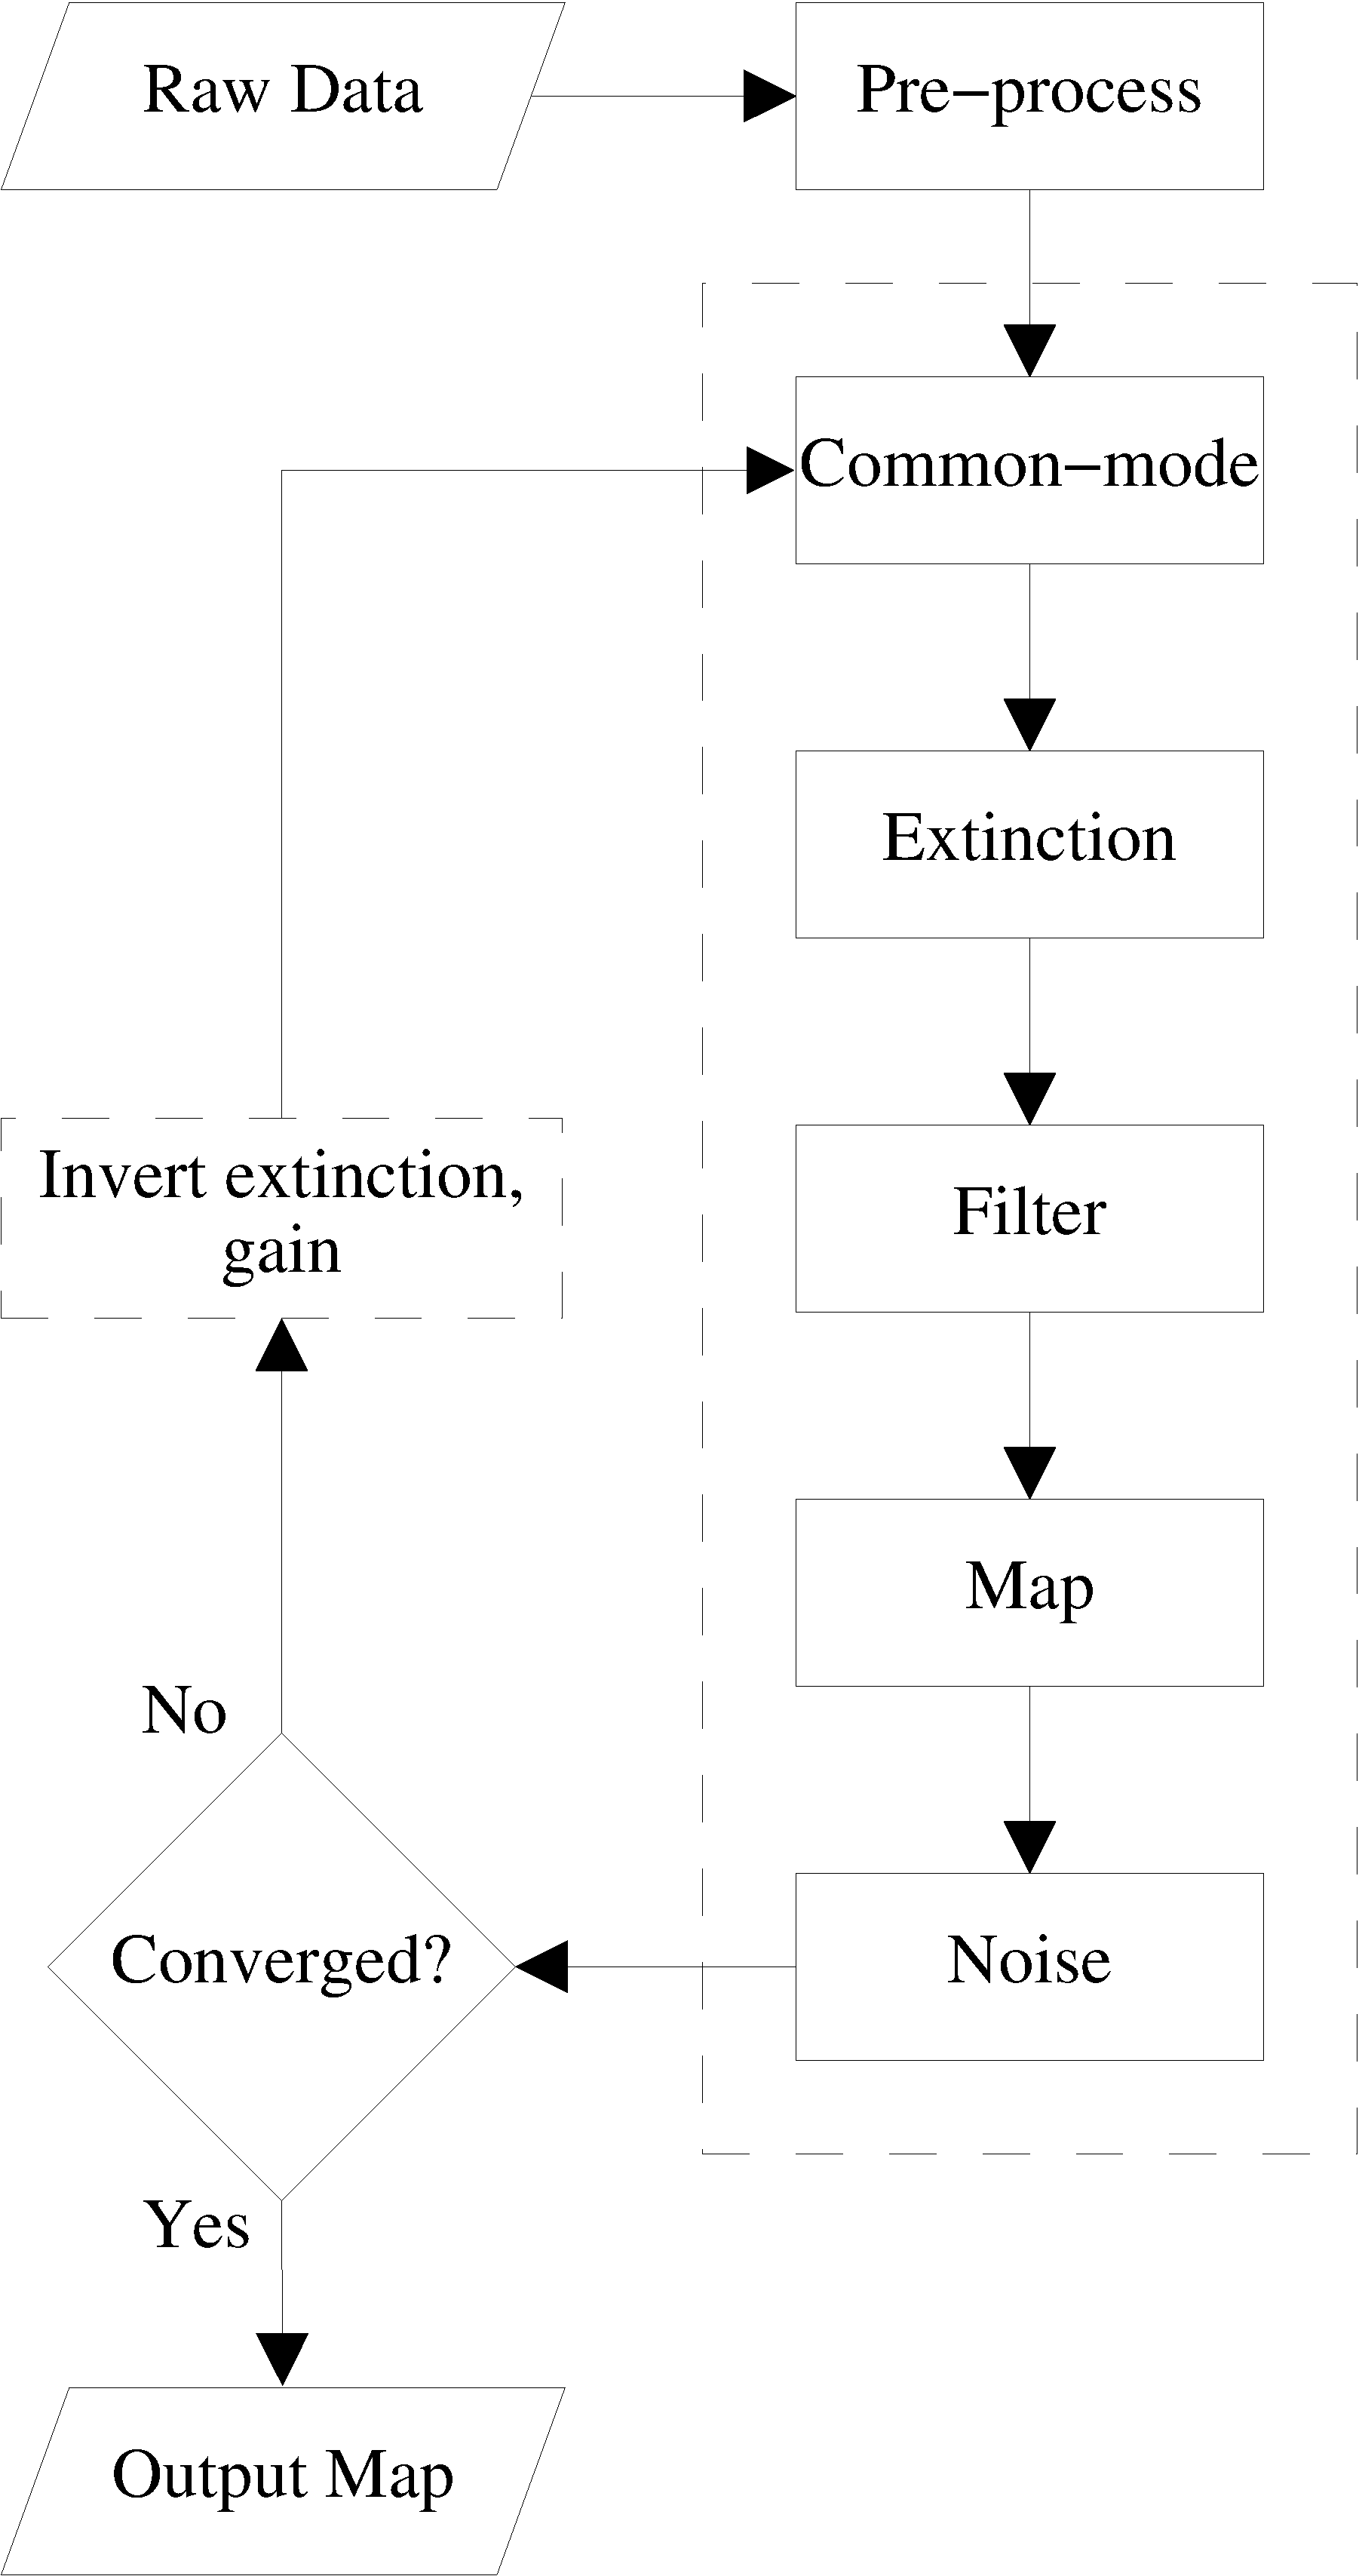
\includegraphics[width=0.75\linewidth]{dimm.pdf}
\caption{Typical map-making algorithm. Raw data (stored in multiple
  files) are read and concatenated into continuous time-series. A
  pre-processing stage repairs DC steps, applies a flatfield
  correction, and identifies and removes the noisiest bolometers. The
  iterative portion then begins: estimating and removing the
  common-mode signal; applying the extinction correction; high-pass
  filtering to remove residual independent low-frequency noise;
  estimating the map by re-gridding the data; and finally measuring
  the noise in the residual time-series. If the solution has
  converged, the map is written to disk. Otherwise any multiplicative
  factors that may have been applied to the data are inverted (e.g.,
  extinction correction), and then each additive component is
  re-estimated in turn, with the previous estimate first being added
  back into the time-series (and importantly, not the other
  components).}
\label{fig:dimm}
\end{figure}

As described in the introduction, the approach taken by SMURF to
reducing \scuba\ data is to model (and remove) predominantly
low-frequency noise sources that are correlated amongst detectors, and
to iterate this process along with estimates of the map. Significant
experimentation with different models for noise sources during \scuba\
commissioning required a highly flexible software framework, and a
configurable user interface. To achieve this goal, while minimizing
development time, it was decided to build SMURF as a Starlink package
\citep{2009ASPC..411..418J}, which provides access to a large suite of
libraries (including a commanding and messaging interface, astrometric
coordinate conversions and generation of standard WCS information,
file formats etc.). Furthermore, Starlink\footnote{\url{http://www.starlink.ac.uk}} is
open-source\footnote{\url{https://github.com/Starlink}},
and already used extensively at the Joint Astronomy Centre (host of the JCMT) for
many other systems \citep{jenness2011}, which helps with interoperability. Though
originally written in FORTRAN, many of the core Starlink libraries are
now ported to native C, or at least have a C interface. It was
therefore decided to develop SMURF in C as well (rather than C++, for
example, which would have required adding further dependencies to
Starlink), although we have taken an object-oriented approach. For
example, all of the data for a given noise model is encapsulated in a
C structure, and there is a standard interface for all functions that
handle models (member data and functions for the class,
respectively). In this way it is easy to extend SMURF with new
models. Parallelisation is incorporated in the most time-consuming
low-level routines using threads (e.g., performing Fast Fourier
Transforms, re-gridding the data), usually handling either independent
blocks of bolometers, or blocks of time, in each thread, depending on
the nature of the calculation. \textbf{... something about scalability
...}

\begin{itemize}

\item Discuss SMURF configurability

\item Some sort of proof/demonstration showing why the algorithm works

\item Discuss performance (execution time, memory, disk usage etc.)

\item Where do you get SMURF/starlink, usage of NDF

\item Talk about pipeline?

\end{itemize}

As we have seen in Sections~\ref{sec:bolosignal}--\ref{sec:pca},
\scuba\ data are dominated at low frequencies ($\lsim$2\,Hz) by highly
correlated signals. In addition to this $1/f$ noise, there is also
uncorrelated white noise, and finally residual correlated (but
non-astronomical) signals that appear at all frequencies with more
complicated relationships amongst groups of bolometers
(e.g., Fig.~\ref{fig:pca}). While the low-frequency noise can be
significantly reduced using simple common-mode removal (subtracting
the average signal from all bolometers at each time step), these
remaining correlated noise patterns are much more difficult to
model. Ultimately, a very simple approach has been taken to handling
these two contaminating sources, for which the main steps in a typical
reduction are shown in Fig.~\ref{fig:dimm}.

First, the raw data are passed through a pre-processing stage which
corrects some of the more significant glitches, applies flat-field
corrections etc. Next, the iterative process begins (dashed box). Most
of the low-frequency noise is removed using common-mode
subtraction. Next, the extinction correction is applied (it is done at
this stage rather than during pre-processing to avoid multiplying
large atmospheric signals by any small errors in the flatfield
correction). At this stage the data resemble the grey bolometer traces
in Fig.~\ref{fig:bolos_mix}, with some residual baseline drifts still
visible. These drifts are removed using a high-pass filter implemented
with Fast Fourier Transforms (FFTs). The residual signal is then
re-gridded to estimate the map. Finally, the map is used to estimate
and remove the astronomical signal contamination in the bolometer
data, leaving a relatively clean data set in which to measure the
white noise level of each bolometer. Since the common-mode and
filtering stages will have introduced ringing in the map in the
vicinity of bright sources, the entire process is iterated. Each
component in the dashed box of Fig.~\ref{fig:dimm} is re-calculated in
sequence. In this way, the second time the common-mode is calculated,
for example, most of the bright astronomical sources in the data have
already been removed in the previous iteration when the map was
estimated and subtracted, reducing the amount of ringing in the map
once it is re-estimated. Note that the extinction and gain denoted in
a second dashed box are multiplicative rather than additive models,
and so they must be inverted prior to the start of each iteration to
preserve the units (see Sections~\ref{sec:comgai} and \ref{sec:ext}).

In general, SMURF is highly configurable, including many options for
both the pre-processing stage and the iterative model components
(which models are used, what order they are calculated in, how they
are calculated).  In Sections~\ref{sec:dataprep} and
\ref{sec:components} we describe the data pre-processing steps and
iterative algorithm in detail. Section~\ref{sec:converge} explores
convergence tests and degeneracies between model components.


%-------------------------------------------------
\subsection{Data pre-processing}
\label{sec:dataprep}
%-------------------------------------------------

Prior to executing the iterative part of the algorithm, the data must
undergo several pre-processing steps. First, the data files are read
into memory and concatenated into continuous arrays (\scuba\ data are
broken up and written to disk every $\sim$30\,s during data
acquisition). As the data are loaded, they are multiplied by the
flatfield correction \citep[see Section~2.1 in][]{dempsey2012}. Next,
a series of data cleaning and filtering procedures are applied; these
include the removal of large glitches that may hinder the iterative
solution from converging, or simply tasks that do not need to be
iterated.

\subsubsection{Time-series down-sampling and map pixel size}
\label{sec:downsamp}

The highest useful frequency in the nominally 200\,Hz-sampled \scuba\
data is that which corresponds to the smallest angular scale that the
instrument is sensitive to. As mentioned earlier, the usual
rule-of-thumb for a Gaussian beam is to provide at least 3 samples for
each FWHM, or roughly 2.5\,arcsec for the 7.5\,arcsec 450\,\micron\
channel, and 5\,arcsec for the 14.5\,arcsec 850\,\micron\ channel. For
a typical scan speed of 300\,arcsec\,s$^{-1}$, the maximum useful
sample rate is therefore about 120\,Hz at 450\,\micron, and 40\,Hz at
850\,\micron. In order to save execution time and memory usage (both
of which scale linearly with data volume), it is clearly advantageous
to re-sample the data to these lower rates. In practice, the default
map pixel sizes are set to 2 and 4\,arcsec at 450 and 850\,\micron,
respectively (slightly over-sampled), and down-sampling occurs as the
data are loaded to match this spatial sampling given the slew speed.

The method used by SMURF to down-sample is to average together
multiple samples from the original time-series, $x_i$ to estimate the
lower-frequency output time-series, $y_j$. In general there will not
be an integer number of samples from $x_i$ in each of the $y_j$, so
fractional samples from $x_i$ are used at the $y_j$ time
boundaries. The algorithm is fast, since each sample in $x_i$ need
only be visited once. From a spectral point of view, this boxcar
average is equivalent to applying a sinc-function low-pass
filter. Such behaviour is desirable since it serves as an
anti-aliasing filter; most non-white features above the Nyquist
frequency in $y_j$ that could contaminate the output data are largely
removed.

As an alternative, we also investigated an algorithm in which the FFT
of $x_i$ is simply truncated to the target sample rate before
transforming back to the time domain (i.e., applying a hard-edged
low-pass filter). In practice the noise performance was
indistinguishable, and required slightly more execution time using
this method. It is therefore not currently available to users.

\subsubsection{Bolometer filtering}

Despite the ability of the map-maker to iteratively remove many noise
components, under some circumstances it may be desirable to filter the
data once during the pre-processing step. Three main filtering options
are available:

\begin{itemize}

\item The most commonly-used pre-processing filter is polynomial
subtraction. A polynomial of the requested order is fit and removed
from each bolometer time-series. At a bare minimum, the mean is
removed from all of the bolometers (order 0) in all reductions
described in this paper.

\item All of the filters available as part of the iterative Fourier
Transform Filter (Section~\ref{sec:flt}) can also be applied once
during pre-processing.

\item As an alternative to the iterative map-making procedure,
cleaning by principal component analysis (PCA) is available as an
experimental pre-processing option (Section~\ref{sec:pca}). The most
significant components in the analysis are identified, and the
projection of each bolometer time-series along their eigenvectors are
removed. A single parameter specifies the threshold on the amplitude
of the eigenvalues to be removed, as a number of standard deviations
away from the mean value. Subarrays are cleaned independently, once,
for the full length of each continuous chunk of data. Given the
computational expense of this method, and initial tests which showed
little improvement over simple high-pass filtering, this method has
not yet been explored in detail with \scuba\ data. However, since
systematic effects seem to come and go, it is possible that PCA could
be useful for particular data sets.

\end{itemize}


\subsubsection{Time-domain de-spiking}
\label{sec:timedespike}

Spikes of short duration and high amplitude are often seen in the time
series data. If not removed, they can cause ringing when filtering the
data. Two alternative approaches may be used to remove these
spikes. This section describes the detection and removal of spikes
within the time-series of each bolometer, and Section~\ref{sec:ast}
describes the iterative detection and removal of spikes as part of map
estimation. In practice, map-based de-spiking usually gives superior
results, and so time-domain de-spiking is switched off by default.

Each one-dimensional bolometer time-series is processed
independently. At each time slice, the median value of the current
bolometer is found in a box centred on the time slice, and containing
a specified number of time slices (typically 50). If the residual
between the time slice value and the median value is greater than some
specified multiple (typically 10) of the local noise level, the time
slice is flagged as a spike.

If the local noise level were estimated within the same box used to
determine the median value, a spike in the box would cause the local
noise level to be over-estimated severely. For this reason, the local
noise level is taken as the standard deviation of the values within a
neighbouring box on the ``down-stream'' side of the median box (that
is, the side that has already been checked for spikes). In other
words, the high end of the noise box is just below the low end of the
median filter box. This introduces a slight asymmetry in the noise,
but this should not matter unless the noise varies significantly on a
time scale shorter than the box size.

This simple algorithm is not very good at distinguishing between spikes
and bright point sources, and so the threshold for spike detection is
usually raised when making maps of bright point sources.

\subsubsection{Step correction}
\label{sec:steps}

\begin{figure*}
\centering
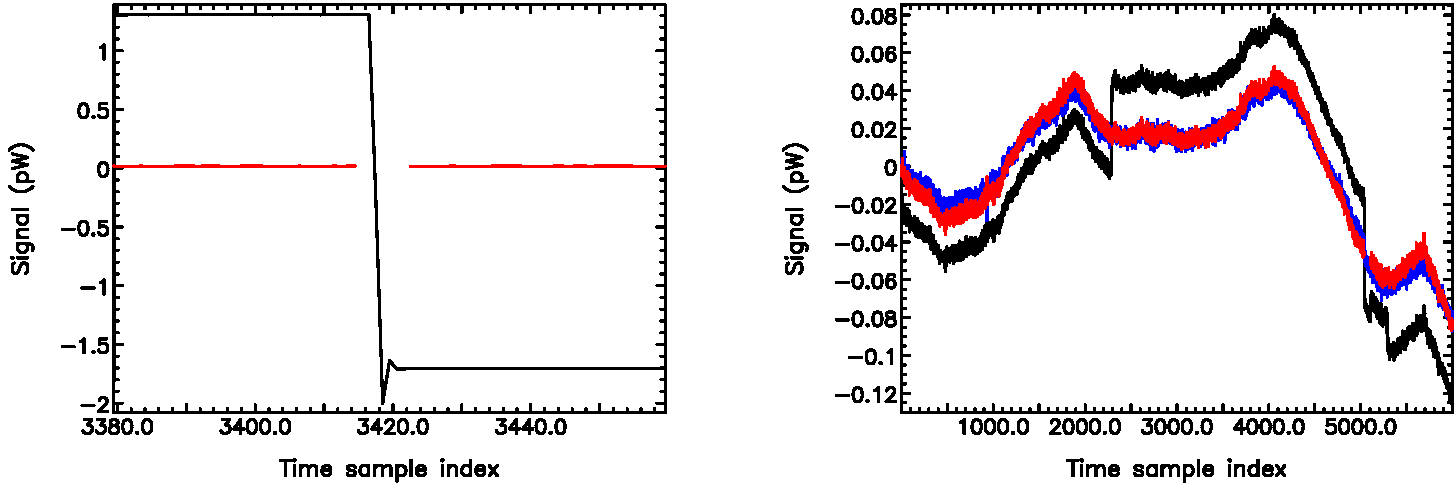
\includegraphics[width=\linewidth]{steps1.pdf}
\caption{Examples of steps in time-series data. Steps occur with a wide
range of heights from the large steps shown on the left to the small
steps shown on the right. Large steps are often followed by a brief
``over-shoot'' as shown on the left. In both plots, the black curve is
the uncorrected time-series, and the red curve is the corrected time
series. Samples close to a step are omitted in the corrected time-series.
In the right hand plot, the blue curve is the uncorrected time-series for
a nearby bolometer. The similarity between the red and blue curves shows
that the step correction is performing well.
}
\label{fig:steps1}
\end{figure*}

Sudden steps can occur in the time-series data from each bolometer,
with the most likely cause being cosmic ray events \citep[see
Section~3.5.3 in][]{holland2012}. The black curves in
Fig.~\ref{fig:steps1} show examples of such steps in the time-series
for two bolometers. If not removed, these steps can cause severe
ringing when filtering, and visible streaks in the final map,
corresponding to the paths of individual bolometers over the sky.

Steps occur with a wide range of heights and shapes. The ratio of step
height to noise can vary from less than 10 to several hundred. Some
steps occur over a single sample, such as the step close to sample
5000 in the right-hand plot of Fig.~\ref{fig:steps1}, but others
happen more gradually, such as the step close to sample 5300. In
addition, a step can be preceded or followed by a short period of
instability, as is visible at the bottom of the step in the left hand
plot of Fig.~\ref{fig:steps1} (this is probably due to the response of
the \scuba\ anti-aliasing filter; the sudden large step occurs prior
to the 200\,Hz re-sampling). Further problems are caused by steps that
occur close together in time, such as the large downward step followed
by a smaller upward step close to sample 5000 in the right hand plot
of Fig.~\ref{fig:steps1}.

Detecting and correcting such a wide variety of steps reliably has
proved to be a challenge. In outline, the following stages are
involved in detecting steps in a single bolometer time-series:

\begin{enumerate}

\item median smooth the whole time-series;

\item find the gradient of the median smoothed time-series at each
sample;

\item smooth the gradient values to determine the local mean gradient
and subtract this local mean from the total gradient to get residual
gradient;

\item find residual gradient values that exceed 25 times the local RMS
of the residual gradients;

\item Group these high residual gradients into contiguous blocks of
samples;

\item merge blocks that are separated by less than 100 samples.
\end{enumerate}

The above process produces a list of candidate steps in each bolometer
time-series. Each candidate step is then verified, measured and corrected
using the following procedure:

\begin{enumerate}

\item the above process can misinterpret the edges of a bright source
as a step, so we ignore blocks that occur close to bright sources;

\item if the block passes the above test, a least squares linear fit
is performed to the median-filtered bolometer data just before the
block, and this fit is extrapolated to predict the data value expected
at the centre of the block on the basis of the preceding data;

\item a least squares linear fit is performed to the median-filtered
bolometer data just after the block, and this fit is extrapolated to
predict the data value expected at the centre of the block on the
basis of the following data;

\item the difference between these two expected data values is taken
as the step height;

\item the preceding three steps are repeated several times, each time
including a different selection of samples in the two least squares
fits, with the mean and standard deviation of the corresponding set of
step heights found;

\item if the mean step height is small compared to the standard deviation
of the step heights, or compared to the noise in the bolometer data, then
the step is ignored;

\item if the above checks are passed, all subsequent bolometer samples
are corrected by the mean step height;

\item bolometer samples within the duration of the step, and a few
samples on either side, are flagged as unusable.

\end{enumerate}

Once all steps have been corrected within a bolometer time-series, a
constant value is added to all samples in the time-series to restore its
original mean value.

The results of step correction are shown by the red curves in
Fig.~\ref{fig:steps1}. For comparison, the blue curve shows the
uncorrected time-series from a nearby bolometer that does not suffer from
steps. The agreement between the red and blue curves confirms that
the step correction algorithm is working satisfactorily.


\subsubsection{Gap filling / apodisation}
\label{sec:gaps}

SMURF uses FFTs of the bolometer data extensively for filtering.  Data
that have been flagged as bad for any reason (for instance, due to the
presence of spikes, steps, or unusual common-mode signal) need to be
excluded from this FFT. For this reason, each contiguous block of bad
data samples is filled with artificial data before taking the FFT. A
least squares linear fit is performed to the 50 samples preceding the
block, and a similar fit is performed to the 50 samples following the
block. These are used to estimate the expected values at the start and
end of the block of bad values. The bad values are then replaced by
linear interpolation between the expected start and end
values. Gaussian noise is added with a standard deviation equal to the
mean of the RMS residuals in the two fits.

In addition to replacing bad samples before the FFT, it is also
necessary to ensure that the data values at the start and end of the
time-series are similar. Since an FFT treats the data as a single
cycle in an infinitely repeating waveform, any large difference
between starting and ending value will effectively introduce sudden
steps at the start and end of each cycle, causing unwanted
oscillations (ringing) in the transform. Another consequence of the
cyclic nature of the FFT is that features at one end of the time
series can affect the filtered values at the other end of the time
series. Two methods are available to avoid these two problems:

\begin{itemize}
\item Apodisation: a number of samples at the start and end of each
bolometer time-series are multiplied by a cosine function in order to
roll the data values off smoothly to zero. The default number of
samples modified at each end of the time-series is given by half the
ratio of the sampling frequency to the lowest retained frequency. In
addition, each end of the time-series is padded with double this
number of zeros. This method is illustrated in
Fig.~\ref{fig:pad2}. This method is not used by default as it reduces
the amount of data available for the map, and can significantly hinder
very short observations (e.g., of calibrators when focussing the
telescope).

\begin{figure}
\centering
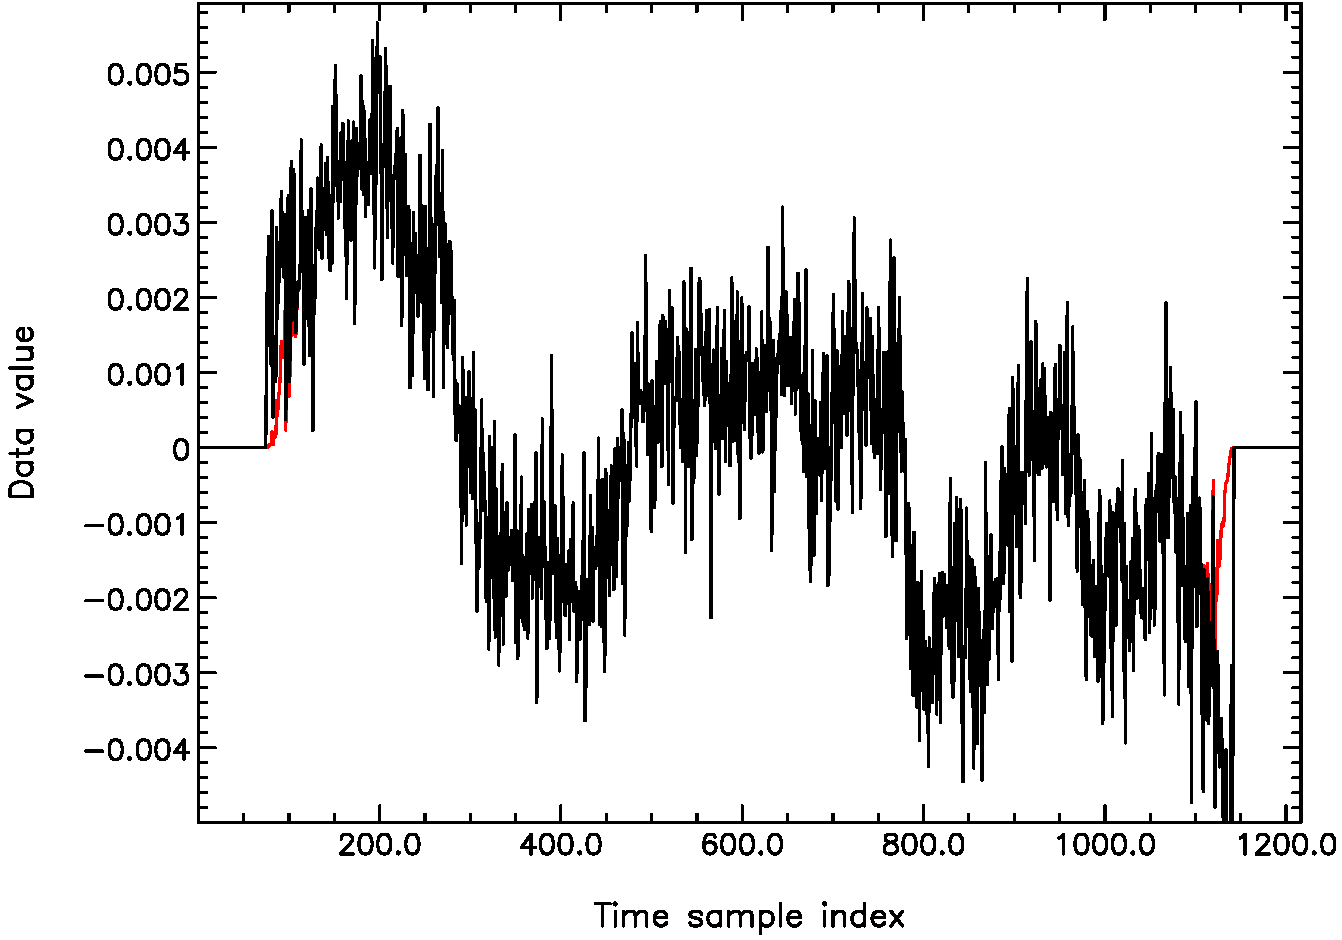
\includegraphics[width=\linewidth]{pad2.pdf}
\caption{The black curve shows a bolometer time-series, padded
with zeros. The red curve shows the time-series after apodisation.}
\label{fig:pad2}
\end{figure}

\item Padding with artificial data: instead of padding with zeros,
each time-series is padded with artificial data that connects the two
ends of the data stream smoothly and includes Gaussian noise. No
apodisation is performed. The number of samples of padding at each end
is again equal to the ratio of the sampling frequency to the lowest
retained frequency.  This is illustrated in Fig.~\ref{fig:pad1}. See
\citet{stompor2002} for a thorough discussion of this procedure within
the context of CMB map-making. This method is used by default.

\begin{figure}
\centering
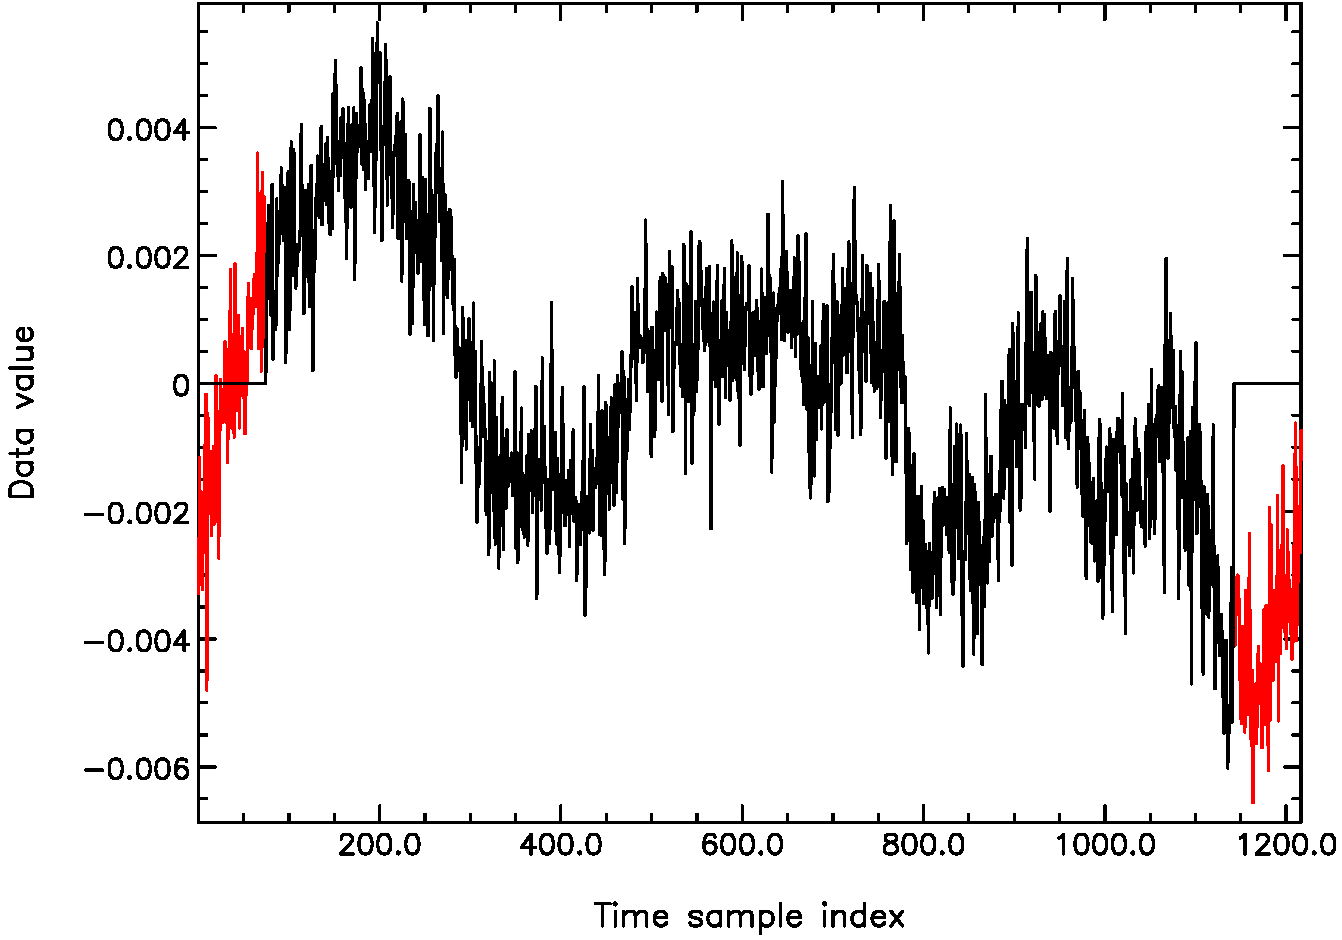
\includegraphics[width=\linewidth]{pad1.pdf}
\caption{The black curve shows the same bolometer time-series as in
Fig.~\ref{fig:pad2}, again padded with zeros. The red curve shows the
time-series after padding with artificial data.}
\label{fig:pad1}
\end{figure}

\end{itemize}

\subsubsection{Additional bad bolometer rejection}

Despite all of the cleaning operations described in the previous
sections, the data from a given bolometer may be unusable do to it
being poorly biased, having an incorrect flatfield correction applied,
or having some other particularly pathological noise
contamination. Most of these bolometers can be flagged simply by
identifying outliers in the bolometer noise distribution. By default,
SMURF measures the PSD of all bolometers between 2 and 10\,Hz, after
all other pre-processing steps have been run (identical to the
measurement in Section~\ref{sec:noi}). Despite having significant
low-frequency noise (and possibly bright astronomical source)
contamination, this higher-frequency portion of the PSD is generally
quite clean. Furthermore, even if there is contamination, the purpose
of this measurement is to identify outliers, rather than provide a
meaningful absolute measurement of a given bolometer's white noise
level. Both high and low (e.g., due to an incorrect and very small
flatfield correction being applied) outliers from the centre of the
distribution are flagged. The measurement is based on the logarithm of
the noise values, and iterative clipping of the mean and standard
deviation are used, to reduce the impact of large outliers.


%-------------------------------------------------
\subsection{Iterative model calculation}
\label{sec:components}
%-------------------------------------------------

Once the data have been cleaned, and the worst data flagged to be
ignored, the iterative solution for the map and contaminating noise
signals begins.

First, we describe the generic model for \scuba\ data. We express the
signal observed by the $i$th bolometer as a function of time,
%
\begin{equation}
\mathbf{b}_i(t) = f_i[\mathbf{e}_i(t) \mathbf{a}_i(t) + \mathbf{n}_i(t)],
\label{eq:model}
\end{equation}
%
where $\mathbf{a}(t)$ is the time-varying signal produced by scanning
the telescope across astronomical sources, $\mathbf{e}(t)$ is the
time-varying extinction, which is a function of the telescope
elevation and atmospheric conditions, and $\mathbf{n}_i(t)$ represents
sources of noise. The two terms in square brackets, as written, have
units of power delivered to the detectors (pW). The scale factor $f_i$
converts this effective power to the digitized units recorded on disk
(DAC) -- the flatfield multiplied by a digitization constant (applied
once during pre-processing) -- which in this formulation is assumed to
be constant in time.

We then express the noise, $\mathbf{n}_i(t)$, as the sum of several
components,
%
\begin{equation}
  \mathbf{n}_i(t) = \mathbf{n}^\mathrm{w}_i(t) +
  g_i\mathbf{n}^\mathrm{c}(t) + \mathbf{n}^\mathrm{f}_i(t),
\label{eq:noise}
\end{equation}
%
where $\mathbf{n}^\mathrm{w}_i(t)$ is uncorrelated white noise,
$\mathbf{n}^\mathrm{c}(t)$ is a correlated or common-mode signal (with
an optional scale factor $g_i$ for each bolometer), and
$\mathbf{n}^\mathrm{f}_i(t)$ is (predominantly low-frequency) noise in
excess of the white noise level that is either uncorrelated from
bolometer-to-bolometer, or at least does not have a simple correlation
relationship that would lead to it being included in
$\mathbf{n}^\mathrm{c}(t)$. The primary goal of map-making is to model
and remove $\mathbf{n}^\mathrm{c}(t)$ and $\mathbf{n}^\mathrm{f}_i(t)$
from the time-series, and producing a map from what is left.  This
procedure is summarized in Fig.~\ref{fig:dimm}.

Each model component is estimated from the data in a user-defined
sequence, where the typically strongest components are estimated
first, and then subtracted, leaving a cleaner signal for subsequent
model estimates. One exception to this rule is the extinction
correction, $\mathbf{e}_i(t)$ in Eq.~\ref{eq:model}, which is simply a
multiplicative factor that is known prior to map-making. Note that the
order in which this correction occurs will modify the units of
subsequently calculated additive model components (e.g., additional
brackets may be needed in Eq.~\ref{eq:model} after
$\mathbf{e}_i(t)$). Another exception is the calculation of
$\mathbf{n}^\mathrm{c}(t)$ and $\mathbf{n}^\mathrm{f}_i(t)$ in which
the previous iterations are usually added back into the time-series
simultaneously to avoid degeneracies (see Section~\ref{sec:converge}).

Usually the last two components estimated are $\mathbf{a}_i(t)$ and
$\mathbf{w}_i(t)$ once the other contaminating noise sources, and
extinction, have been corrected for. Provided that these two signals
are the only components of the residual bolometer signal, re-gridding
into a map provides the highest \snr\ estimate of the astronomical
sky. The signal produced by this map is then projected back into the
time-domain to estimate and remove $\mathbf{a}_i(t)$, leaving a
residual signal that should be dominated by white noise,
$\mathbf{n}_i^\mathrm{w}(t)$.

After the first iteration, there will almost certainly be correlated
errors between the model estimates. For example, the presence of a
bright astronomical source will contaminate $\mathbf{n}^\mathrm{c}(t)$
(which is a simple average of all of the bolometer time-series at each
instant in time), leading to an over-subtraction, and in turn,
negative bowls in the map.

Subsequent iterations, however, diminish such problems. Each additive
model component is re-estimated in the same sequence, after first
adding the previous estimate back into the time-series (but
importantly, not the other components). In this case, much of the
astronomical signal will have been identified and removed in the
previous calculation of $\mathbf{a}_i(t)$, and therefore there will be
less contamination in $\mathbf{n}^\mathrm{c}(t)$, and less negative
bowling in the map. Any multiplicative models (e.g.,
$\mathbf{e}_i(t)$) are inverted immediately prior to the start of a
new iteration to preserve the units of the data. The iterative
solution will thus converge, barring degeneracies between model
components.

The full set of model components available, and the parameters that
control them, are described in the following
sections. Table~\ref{tab:components} shows the typical order in which
they are calculated. For a discussion on convergence tests and
degeneracies, see Section~\ref{sec:converge}.

\begin{table}
  \caption{Summary of the model components that can be fit to
    \scuba\ time-series data with SMURF. Only the first group of
    models (in the order indicated) are typically fit to the data
    (\model{COM}--\model{NOI}) in the indicated order. The remaining
    models (\model{DKS}--\model{PLN}) have only been included for
    completeness}
  \vspace{0.2cm}
  \centering
  \begin{tabular}{c|l}
    \hline
    Model & Description \\
    \hline
    \model{COM} & remove common-mode signal \\
    \model{GAI} & common-mode scaled to each bolometer \\
    \model{EXT} & extinction correction \\
    \model{FLT} & Fourier transform filter \\
    \model{AST} & map estimate of astronomical signal \\
    \model{NOI} & noise estimation \\
    \hline
    \model{DKS} & dark squid cleaning along columns \\
    \model{PLN} & 2-dimensional time-varying plane removal \\
    \model{SMO} & time-domain smoothing filter \\
    \model{TMP} & pointing as baseline template \\
    \hline
    \end{tabular}
  \label{tab:components}
\end{table}

\subsubsection{\model{COM,GAI}: common-mode estimation}
\label{sec:comgai}

Fig.~\ref{fig:com} shows the time-series from a selection of typical
bolometers.\footnote{The data have been flat-fielded and each time
series has been adjusted to a mean value of zero.} The similarity
between most bolometers is evident, and forms the common-mode signal
-- assumed to be a consequence of variations in the atmospheric
emission and fridge temperature. This common-mode usually dominates
the astronomical signal for all but the brightest sources, and swamps
faint extended structure.  The purpose of the \model{COM} and
\model{GAI} models is to remove this common-mode signal.

\begin{figure}
\centering
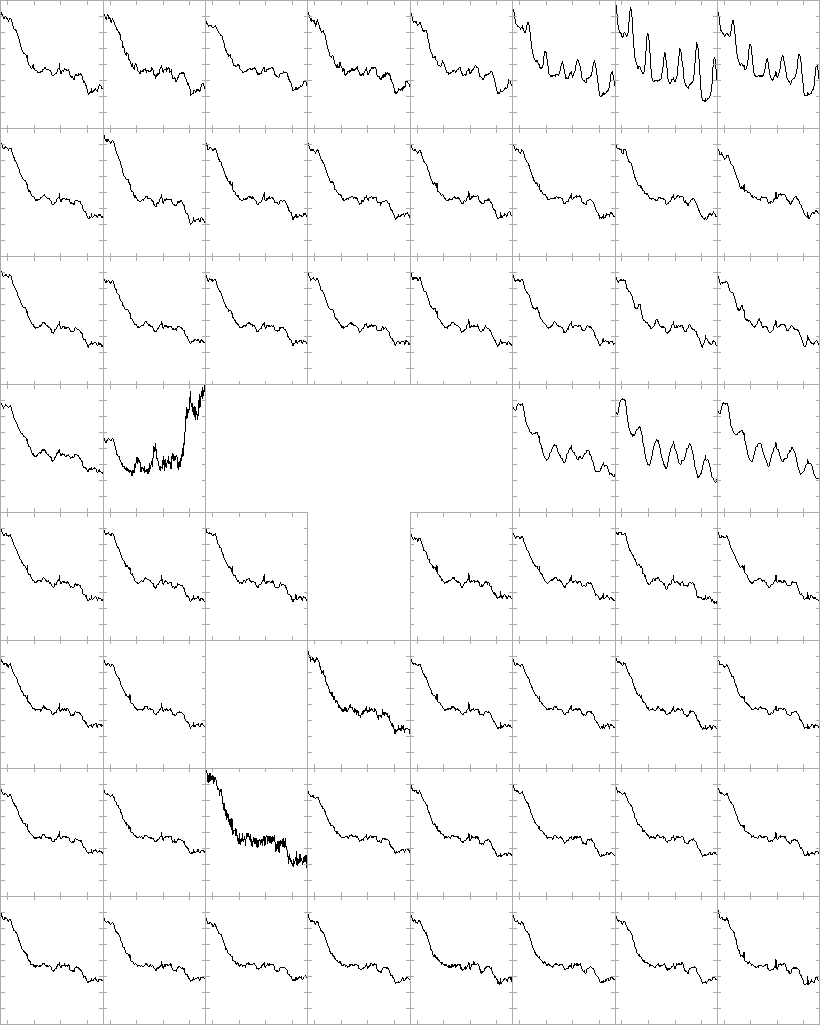
\includegraphics[width=\linewidth]{com.pdf}
\caption{A selection of typical bolometer time-series after
flatfielding and removal of a constant baseline. It can be seen that
most bolometers exhibit a common time variation overlayed with other
features. Empty squares indicate the locations of dead bolometers.}
\label{fig:com}
\end{figure}

The \model{COM} model is the common-mode signal itself
($\mathbf{n}^{c}(t)$ in Eq.~\ref{eq:noise}). It is a single time
series that is estimated by finding the mean of all bolometers at each
time step. Bolometer values that have been flagged as unusable are
excluded from the mean.

Even after flat-fielding, bolometers may have slightly varying
sensitivities and so the amplitude of the common-mode variations will
also vary from bolometer to bolometer. Comparing each bolometer time
stream with the common-mode signal allows an estimate of the relative
bolometer sensitivity to be obtained. In practice, a least squares
linear fit is performed between the bolometer time-series and the
common-mode to determine a gain ($g_i$ in Eq.~\ref{eq:noise}) and
offset for each bolometer.  The gain and offset for each bolometer is
known as the \model{GAI} model. Each bolometer value can then
optionally be scaled and shifted using these values so that all
bolometers share a common (but as yet unknown) calibration. This
provides an alternative (or additional) flat-fielding strategy to that
described in section~\ref{sec:bolos}.

An option exists to cater for time-varying sensitivities. In
principle, the gain of the bolometers should be constant in
time. However, there is evidence that there are slight variations, and
this option does tend to slightly improve the noise in maps.  If used,
the least squares fits described above are performed on short blocks
of contiguous time slices, providing multiple gain and offset values
for each bolometer (one pair for each block of time slices). The gain
and offset at any required time slice can then be found by
interpolation between these values.

It can be seen from Fig.~\ref{fig:com} that some bolometers depart
radically from the common-mode, indicating some problem within the
bolometer. Such bolometers are identified by calculating the Pearson
coefficient of correlation between each bolometer time-stream and the
common mode. Bolometers for which the correlation coefficient is below
a specified limit, or which have unusually high or low gain compared
to the other bolometers, are flagged as bad in order to omit them from
the final map. If the option described above for handling time-varying
sensitivities is used, then a correlation coefficient can be
determined for each individual block of time slices.  This allows
individual bad blocks to be rejected from a bolometer time-series,
rather than rejecting the whole bolometer. This is beneficial for
bolometers that follow the common-mode for most of the time but suffer
from transient problems at specific times. As a warning, rejecting
data based on outlier gain values can be misleading in cases where the
data are dominated by magnetic field pickup. For example, the
common-mode signal for the data in Fig.~\ref{fig:magpickup} would
resemble the azimuthal scan pattern, but clearly the gains will have
opposite signs (such that one or the other bolometer would be
erroneously flagged).

The common-mode value at each time slice is calculated as the
unweighted mean of the values of all bolometers that have not
previously been flagged as bad for some other reason. Bolometer values
that were flagged as bad simply because they were poorly correlated
with the common-mode on the previous iteration are included in the new
common-mode estimate. If such samples are excluded, there is a strong
possibility of discontinuities appearing in the \model{COM} model at
block boundaries.  These in turn can lead to ringing when filtering,
and instabilities in the convergence process.

Any astronomical sources that are smaller than the array size will
contribute signal to some bolometers but not other bolometers, thus
biassing the simple mean used to estimate the common mode. However, on
each iteration of the map-making algorithm illustrated in
Fig.~\ref{fig:dimm}, a large fraction of the remaining astronomical
signal is extracted from the bolometer time-series and transferred to the
output map, resulting in subsequent estimates of the common-mode being
more accurate.

Any extended astronomical emission on a scale comparable to or larger
than the spatial extent of the area used to estimate the common-mode
will contribute a similar signal to all bolometers. Therefore such
extended emission is indistinguishable from the other sources of
common-mode signal (e.g., atmosphere variations) and will be removed by
the model. This places a limit on the spatial extent of astronomical
structure that can be recovered.

For this reason, the usual practice is to estimate a single
\model{COM} model by examining data from all four sub-arrays in each
waveband, since this allows spatial structure on the scale of the
whole focal plane to be recovered. However, sometimes there is
evidence that the common-mode differs from one array to another, and
so an option exists to estimate a separate \model{COM} model for each
individual subarray, with a consequent lowering in the scale of
spatial structure that can be recovered.

\subsubsection{\model{EXT}: extinction correction}
\label{sec:ext}

The extinction correction is a multiplicative factor that is normally
derived using the JCMT water vapour monitor (WVM), and is not
considered to be a free parameter in the solution ($\mathbf{e}_i(t)$
in Eq.~\ref{eq:model}). However, it is applied as part of the
iterative solution, rather than a pre-processing step, since any small
errors will be amplified by the large low-frequency drifts in the raw
bolometer time-series. For example, if the bolometer drift is 1000
times greater than an astronomical source of interest, a 1 per cent
error in the flatfield will produce stripes of order 10 times the
astronomical signal amplitude in the final map! If \model{EXT} is
applied after the bulk of the low-frequency noise has been removed
(e.g., \model{COM,GAI}), then there is little potential for such small
errors to affect the final map.  For details on how it is calculated
see \citet{dempsey2012}. Note that its numerical value is calculated
only once, and simply applied as a scale factor in the iterative
solution. Unlike the additive model components, it is inverted at the
start of each iteration to preserve the amplitude of the data before
the re-calculation of other model components.

\subsubsection{\model{FLT}: Fourier transform filter}
\label{sec:flt}

This model takes the FFT of the bolometer time-stream data, and can
apply both high- and low-pass filters, as well as notch filteres, at
hard frequency edges specified by the user. Alternatively, the
frequency edges of the filters may be defined in terms of an angular
scale, but converted into a frequency through knowledge of the mean
telescope slew speed. The time-series may optionally have apodisation
applied before the transform to avoid ringing (primarily caused by
wrap-around discontinuities at the ends of the time-series). Finally,
a whitening filter may also be applied in which a simple $1/f^\alpha +
\mathrm{constant}$ is fit to the power spectrum of each bolometer, and
then the bolometer FFT is multiplied by its inverse (though normalised
to preserve the white noise level).  The signals that are removed from
the time-series by this process are stored in the \model{FLT}
container array. Typically this model is used purely as a high-pass
filter to remove most of the residual uncorrelated $1/f$ noise
following common-mode removal ($\mathbf{n}^\mathrm{f}_i(t)$ in
Eq.~\ref{eq:noise}). Low-pass filtering is redundant for two reasons:
(i) SMURF already low-pass filters and re-samples to a lower sample
rate, as described in Section~\ref{sec:downsamp}; and (ii) the act of
re-gridding the data to produce map estimates effectively low-pass
filters the data at a frequency that corresponds to the inverse of the
crossing time of a single map pixel. Notch filters have not been
proven to be useful with \scuba\ data, particularly since line
features tend to move around (i.e., a dynamic line-detection system
would have to be developed, and care would have to be taken that
astronomical sources are not suppressed).

\subsubsection{\model{AST}: map estimation}
\label{sec:ast}

Map estimation is accomplished using a nearest-neighbour resampling of
the data onto a pre-defined map grid with. For the $i$th map pixel
$\mathbf{m}(x_i,y_i)$, the brightness is estimated as the weighted
average of the bolometer data samples $\mathbf{b}_j$ that land within
that pixel (from any bolometer or point in time),
%
\begin{equation}
  \mathbf{m}(x_i,y_i) = \frac{\sum_j \mathbf{w}_j \mathbf{b}_j }
                             { \sum_j \mathbf{w}_j } .
\end{equation}
%
For the initial iteration the weights $\mathbf{w}_j$ are set to 1, but
subsequently they are set to $1/\sigma_j^2$, the estimated inverse
variance expected from the bolometer white noise levels, as discussed
in Section~\ref{sec:noi}. This weighting scheme is sensible provided
that the bolometer data have no correlated (i.e., low-frequency)
noise.

In addition to the signal map, a variance map $\mathbf{v}(x_j,y_j)$ is
estimated. The default behaviour is to estimate this weighted error on
the mean given the scatter in the weighted samples. This is
accomplished by dividing the biased weighted sample variance by the
number of samples that went into the average (akin to the formula for
standard error on the mean, but accounting for weights),
%
\begin{equation}
\label{eq:varmap}
\mathbf{v}(x_j,y_j) = \frac{\sum_j \mathbf{w}_j
                            \sum_j \mathbf{w}_j \mathbf{b}_j -
                            \left( \sum_j \mathbf{w}_j \mathbf{b}_j \right)^2 }
                           { N \left( \sum_j \mathbf{w}_j \right)^2 },
\end{equation}
%
where $N_j$ is the total number of bolometer samples that land in the
pixel. As written, this algorithm is numerically unstable if the two
terms in the numerator are large, and of nearly the same value:
floating point precision errors can cause the difference to be
significantly incorrect. In practice we use the more numerically
stable ``weighted incremental algorithm'' that calculates incremental
differences, as described in \citet{west1979}.

We decided not to use an unbiased estimator (e.g., the extension of
the common $(1/N-1)\sum_j (\mathbf{b}_j - \bar{\mathbf{b}})^2$
estimator using weights), since in practice it would require
accumulating an additional array of values at every map pixel, and
only results in a small difference where there are less than $\sim10$
samples per pixel (a situation that is almost never encountered in a
\scuba\ map except in the edge pixels).

Finally, once the map estimation is complete, the map is projected
into the time domain (the signal that would be produced in each
bolometer by the signal represented by the map, $\mathbf{a}_i(t)$ in
Eq.~\ref{eq:model}) and removed.

In addition to map estimation, the \model{AST} model can also be used
to perform map-based despiking of the time-series. Unlike the
time-domain despiker (Section~\ref{sec:timedespike}), this calculation
uses the scatter in the population of samples used to estimate the map
pixel values (from different times and bolometers) to reject
outliers. This method is more robust against false-positive detections
of bright/compact astronomical sources, since transient features in
the time-series are unlikely to occur by chance whenever a bolometer
crosses a specific location on the sky, whereas real astronomical
sources are at fixed spatial locations.

The estimated variance, $\mathbf{v_p}(x_i,y_i)$, of the normalised
weighted samples that land in the $i$th map pixel is simply the biased
weighted sample variance (i.e., the variance map value multiplied by
the number of samples)
%
\begin{equation}
  \mathbf{v_p}(x_i,y_i) = N_i \mathbf{v}(x_i,y_i).
\end{equation}
%
In order to compare the weighted differences between the samples and
the map values, [$\mathbf{b}_j - \mathbf{m}(x_i,y_i)$] to
$\mathbf{v_p}$, they must be scaled appropriately. We define a
normalised difference, $\mathbf{d}_j$, in such a way that the variance
of this new variable gives the weighted sample variance of the
underlying data points:
%
\begin{eqnarray}
  \frac{\sum_j \mathbf{d}_j^2}{N} &=&
  \frac{\sum_j \mathbf{w}_j [\mathbf{b}_j - \mathbf{m}(x_i,y_i)]^2}
       {\sum_k \mathbf{w}_k} \\
   \Rightarrow \mathbf{d}_j^2 &=& \frac{N \mathbf{w}_j [\mathbf{b}_j -
       \mathbf{m}(x_i,y_i)]^2}{ \sum_k \mathbf{w}_k} .
\end{eqnarray}
%
The map-based despiker flags those $\mathbf{d}_j$ that are further
than some threshold number of standard deviations,
$\sqrt{\mathbf{v_p}}$, away from zero so that they are not used in
subsequent iterations.

A final option available as part of the \model{AST} model is to apply
constraints to the map to improve convergence. See the discussion in
Section~\ref{sec:converge}.

\subsubsection{\model{NOI}: noise estimation}
\label{sec:noi}

The primary purpose of the noise component, \model{NOI}, is to measure
the white noise of each bolometer ($\mathbf{n}^\mathrm{w}_i(t)$ in
Eq.~\ref{eq:noise}). The measurement generally occurs once all of the
other models have been fit and removed. This noise may then be used to
estimate weights for the data in subsequent iterations.

First, the bolometer PSDs are calculated as in Eq.~\ref{eq:psd}. An
average white noise level is then measured from 2 to 10\,Hz, a
relatively clean region of the PSD that tends to lie above the $1/f$
knee, but below the high-frequency line features for typical bolometer
data (Fig.~\ref{fig:pspec}). Taking this constant level for
$\mathbf{P}(f)$ we then calculate the expected variance of the
time-series (in approximately 200\,Hz samples) using
Eq.~\ref{eq:psd}. If the bolometer noise were produced purely by
uncorrelated thermal sources (i.e., no other long-scale drifts), with
no high-frequency line features, and without the attenuation at even
higher frequencies by the anti-aliasing filter, this is the
theoretical noise limit of the detectors. These measured variances are
stored, and then used in subsequent iterations to weight the data
points when calculating the map estimate (Section~\ref{sec:ast}). They
are also used for convergence tests (Section~\ref{sec:converge}).

Since noise estimation is usually calculated as the final step in the
iteration, the data at this stage have had most of the astronomical
and other large, low-frequency noise signals removed. For this reason,
\model{NOI} may optionally perform some cleaning options, such as the
DC step fixer (Section~\ref{sec:steps}) and spike detection
(Section~\ref{sec:timedespike}), which may work better with these
cleaner time-streams.

Finally, it should be noted that the default behaviour is to calculate
the white noise levels once within \model{NOI}, after the second
iteration. The reason for fixing these values is to prevent any
potential divergence in the weight estimates with iterations, and also
to provide a fixed reference for the convergence tests
(Section~\ref{sec:converge}). Note that the absolute values of the
noise, and therefore weights calculated by the model component are
irrelevant (only their relative values). The reason is that the final
noise in the map is measured empirically from the scatter of the data
points that land in each pixel (Section~\ref{sec:ast}), and
large-scale noise sources can be checked by analyzing the angular
power spectra of jackknife maps (e.g., Section~\ref{sec:cosmo}).

\subsubsection{Other experimental models}

Additional models exist as options, altough they are not generally
used: \model{DKS}, the use of dark squids as a template for removing
magnetic field pickup; \model{TMP} which uses the azimuth of the
telescope also as a template for magnetic field pickup; \model{SMO},
which provides a time-domain smoothing alternative to the FFT-based
filter model \model{FLT}; and \model{PLN}, which fits a plane to the
signal distribution across the focal plane at each time slice in an
attempt to remove possible coherent atmospheric sky-noise structures.

As described in Section~\ref{sec:magpickup}, wide scans can produce
significant magnetic field pickup that tracks the azimuthal motion of
the telescope. The \model{DKS} model uses the dark squid signals for
each column as a template that is simply scaled (gain and offset) to
each bolometer time-series before removal. Since not all columns have
working dark squids, another alternative model is \model{TMP} in which
the azimuth of the telescope itself is used as the template. In both
cases, while the models had some success at removing the magnetic
field pickup, it did not reduce the $1/f$ knee substantially,
necessitating the continued use of the \model{FLT} model to remove the
remaining low-frequency noise. Little or no difference in the final
maps could be seen with or without the inclusion of these models, and
so they are not generally used.

The \model{SMO} model uses a rolling mean or median boxcar filter to
calculate the low-frequency component of the bolometer signals, which
are then removed. In other words, this is an alternative to the
high-pass filtering for which \model{FLT} is generally used. The
primary reason for developing this model was to make it more robust
against ringing near the ends of the time-series (since the FFT
assumes the signal is periodic, and there may be a large step between
the start and finish), or residual spikes (for which the median
filtering is particularly useful). However, the gap-filling and
continuity algorithms that we have employed (Section~\ref{sec:gaps})
successfully mitigate these problems, and the \model{FLT} model is
substantially faster,

Finally, we experimented with an alternative to \model{COM} for
removing correlated atmospheric noise. Rather than subtracting the
average signal at each time slice, \model{PLN} fits a plane to the
observed signal at each instant. We found that there was no obvious
improvement (either in terms of reducing the $1/f$ knee or reducing
the noise in final maps). This result is basically consistent with
those from earlier instruments, and suggests that the angular scale of
the emitting regions in the atmosphere are un-resolved at the \scuba\
focal plane. \citet{sayers2010}, in particular, examined several
different ways of modelling and removing the correlated atmospheric
noise from Bolocam data at 143 and 268\,GHz (also atop Mauna Kea),
finding only marginal improvements by fitting a plane, or even using
higher-order polynomials (see their Fig.~10, as well as the discussion
and references to earlier work in their Section~4.3).

%-------------------------------------------------
\subsection{Convergence tests and model degeneracies}
\label{sec:converge}
%-------------------------------------------------

The map-maker will halt if the convergence criteria have been
met. Presently there are two numerical tests that may be performed by
SMURF, or alternatively, a fixed number of iterations may be
specified. The first numerical test is an approximate check of the
change in reduced chi-squared, $\chi^2_\mathrm{r}$. The standard
deviations, $\sigma_i$, are measured for each of the residual
bolometer signals once the modelled signal components have been
removed. In the early iterations, the residual signals usually contain
both white noise, and other long-timescale features. However, once the
solution has converged, this signal should look approximately
white. Once the white nosie, $\mathbf{n}^\mathrm{w}_i(t)$, has been
measured from the bolometer PSDs in \model{NOI}
(Section~\ref{sec:noi}), $\chi^2_\mathrm{r}$ is calculated as $(1/N)
\sum_i \sigma^2_i / \mathbf{n}^\mathrm{w}_i(t)$, where $i$ runs over
the $N$ bolometers. In other words, it is the average ratio between
the measured time-series bolometer variances and their white-noise
levels measured between 2 and 10\,Hz. Note that this expression does
not account for the degrees of freedom. Clearly there are a large
number of parameters in the model, which will ``fit-out'' some of the
uncorrelated white noise, and potentially bias this estimate of
$\chi^2_\mathrm{r}$ low. One approach would be to keep track of the
degrees of freedom, and therefore provide a correction, as in
\citet{kovacs2008}. However, note that we are only using this quantity
as a convergence test, and its value is not used in an absolute
sense. Furthermore, the reference white noise values are calculated
only once in SMURF (Section~\ref{sec:noi}), and the number of model
parameters are fixed, so the value of $\chi^2_\mathrm{r}$ should
decrease monotonically if the solution is behaving well. The
convergence criterion is met if the change in subsequent values of
$\chi^2_\mathrm{r}$ is smaller than the parameter \texttt{chitol},
which is set to $10^{-3}$ by default.

It was immediately found in the analysis of \scuba\ data that the
$\chi^2_\mathrm{r}$ test described above i not a sufficient stopping
criterion. The reason for this is that various components of the model
are, under normal circumstances, highly degenerate. One simple example
is the degeneracy between large-scale astronomical structures (larger
than the array footprint), and the common-mode rejection step
(\model{COM}), which will be illustrated in
Section~\ref{sec:point}. Since the flatness of the residual only
reflects the ability of the model to fit the shape of the bolometer
time-series, it does not necessarily correlate with convergence of the
most important model component: the map. Indeed, examination of the
map after large numbers of iterations (e.g., $>10$), shows the
presence of large-scale structures that are anti-correlated with
structures in other model components. For this reason, a second
map-based convergence test was added.

The map-based convergence statistic, $M_\mathrm{c}$, is the average
absolute change in the value of map pixels between subsequent
iterations, normalised by the map pixel uncertainties (square root of
Eq.~\ref{eq:varmap}), or
%
\begin{equation}
M^j_\mathrm{c} = \frac{1}{N} \sum_i \frac{| \mathbf{m}(x_j,y_j) -
  \mathbf{m}(x_{j-1},y_{j-1}) |} {\sqrt{\mathbf{v}(x_j,y_j)}} ,
\end{equation}
%
where $i$ runs over the $N$ map pixels, and $j$ enumerates the
iterations. The convergence criterion is met once this average change
is smaller than the parameter \texttt{maptol}. Experimentally we found
that a threshold of 0.05 gives good results (on average, map pixels
change by 5\% of the estimated map RMS in subsequent iterations).
This provides good correspondance with what we would choose ``by
eye'', and furthermore, letting the solver run for many more
iterations in several test cases yields insignificant differences.

Another major source of divergence is correlation between \model{COM}
and \model{FLT}. Since \model{FLT} usually consists of a high-pass
filter following the application of \model{COM}, \model{COM} is
completely free to grow any large-scale structure at frequencies below
the chosen filter edge. While such structure does not appear in the
map (as it is removed by \model{FLT}), we found that the solution
could be made to converge significantly faster by ``re-mixing''
\model{COM} and \model{FLT} at the start of each iteration. In
practice, at the start of each iteration, the previous iterations of
each model are both added back into the residual immediately prior to
re-calculating \model{COM}. In this way, truly common-mode signals,
even at low-frequencies, do not leak into \model{FLT}.

%------------------------------------------------------------------------------
\section{Examples}
\label{sec:examples}
%------------------------------------------------------------------------------

In this section three different common types of data are reduced: a
bright point source, Uranus (Section~\ref{sec:point}); a blind survey
of high-redshift galaxies in the Lockman Hole
(Section~\ref{sec:cosmo}); and a map of a bright extended star-forming
region in our Galaxy, M17 (Section~\ref{sec:extended}). In each case,
variations on the default algorithm from Section~\ref{sec:algorithm}
are described.

%-------------------------------------------------
\subsection{Known point source}
\label{sec:point}
%-------------------------------------------------

The accurate measurement of positions and brightnesses of known point
sources are necessary in real-time to establish telescope pointing
offsets and focus. They are also necessary to measure the FCF
(absolute calibration), and hence noise performance of the instrument
in astronomical units.  In this example we produce a 450\,\micron\ map
of Uranus (observation 26 on 20111017), which is a nearly point-like
source for \scuba\ that is commonly used as a primary flux
calibrator. The CV daisy scan pattern was used, with a scan speed of
155 arcsec\,sec$^{-1}$. We perform several different reductions of the
data to illustrate the purpose of various model components and the
convergence properties of the solution (Fig.~\ref{fig:pointmaps}). In
all cases the maps are produced on a grid of azimuth (horizontal) and
elevation (vertical) offsets from the position of Uranus (the origin),
using 2\,arcsec pixels.

The first, simplest reduction of the data uses only the \model{COM}
model to estimate and remove the common-mode signal in order to
suppress low-frequency noise in the data. After \model{COM}, the
extinction correction is applied (\model{EXT}), and an initial map is
estimated using equal weighting for all of the detectors. This
estimate of \model{AST} is then removed from the data, and the noise
is measured in the residuals to estimate weights for the subsequent
and final iteration. The resulting map after these two iterations is
shown in Fig.~\ref{fig:pointmaps}a. While the \snr\ of Uranus is clearly
large ($\sim$250 as estimated by SMURF), enabling us to see the faint
sidelobes (circle and cross pattern), the map also has obvious
circular streaks and other large-scale ripples. The circular streaks
are due to the fact that \model{COM} does not account for all of the
low-frequency noise (see Fig.~\ref{fig:pspec}), and therefore each
bolometer leaves a trace of the circular scan pattern in the map as
each of their baselines slowly drift independently. A significant
contribution to the larger-scale ripples in the map, however, can be
made by degeneracies in the map solution, as we discuss below.

To illustrate how large-scale ripples can form (and grow), the same
map solution is run for 100 iterations and shown in
Fig.~\ref{fig:pointmaps}b, now exhibiting a strong vertical
gradient. The degeneracy is easy to understand if the time-domain
behaviour of each model component is considered. The top panel of
Fig.~\ref{fig:degeneracy} shows the residual signals for a single
bolometer after 2 (black) and 100 (grey) iterations which are nearly
identical, yet the change in the estimated \model{COM} (green) and
\model{AST} (red) signals between 2 and 100 iterations are
large. However, it is also clear that the estimated \model{COM} and
\model{AST} signals are complimentary. In other words, the large
change in the \model{AST} signal is cancelled by freedom in the
\model{COM} signal to grow with opposite sign. For comparison, the
bottom panel of Fig.~\ref{fig:degeneracy} shows the pointing solution
for this section of data, and the shapes of the \model{AST} and
\model{COM} signals match the elevation component, which is aligned
with the gradient in Fig.~\ref{fig:pointmaps}b. Generically, the
calculation of \model{COM} will remove any information on angular
scales that are larger than the array footprint (outline shown in
Fig.~\ref{fig:pointmaps}b for reference), meaning that the map
solution is unconstrained on such large scales.

One improvement is to simply restrict the low-frequency signal that
goes into the maps by applying a high-pass filter to the bolometer
time-series. A third reduction of the data uses the default map-making
parameters, as described in Section~\ref{sec:algorithm}, which adds
the \model{FLT} model to accomplish this task immediately prior to map
estimation. We set the filter edge based on an angular scale of
200\,arcsec, which, given the scan speed of 155\,arcsec\,sec$^{-1}$,
corresponds to a frequency of 0.78\,Hz. Now using the automatic
map-based convergence test (Section~\ref{sec:converge}), the resulting
map converges after 10 iterations (Fig.~\ref{fig:pointmaps}c). Both
the circular streaks and the large-scale gradient are now removed, but
they have been replaced by an obvious, circularly-symmetric ringing
pattern about Uranus. The reason for this ringing is that the
hard-edged high-pass filter in frequency space is equivalent to a
$\sinc$ function-like response in map space. Since the scan pattern is
fairly isotropic (scans at all position angles), and there is a bright
point-like source at the centre, the result is an
azimuthally-symmetric $\sinc$ function-like pattern in the map. Note
that due to the iterative nature of the solution, much of the signal
in the source is actually removed for subsequent iterations of
\model{FLT}, but as in the previous case, degeneracies between the map
and the \model{FLT} and \model{COM} signal components can still lead
to complicated structures.

The preceding examples illustrate the need for constraints in the map
solution in many situations. For calibrators (and other previously
known bright, compact sources), a good, simple prior is to constrain
the map to a value of zero away from the known locations of
emission. In Fig.~\ref{fig:pointmaps}d, a solution is produced in an
identical manner to the previous example, but now setting the map
explicitly to zero beyond a radius of 60\,arcsec from the location of
Uranus (much larger than the FWHM of the main lobe), for all but the
final iteration. In this case, the map converges after 6 iterations,
and all of the previous artifacts have been effectively removed. Since
the map is now flat away from the source, and constrained to a value
of zero, it is appropriate for performing aperture photometry
directly, with no need for an additional reference annulus. This
approach to constrained map-making is similar to that employed for
poorly cross-linked scans of compact (though resolved) sources by
\citet{wiebe2009} using BLAST data.

\begin{figure*}
\centering
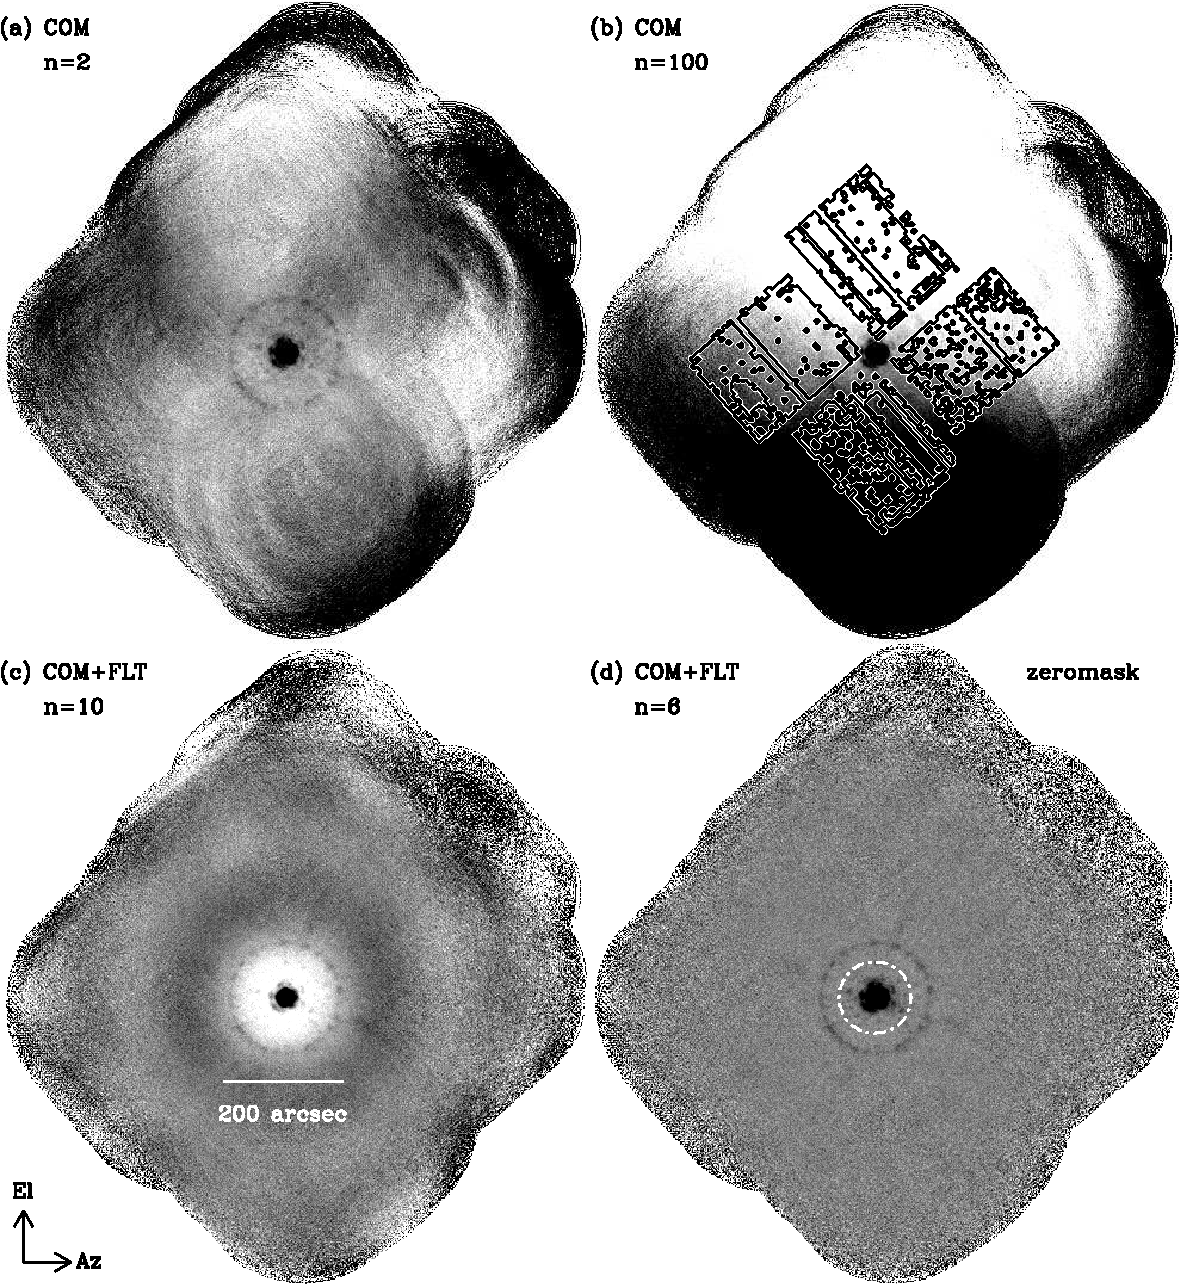
\includegraphics[width=\linewidth]{pointmaps.pdf}
\caption{Multiple reductions of a 450\,\micron\ constant-velocity
  daisy scan of Uranus, all scaled between $-$0.002\,pW (white) and
  +0.002\,pW (black). (a) Reduction in which only common-mode
  subtraction is used to suppress low-frequency noise, and the
  reduction is forced to use 2 iterations (after the first iteration
  an estimate of the source flux is removed, and the noise is measured
  in the residuals to obtain appropriate weighting for the second and
  final iteration). Circular streaks are caused by independent
  low-frequency noise that is not removed by the common-mode (Uranus
  peak 0.15\,pW). (b) Same as (a) but using 50 iterations,
  illustrating the degeneracy between large-scale structure and the
  common-mode (the footprint of working bolometers is also shown for
  reference, Uranus peak 0.15\,pW). (c) Reduction in which high-pass
  filtering above 0.775\,Hz (corresponding to a spatial scale of
  200\,arcsec as indicated) is applied after common-mode removal, but
  before the map estimate. The map-based convergence test is activated
  and the solution halts after 10 iterations, but leaving large-scale
  ringing due to the filter (Uranus peak 0.27\,pW). (d) Same as (c),
  but now the region of the map beyond the white dot-dashed circle is
  constrained to a value of zero until all but the final iteration.
  The map is now extremely flat, there is little attenuation of the
  source flux, and the diffraction pattern is clearly seen (Uranus
  peak 0.27\,pW).}
\label{fig:pointmaps}
\end{figure*}

\begin{figure}
\centering
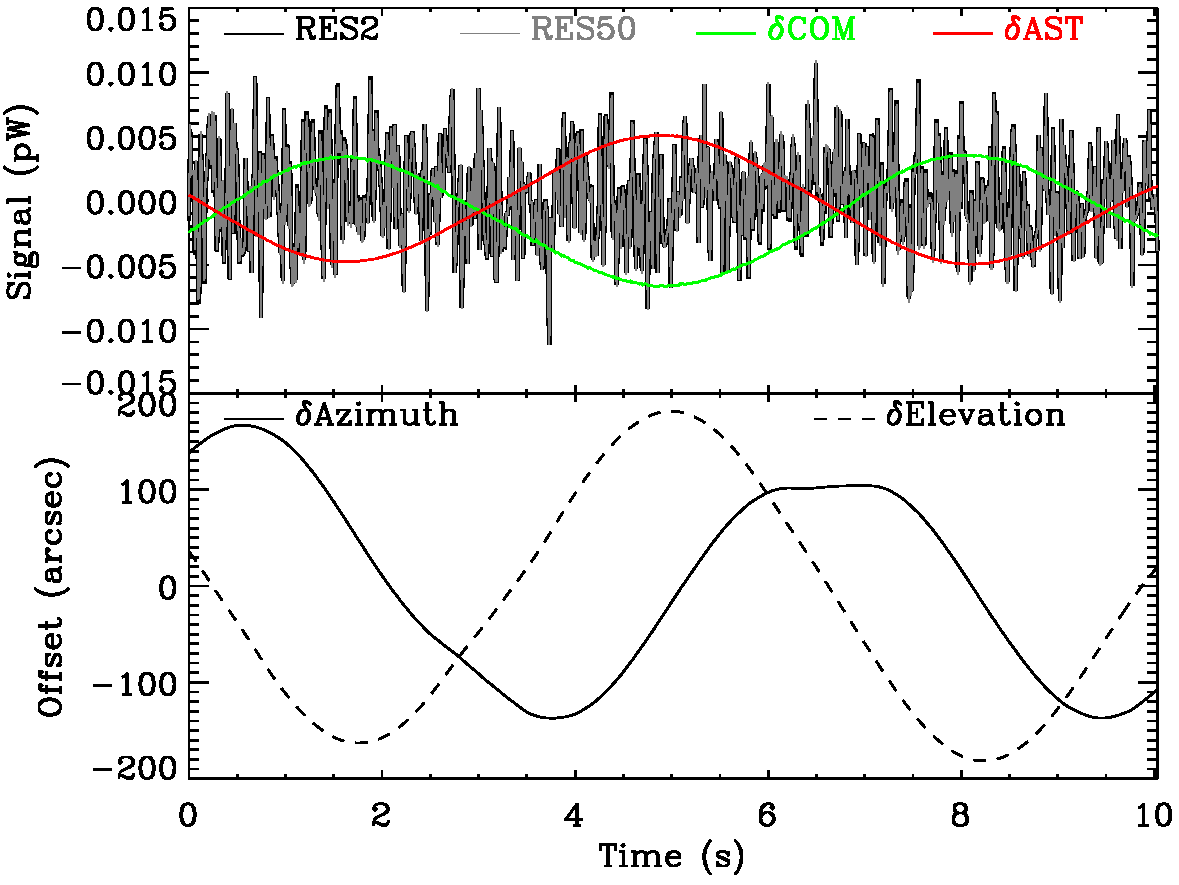
\includegraphics[width=\linewidth]{degeneracy.pdf}
\caption{Demonstration of the degeneracy between large-scale
  structures in the map and common-mode removal, corresponding to
  panels (a) and (b) in Fig.~\ref{fig:pointmaps}. The black and grey
  lines in the top panel show the residual signal for a single
  bolometer after 2 and 100 iterations, respectively (they are nearly
  identical; the black line lies beneath the grey line). The green and
  red lines show the difference between the \model{COM} and
  \model{AST} (the signal produced by the current map estimate for a
  given bolometer) model components for that bolometer between
  iterations 2 and 100, respectively. This shows that a strong signal
  has grown over time, and it has equal but opposite signs in the two
  model components, so that they cancel one another. The bottom panel
  shows the scan pattern of the telescope over the same period;
  clearly the \model{COM}/\model{AST} model degeneracy is correlated
  with the elevation offset, and referring to
  Fig.~\ref{fig:pointmaps}, panel (b), this corresponds to the strong
  vertical gradient that has appeared}.
\label{fig:degeneracy}
\end{figure}

%-------------------------------------------------
\subsection{Deep blind survey}
\label{sec:cosmo}
%-------------------------------------------------

\scuba\ surveys designed to detect extremely faint point-sources
(e.g., high-redshift star-forming galaxies, and debris disks) are
ideally limited by the white-noise performance of the instrument. The
approach described here for maximizing the \snr\ of point-sources
involves three major steps: (i) generating a map that removes most
low-frequency noise sources with approximately linear response,
without prior knowledge of the location of sources; (ii) whitening
(essentially flattening) the map to make the noise properties of the
map easier to deal with; and (iii) detecting point sources using a
``matched filter''. Note that variations on this general procedure
have been used extensively in the submm cosmology community using
previous instruments
\citep[e.g.,][]{scott2002,borys2003,laurent2005,coppin2006,scott2008,perera2008,devlin2009}.
In this section we will reduce scans of the Lockman Hole taken during
S2SRO as a pilot project for the Cosmology Legacy Survey. It consists
of $\sim8.5$\,hours of data taken in 36 separate scans (average
15\,min. each) spread over February and March 2010, covering an area
of about 50\,arcmin$^2$. The full list of dates and observation
numbers includes: 20100218, 63, 64, 65, 70, 71, 72, 90, 91, 92, 97,
98, 99; 20100220, 111, 112, 113, 118, 128, 129, 130; 20100303, 61, 62,
64, 69, 70, 72, 73, 74, 75; 20100309, 87, 88, 90, 91; and 20100311,
59, 64, 65, 72. These observations represent about 80 per cent of the
total data taken as part of the project; the remaining observations
were dropped due to problems keeping the arrays properly tuned during
S2SRO, and were easily identified by their highly variable and erratic
bolometer time-series (which resulted in maps full of large streaks).


\begin{figure*}
\centering
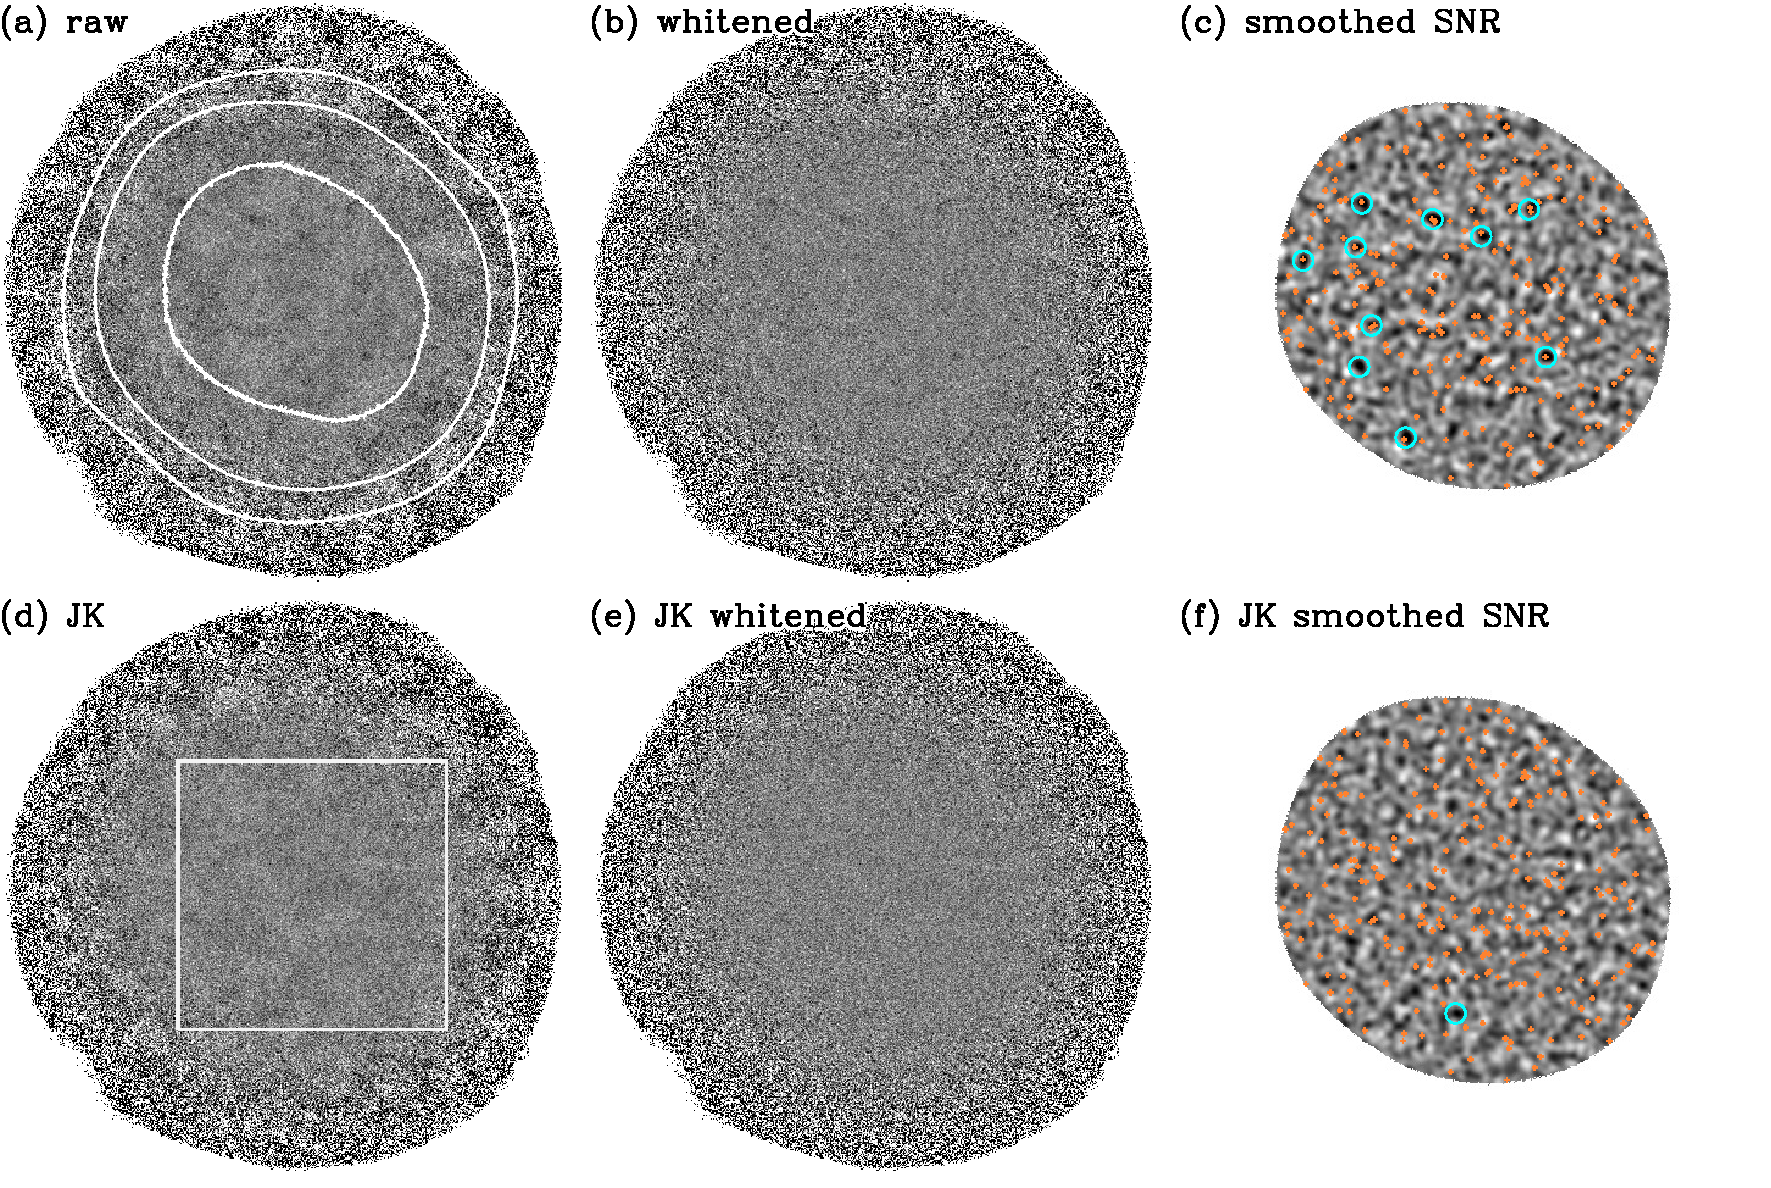
\includegraphics[width=\linewidth]{lockman_maps.pdf}
\caption{Reduction of a blank-field survey: the Lockman Hole. (a) Raw
  output of SMURF using high-pass filtering as a pre-processing step,
  followed by 4 iterations using only the \model{COM} model to remove
  residual low-frequency noise. White contours correspond to estimated
  noise levels of 1.25, 2.5 and 5.0 times the minimum noise at the
  centre of the map. (b) The whitened map using a filter based on the
  angular power spectrum of the jackknife map. (c) The whitened map
  cross-correlated with the whitened PSF to identify point sources
  [restricted to a lower-noise region, within the area denoted by the
  second contour of panel (a)]. The image shows the \snr\, with
  3.8-$\sigma$ peaks indicated with blue circles (radius
  8\,arcsec). The orange ``$+$'' signs show the locations of 1.4\,GHz
  radio sources from \citet{owen2008} with $S\gsim15$\,$\mu$Jy. Of the
  10 submm peaks, 9 are within this search radius of at least one
  radio source. (d) Jackknife map produced from the difference of two
  maps, using the even and odd scan numbers, respectively. Provided
  that all noise sources are statistically uncorrelated between the
  two halves of the data, the map is a plausible realization of the
  noise without contamination from astronomical sources. (e) The
  jackknife map whitened using the same filter as that in panel
  (b). The whitened jackknife map cross-correlated with the same
  whitened PSF as in panel (c). Again, orange ``$+$'' and blue circles
  indicate radio sources and 3.8-$\sigma$ peaks, respectively. Unlike
  panel (c), there is only a single (apparently) significant peak, and
  it is not in the vicinity of a radio source.}
\label{fig:lockman_maps}
\end{figure*}

The first step, map generation, is different from that described in
Section~\ref{sec:point} in two key ways. Since the locations of
sources are unknown \emph{a priori}, a map constraint is not
employed. Large-scale diverging structures in the map must be
mitigated, and the method used in this example (the default processing
in SMURF) is to apply a high-pass filter to the data once as a
pre-processing step. The iterative solution is then run using only
\model{COM}, \model{EXT}, \model{AST}, and \model{NOI}. In other
words, there is no information in the bolometer signals below some
cutoff frequency, and residual correlated high-frequency noise above
the cutoff is only removed through iterative common-mode
subtraction. The map is shown in Fig.~\ref{fig:lockman_maps}a. The
map-maker has been tested in two ways: (i) large numbers of iterations
are used to verify that the maps converge without the growth of large
structure; and (ii) adding synthetic sources to the data at a range of
brightnesses verify that the map-maker response to them is linear
(i.e., the relative shape and amplitude compared to the input source
is independent of brightness). The response to a synthetic point
source (solid line) after map-making (dotted line) is shown in
Fig.~\ref{fig:lockman_psf}. Clearly the use of a high-pass filter as a
pre-processing step, and having no other map-constraints, has the
down-side of introducing sidelobes around the main peak. However, the
way this filter affects point-sources is both well-known, and linear.

\begin{figure}
\centering
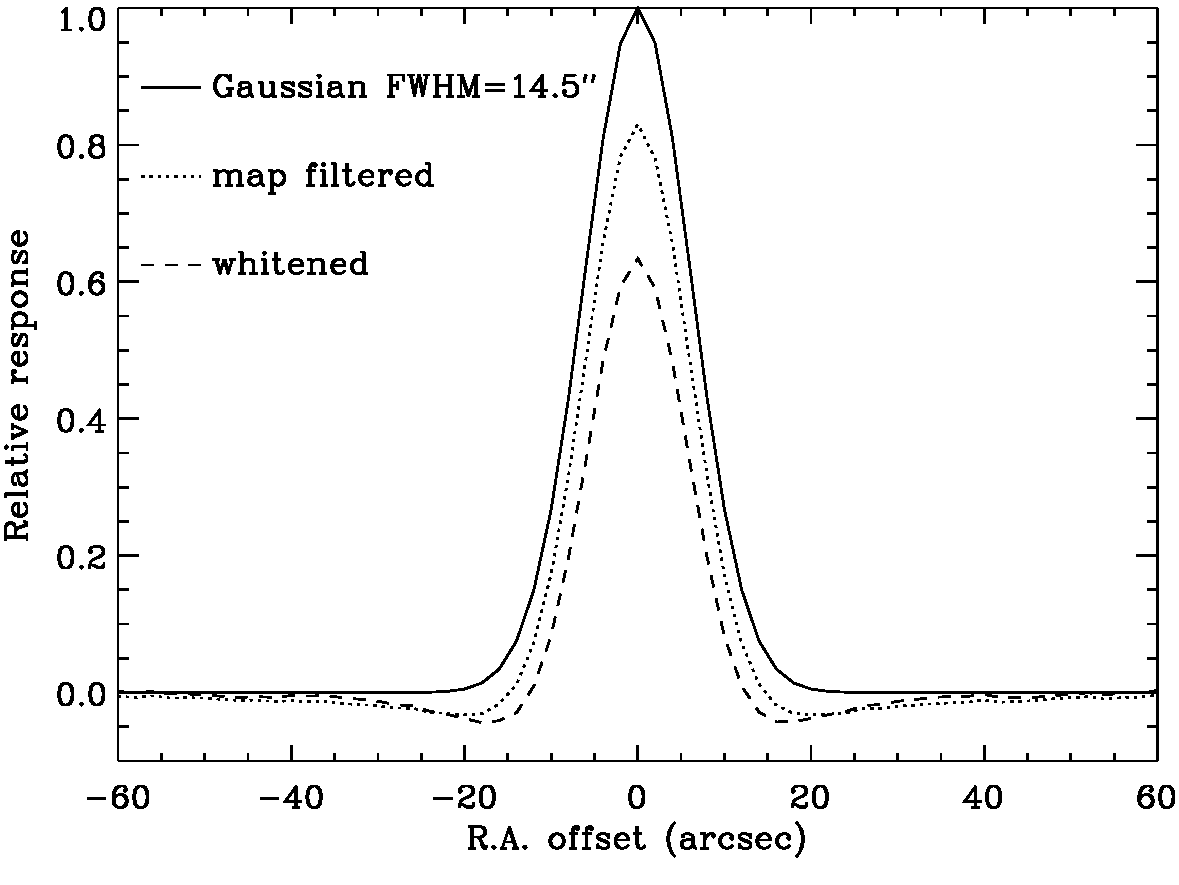
\includegraphics[width=\linewidth]{lockman_psf.pdf}
\caption{Slice through the angular response to an ideal Gaussian point
  source (solid line) along the R.A. axis following map-making using
  the default blank-field processing with SMURF (dotted line), and
  upon application of the whitening filter (dashed line). The ``map
  filtered'' response is produced by adding the ideal Gaussian to the
  real data near the centre of the Lockman Hole map, and re-reducing
  the data. The resulting dotted line gives the expected shape of a
  source in panel (a) from Fig.~\ref{fig:lockman_maps}. Applying the
  whitening filter (reciprocal of the solid orange line in
  Fig.~\ref{fig:lockman_pspec}) to the dotted line gives the whitened
  line, which is the expected shape of a source in panel (b) from
  Fig.~\ref{fig:lockman_maps}. Finally, cross-correlating the whitened
  map with this whitened PSF is an effective ``matched filter'' for
  identifying point-like sources, and this smoothed map is shown in
  panel (c) of Fig.~\ref{fig:lockman_maps}.}
\label{fig:lockman_psf}
\end{figure}

Even though the map looks quite flat, there is a mixture of faint
astronomical sources, and what is probably residual low-frequency
noise,q causing faint ripples visible to the naked eye. Since the
mixture of the two components is unknown, the first step is to
suppress the low-frequency noise, under the assumption that such
contaminants occur randomly in time, while astronomical sources are
(usually) constant.

First, the angular power spectrum of noise is estimated from a
``jackknife map'': maps are produced from two independent halves of
the total data set, and the jackknife signal in a map pixel,
$S_\mathrm{JK}$, and its variance, $\sigma^2_\mathrm{JK}$ are
estimated from the two input map fluxes, $S_1$, $S_2$, and the
corresponding variances, $\sigma^2_1$, and $\sigma^2_2$ as,
%
\begin{eqnarray}
S_\mathrm{JK} = \frac{S_1 - S_2}{2}, \\
\sigma^2_\mathrm{JK} = \frac{\sigma^2_1 + \sigma^2_2}{4}.
\end{eqnarray}
%
Provided that the noise in one half of the data is uncorrelated with
that from the other half, the signal in the jackknife map should
resemble noise drawn from the same parent distribution as that of the
real map. The astronomical signal, however, should be cleanly removed
(provided that there are no strong time-varying signals, and also
assuming that errors due to calibration between the two halves are
insignificant). The approach we have taken to minimize systematics is
to produce the two maps using odd and even scan numbers (i.e., each
map will contain a nearly evenly-spaced sampling of data across the
full data set).

Since the \scuba\ scan strategy is usually isotropic (all position
angles scanned with roughly equal weights), we make the simplifying
assumption that the angular noise power spectrum is azimuthally
symmetric. For these data, there are no obvious anisotropic structures
in the 2-dimensional FFT. The radial (azimuthally-averaged) angular
power spectrum therefore encodes all of the useful information about
the noise properties. These power spectra for the raw output of SMURF,
and the jackknife map (transforming only the approximately uniform
region indicated by the square in Fig.~\ref{fig:lockman_maps}d in each
case) are shown by the dashed black, and solid orange lines in
Fig.~\ref{fig:lockman_pspec}, respectively. Both power spectra are
approximately flat at spatial frequencies $\gsim 0.06$\,arcsec$^{-1}$
(scales $\lsim16$\,arcsec), with the exception of a line at
$\sim0.175$\,arcsec$^{-1}$ (a scale of $\sim5.7$\,arcsec). One
possibility for this feature is that it is related to the
inter-bolometer spacing in the focal plane (which happens to be this
size): small relative drifts in the baselines of adjacent bolometers
may produce faint parallel stripes in the map along the scan direction
(the superposition of many scans at different angles then results in
an isotropic noise pattern). It is not likely that this signal is due
to astronomical sources because it appears with a nearly equal
amplitude in both the real map and the jackknife.  At lower spatial
frequencies, both the real map and the jackknife power spectra grow
significantly, as a result of the more obvious large-scale undulations
in Figs.~\ref{fig:lockman_maps}(a) and (d).

\begin{figure}
\centering
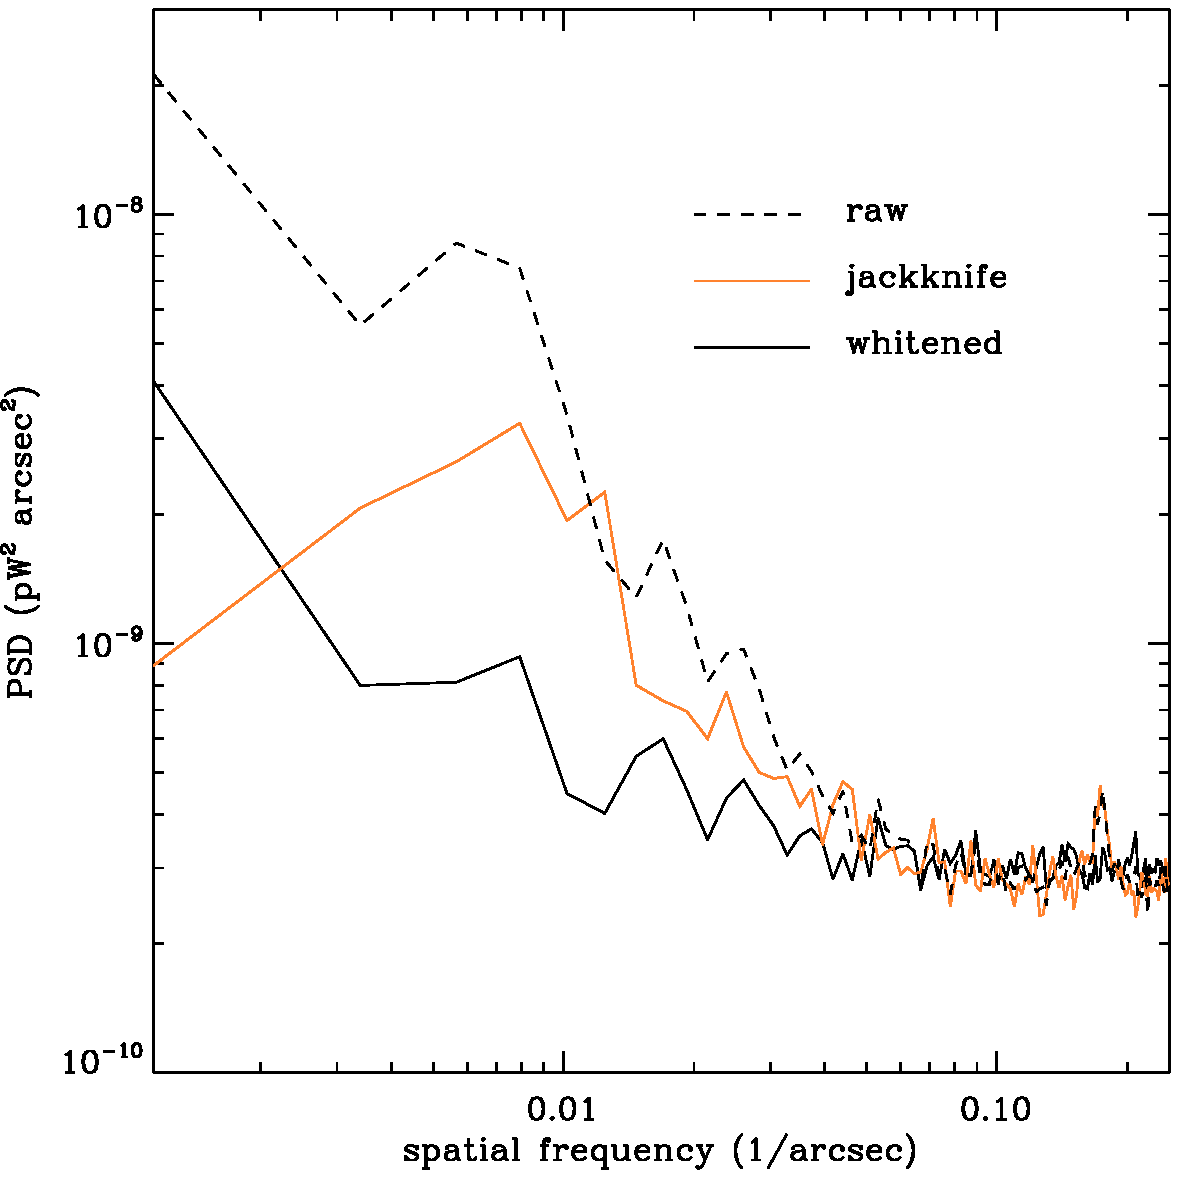
\includegraphics[width=\linewidth]{lockman_pspec.pdf}
\caption{Radial (azimuthally-averaged) angular power spectral
  densities for the raw map output by SMURF (dashed black line), the
  jackknife (solid orange line), and whitened (solid black line) maps
  (panels (a), (d), and (b) from Fig.~\ref{fig:lockman_maps},
  respectively, considering only the square region indicated in
  Fig.~\ref{fig:lockman_maps}d. Since the raw map contains spatially
  correlated signals on large scales, both due to noise and
  astronomical signals (low-spatial frequencies), the jackknife map
  (difference of two approximately equal-length subsets of the data)
  is used to generate a plausible realization of pure noise. Assuming
  that the noise properties are isotropic, a whitening filter is
  estimated from the reciprocal of the jackknife power spectrum with
  only a radial dependence. The power spectrum of the resulting signal
  map still has residual power on large scales, which is presumably
  due to astronomical sources.}
\label{fig:lockman_pspec}
\end{figure}

To suppress noise in the map, we construct a whitening filter from the
reciprocal of the jackknife angular power spectrum (orange line in
Fig.~\ref{fig:lockman_pspec}), normalised by the white-noise level
estimated from the RMS power at angular frequencies $>
0.1$\,arcsec$^{-1}$. The filter is applied by scaling the power
spectrum of the map by this function, and then transforming back into
real space. The whitened map is shown in Fig.~\ref{fig:lockman_maps}b,
and for comparison, the jackknife map has also been whitened in
Fig.~\ref{fig:lockman_maps}e. In both cases, the maps are visually
flatter than the non-whitened cases.

The angular power spectrum of the whitened signal map is shown with a
solid line in Fig.~\ref{fig:lockman_pspec}. At low angular frequencies
($\lsim 0.5$\,arcsec$^{-1}$) there is significantly less power than
the raw map. However, it also clearly has some power in excess of the
white noise level. In theory, this residual signal is produced by
astronomical sources, although its origin cannot be determined from
this plot alone; nor are astronomical sources readily visible in the
map (Fig.~\ref{fig:lockman_maps}b). To identify sources, we next apply
a matched filter to the whitened maps.

For blind, high-redshift surveys, individual sources are expected to
be un-resolved by the \scuba\ 7.5--14.5\,arcsec FWHM beams. Under this
assumption, cross-correlation between the map and the known PSF yields
the maximum-likelihood flux density of supposed point-sources centered
over every location in the resulting map \citep[an extremely
well-known result throughout astronomy, see][]{stetson1987}. Peak
identification in such smoothed maps have been used extensively in the
submillimetre community as both an efficient source-detection and
photometric measurement strategy. In terms of the angular power
spectrum, a matched filter may also be thought of as an optimal
low-pass filter, that suppresses noise on scales smaller (and
therefore higher angular frequencies) than the beam. For the case at
hand, the effective PSF for the whitened maps is given by the dotted
curve in Fig.~\ref{fig:lockman_psf}. Maps smoothed by this shape are
shown for the whitened signal, and jackknife maps in
Figs.~\ref{fig:lockman_maps}c and f, respectively. Note that these
images are plotted in \snr\ units, where the smooth noise maps have
been calculated by propagating the original noise maps output by SMURF
both through the whitening and matched filters (each of which are
linear operations).

Have real astronomical sources been detected using the matched filter?
For both the smoothed signal and jackknife maps, orange circles denote
3.8-$\sigma$ peaks. While not justified here, this threshold is fairly
typical for other ground-based submillimetre surveys in recent years
\citep[e.g.,][]{coppin2006,perera2008,2009ApJ...707.1201W} leading to
estimated false-identification rates of order $\sim$5\%, and is chosen
as a convenient reference. In the former, 10 peaks are found, whereas
there is only 1 in the latter. However, this test does not preclude
the possibility that some correlated noise made it into the jackknife
map, in which case the estimated \snr s are misleading.

One simple test of the calculated noise properties is to compare the
signal and jackknife \snr\ distributions with ideal Gaussians. The top
panel of Fig.~\ref{fig:lockman_hist} shows the whitened (but not
match-filtered) signal (blue) and jackknife (histograms), along with a
Gaussian (mean 0, standard deviation 1, and area normalised to the
number of map pixels) as a dashed line. In this case, it is clear that
the \snr\ distributions for both maps are nearly indistinguishable
from the theoretical distribution of white noise. This result shows us
that: (i) the whitening filter appears to have removed correlated
large-scale noise, since the jackknife map histogram is consistent
with white noise; and (ii) any potential astronomical signals are
small compared to the typical white noise in most map pixels
(unsurprising given the appearance of
Fig.~\ref{fig:lockman_maps}b). Next, we examine the \snr\ histograms
for maps processed with the matched filter in the bottom panel of
Fig.~\ref{fig:lockman_hist}. Again, the histogram of the jackknife
\snr\ data appears consistent with pure noise. However, the signal map
now deviates significantly from a Gaussian distribution, with a clear
positive tail (as one would expect for emitting sources). In fact,
integrating the positive tails beyond our 3.8-$\sigma$
source-detection threshold (vertical solid line) yields 229 map pixels
in the signal map, compared with 3 in the jackknife map (out of 80603
pixels in the entire region). Recall that given the small pixel size
of the map, several pixels generally contribute to each peak. Note
that this procedure gives only a flavour of the analysis that is
usually required to produce a robust source lists. Additional tests,
along with a careful consideration of completeness and false-positive
rates usual require a series of Monte Carlo simulations that are
beyond the scope of this work. We direct the interested reader to a
selection of papers on the subject:
\citet{scott2002,coppin2006,perera2008,2009ApJ...707.1201W} and
\citet{chapin2011}.

\begin{figure}
\centering
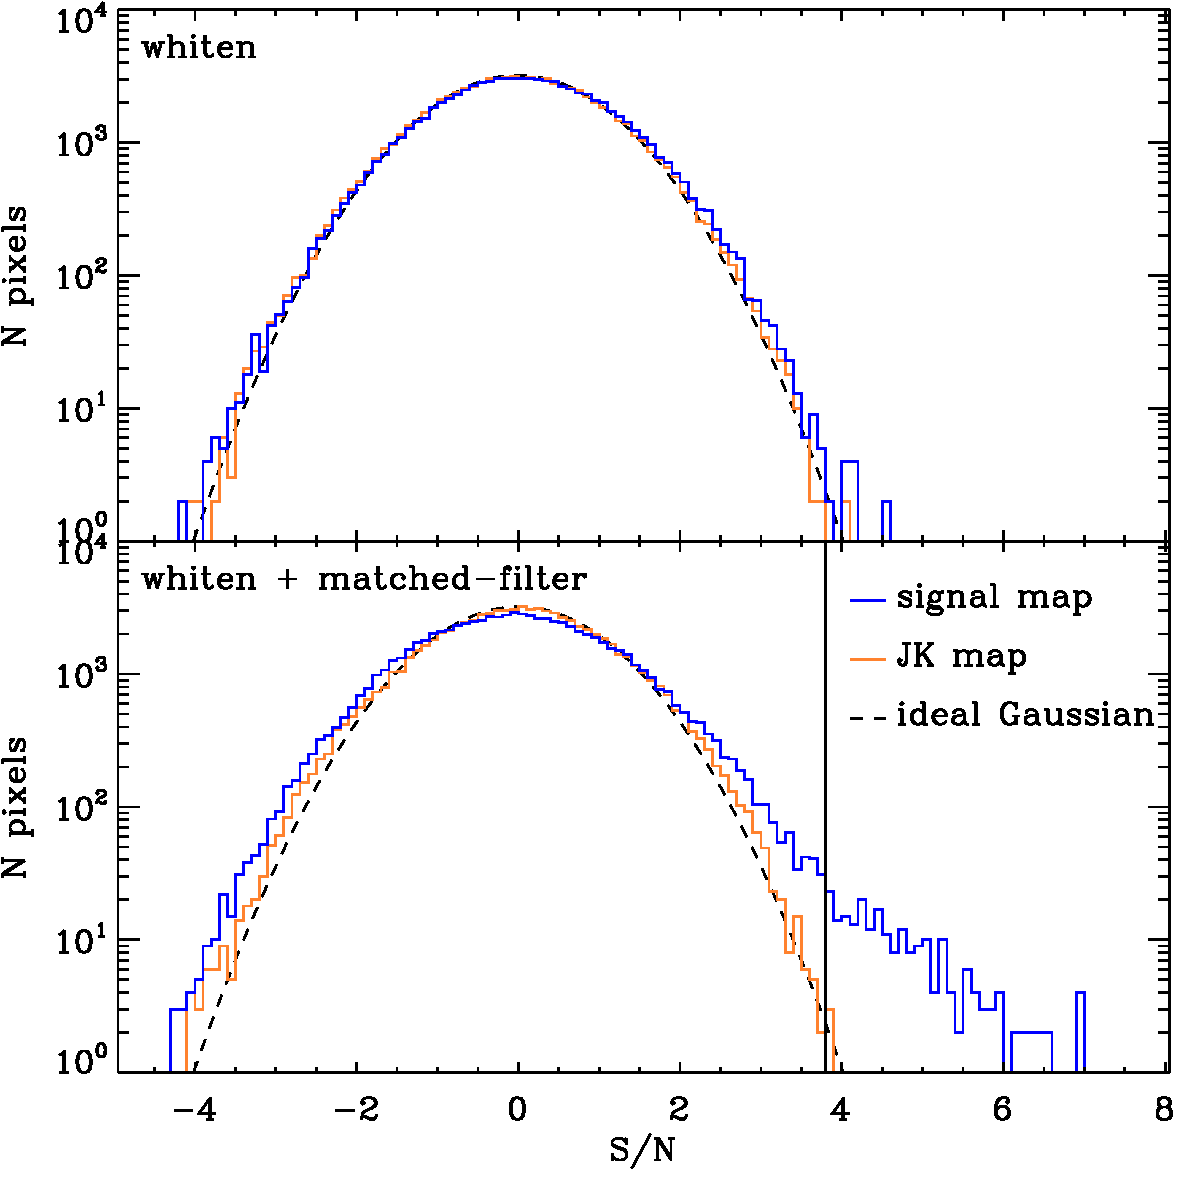
\includegraphics[width=\linewidth]{lockman_hist.pdf}
\caption{Histograms of \snr\ using pixels from the central region of
  the Lockman Hole (second contour) in
  Fig.~\ref{fig:lockman_maps}a. The top panel shows the histograms for
  pixels from the whitened signal and jackknife maps
  (Figs.~\ref{fig:lockman_maps}b,e), compared to a Gaussian
  distribution with mean zero, standard deviation one, and an area
  normalised to the total number of pixels -- the expected
  distribution for a map of spatially-uncorrelated Gaussian noise. The
  good agreement indicates that these maps are indeed dominated by
  white noise. The lower panel shows the results for matched filtered
  signal and jackknife maps (Figs.~\ref{fig:lockman_maps}c,f). The
  filtered jackknife map distribution is still close to the
  expectation (Gaussian), but now the matched filter has picked out
  significant signal, leading to the large positive tail. The vertical
  solid line shows the chosen 3.8-$\sigma$ source-detection
  threshold.}
\label{fig:lockman_hist}
\end{figure}

As an additional external check, we have over-plotted orange ``$+$''
signs at the locations of 1.4\,GHz radio sources from \citet{owen2008}
with $S\gsim15$\,$\mu$Jy. Such radio catalogues have historically
proven invaluable for the precise identifications of high-redshift
submillimetre galaxies due to their relatively low surface densities
(compare with optical catalogues, for example), and a strong
correlation between the radio and submillimetre emission mechanisms
\citep[e.g.,][]{smail2000,pope2006,ivison2007,chapin2009b}. Taking a
representative search radius of 8\,arcsec from these studies with
similar \snr\ sources and source sizes (the same size as the blue
circles), 9 out of 10 peaks in the smoothed signal map have potential
radio counterparts, whereas the single peak in the smoothed jackknife
map does not lie near any radio source. Again, a proper
cross-identification analysis must inevitably include simulations to
establish completeness, false-positive rates, as well as the effects
of point source clustering and confusion. See the aforementioned
papers and references therein for examples.

\begin{figure*}
\centering
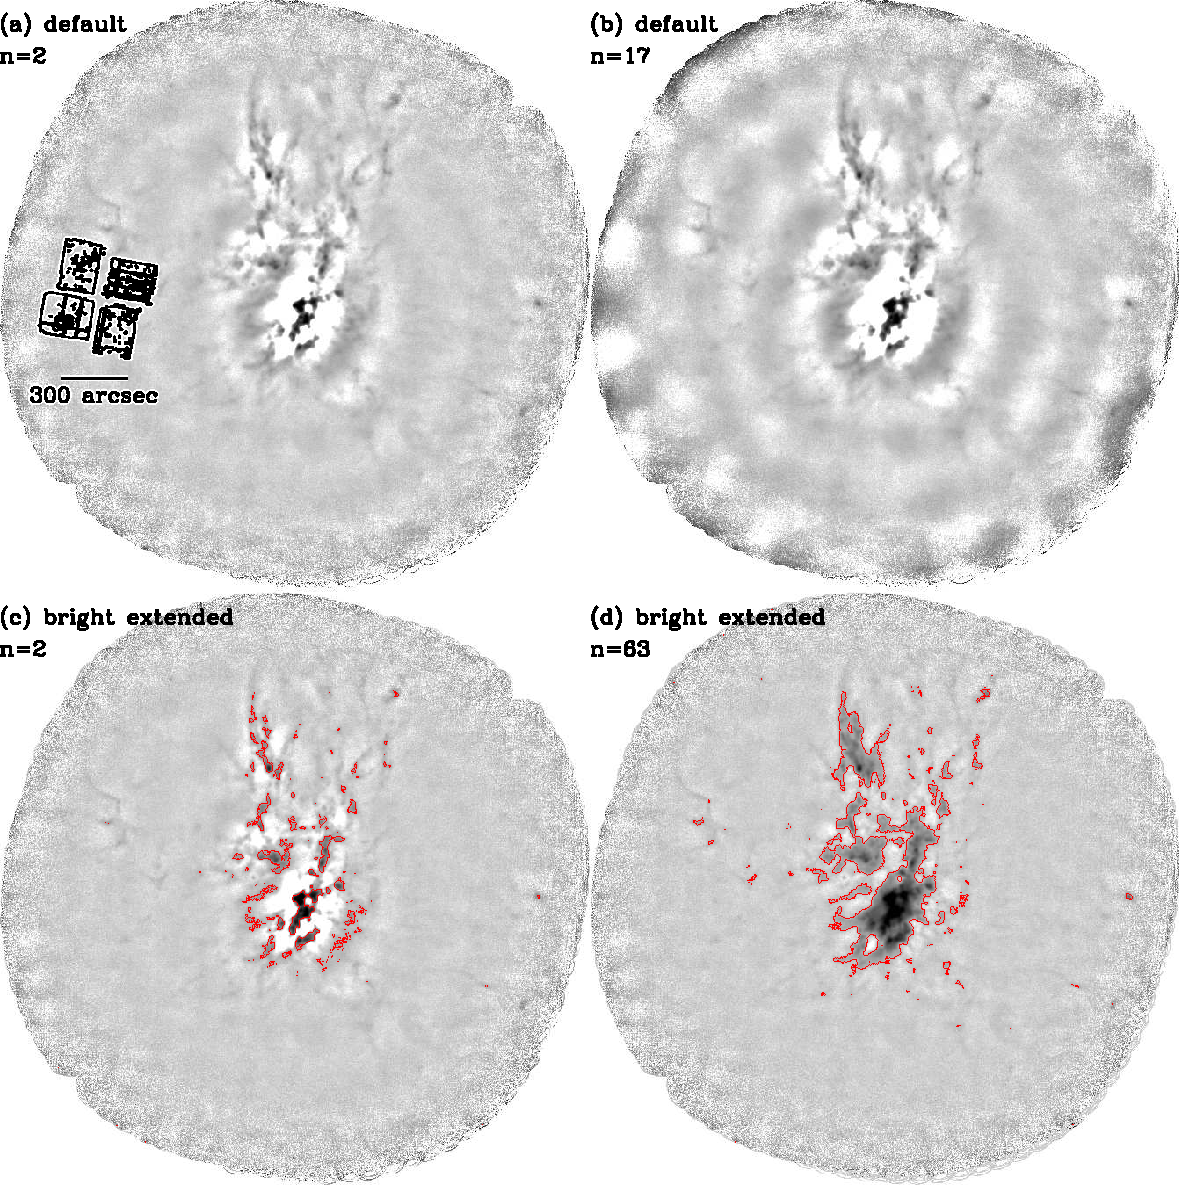
\includegraphics[width=\linewidth]{m17.pdf}
\caption{An 850\,\micron\ rotating PONG map of M17. Intensity is
logarithmically scaled between $-$0.0003\,pw (white) and +0.01\,pW
(black). Iteration numbers are given in the corner of each
panel. Panels (a) and (b) show the results for a reduction using the
default parameters (the solution halted after reaching the default
map-based convergence criterion in 30 iterations). Panel (a) also
depicts the array footprint (position angle indicative of the start of
the observation), and a 300\,arcsec line shows the spatial scale
corresponding to the default \model{FLT} high-pass filter. Similar to
Fig.~\ref{fig:pointmaps}c, the lack of prior constraints on the map
leads to degeneracies, and therefore ripples on scales larger than the
array footprint (due to common-mode subtraction) and filter scale
(especially evident around the brightest peak at the centre of the
map). Panels (c) and (d) show the ``bright extended'' reduction, in
which a zero-mask is created iteratively from all of the pixels that
exceed an \snr\ of 5. While this region (red contour) only encompasses
the brightest peaks early in the solution, in the final iteration it
identifies most of the bright, extended emission, and significantly
helps with negative ringing.}
\label{fig:m17}
\end{figure*}

For future, significantly deeper \scuba\ maps, in which the RMS in a
PSF-smoothed map is dominated by point-source confusion, rather than
instrumental noise, a modified matched filter will offer improved
results. See Appendix~A in \citet{chapin2011}, which shows how to
include confusion (when known \emph{a priori}) explicitly as a noise
term in the calculation of such filters.

%-------------------------------------------------
\subsection{Bright extended emission}
\label{sec:extended}
%-------------------------------------------------

In this final example, we analyze a map of M17 which contains bright,
extended emission, in contrast with the earlier two examples. A
promise of \scuba\ is to recover larger angular scales than what was
possible with earlier-generation ground-based submillimetre
cameras. The two main factors contributing to this expectation are:
(i) a larger array footprint on the sky which should make the
subtraction of common sky-emission signals more effective; and (ii)
fast detectors (with a correspondingly fast sample rate) to enable
higher slew-rates (up to 600\,arcsec\,s$^{-1}$) to capture as much
large-scale structure as possible above the detector $1/f$ knees. We
produce maps of observation 11 on 20110531 using the 850\,\micron\
array. It is a rotating PONG covering a diameter of 0.375\,deg, with a
scan speed of 300\,arcsec\,s$^{-1}$, and a transverse spacing of
180\,arcsec, taking 37.5\,min to complete.

The default reduction of these data is shown in the top panels of
Fig.~\ref{fig:m17}, after 2 iterations (the first map estimated after
the noise weights have been measured) and 17 iterations (when the map
has converged). The first panel also depicts the array footprint, and
the angular scale corresponding to the high-pass filter edge. Much
like the reduction of a point source without any prior constraints
(Fig.~\ref{fig:pointmaps}c), degeneracies on scales larger than the
array footprint and filter produce ripples in the map.

Unlike the case of a known point-source (Section~\ref{sec:point}), it
may not be possible for the observer to define, in advance, a mask of
regions containing blank sky. Indeed, for this map, much of the field
clearly contains extended structure. Furthermore, the goal of such
maps may be to detect previously unknown cool, dense regions of the
ISM that may not have appeared at other wavelengths (e.g., the first
optically-thick cloud-collapse stages of star-formation). While the
option does exist for the user to supply their own mask, a facility
has been added to SMURF to generate one automatically by flagging
pixels above some \snr\ threshold after each iteration as part of the
``bright extended'' configuration.

The results of this automatic masking are shown in the bottom panels
of Fig.~\ref{fig:m17}. After the second iteration, only narrow regions
around the brightest peaks are identified. However, as the solution
progresses, the negative bowls around the bright sources are slowly
reduced and the mask ``grows'' out from the brightest areas. By the
final iteration, most of the obvious structures in the data are
encompassed by the mask, negative bowling is significantly reduced,
and the brightest regions are clearly more extended.


\begin{figure*}
\centering
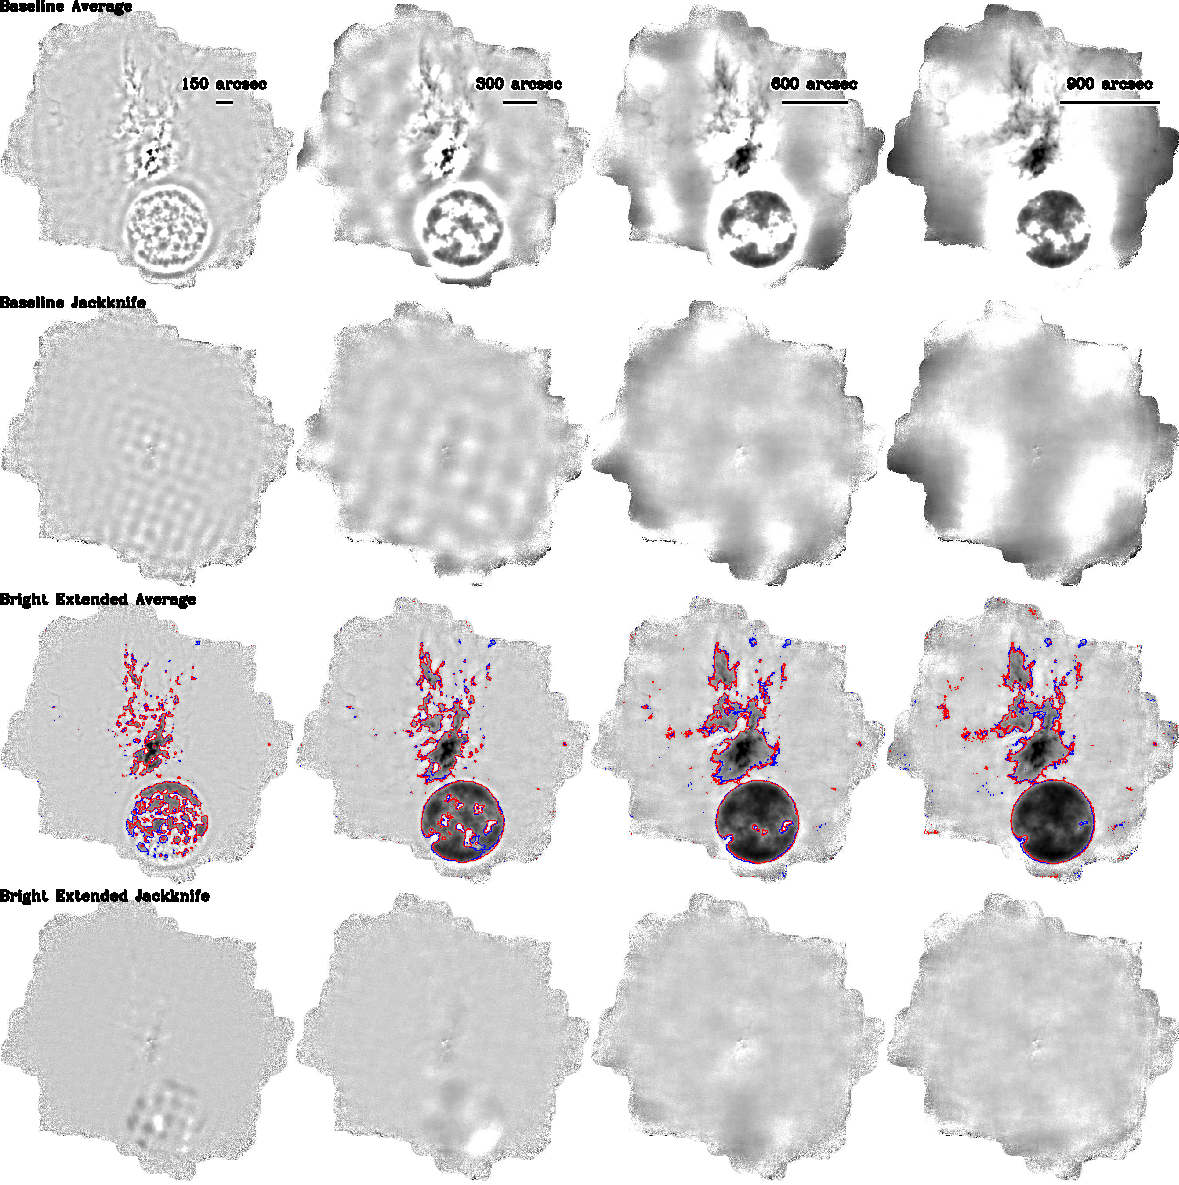
\includegraphics[width=\linewidth]{m17_jk.pdf}
\caption{Maps of M17 used to characterize the noise properties and
transfer function of SMURF (same intensity scale as
Fig.~\ref{fig:m17}). For each column, a different high-pass filter
edge scale was adopted (indicated in the top panels). First (top) row:
average of two halves of the data analysed independently, using the
default configuration. The data have had added to them synthetic
signal within a 600\,arcsec diameter circle (south of M17) created as
a realization of noise from a $P(k) \propto k^{-3}$ angular power
spectrum multiplied by the PSF, subtracting the minimum to make it
positive, scaling it to a similar signal range as M17 itself, and
rolling-off the edges smoothly using half a period of a radial
(1+cosine)/2 function across 100\,arcsec beyond the edge of the
600\,arcsec region. Second row: jackknife maps produced from the
differences of the maps of each half of the data that went into the
first row. Third row: average of the two halves of the data using the
bright extended reduction. The blue and red contours indicate the
zero-masked regions for each half of the data (note for the
300\,arcsec case that the region about M17 matches fairly closely the
mask in Fig.~\ref{fig:m17}d). Clearly as the filter scale is
increased, due to the high \snr\ of the data, larger emission regions
are (correctly) detected and reproduced in the map. Fourth (bottom)
row: Jackknife maps for the bright extended reductions.}
\label{fig:m17_jk}
\end{figure*}

\begin{figure*}
\centering
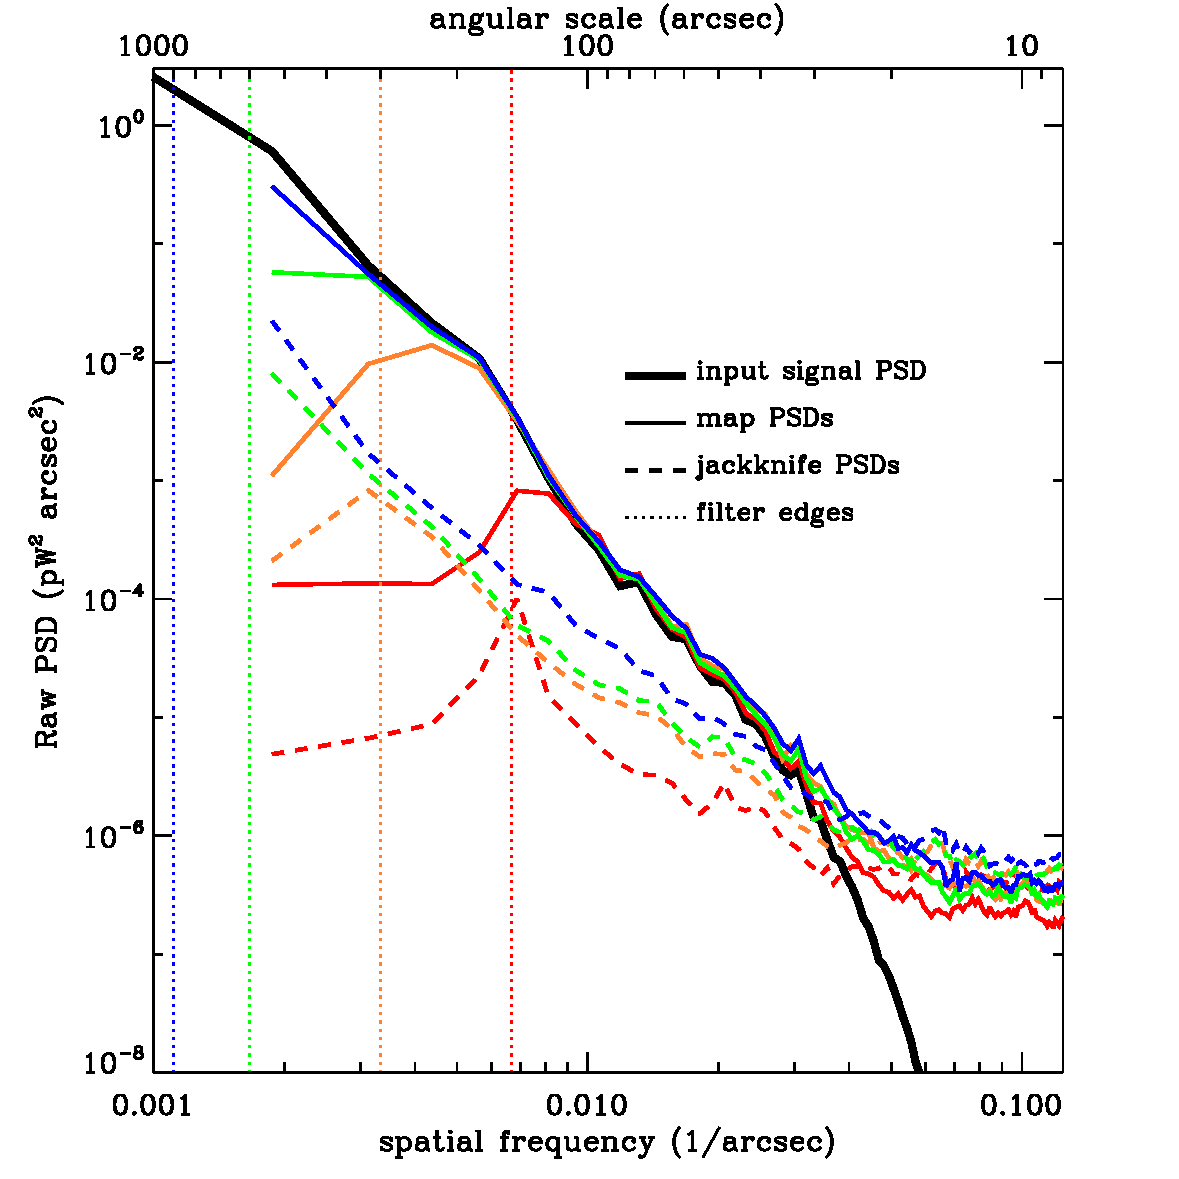
\includegraphics[width=0.49\linewidth]{pspec_m17_default.pdf}
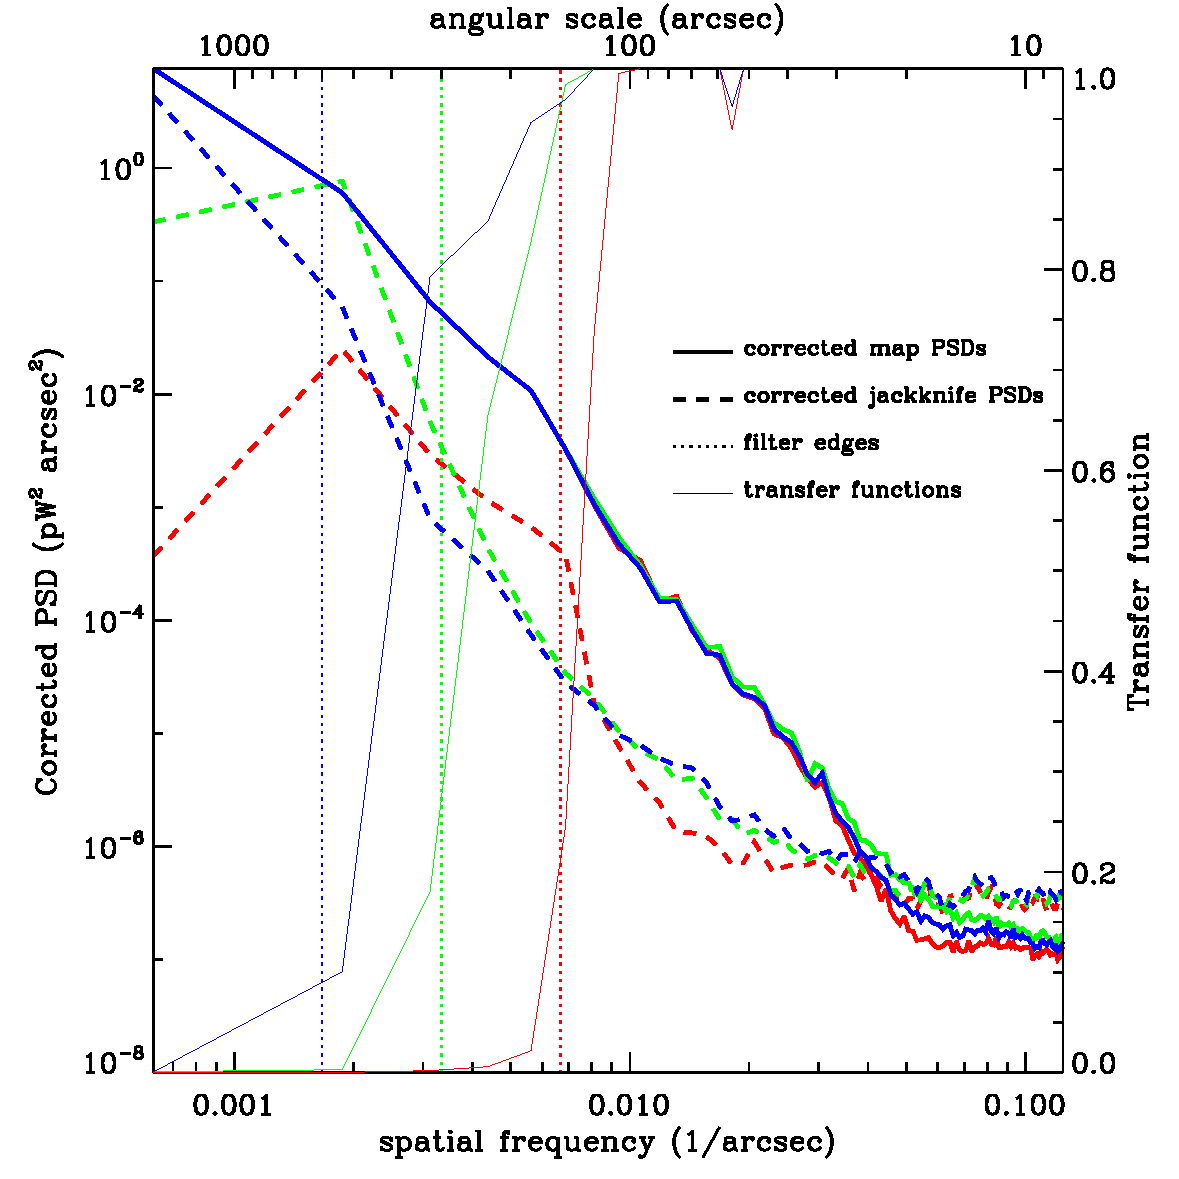
\includegraphics[width=0.49\linewidth]{cor_pspec_m17_default.pdf}
\caption{Angular power spectral densities (PSDs) for the region of the
M17 map in Fig.~\ref{fig:m17_jk} containing synthetic data, using the
default configuration. Left: raw PSDs for the input (noiseless)
simulated data (thick black line), the signal (average of each half)
PSDs (thin solid lines), and noise PSDs estimated from the jackknives
(dashed lines). Vertical dotted lines indicate the high-pass filter
scales: 150\,arcsec (red); 300\,arcsec (orange); 600\,arcsec (green);
and 900\,arcsec (blue). PSDs are also colour-coded by filter
scale. Right: since the input PSD is known, it is possible to measure
the transfer function of the map-maker as the ratio between the output
map signal PSDs and the input PSD (from the left panel), giving the
thin coloured lines (linear vertical axis shown on right of plot). The
remaining lines are as in the left panel, but now corrected by the
transfer function. This plot shows that increasing the filter scale
improves the \snr\ at intermediates scales ($\sim$200--600\,arcsec),
although the \snr\ worsens at smaller scales ($\lsim$200\,arcsec).}
\label{fig:m17_def_ps}
\end{figure*}

\begin{figure*}
\centering
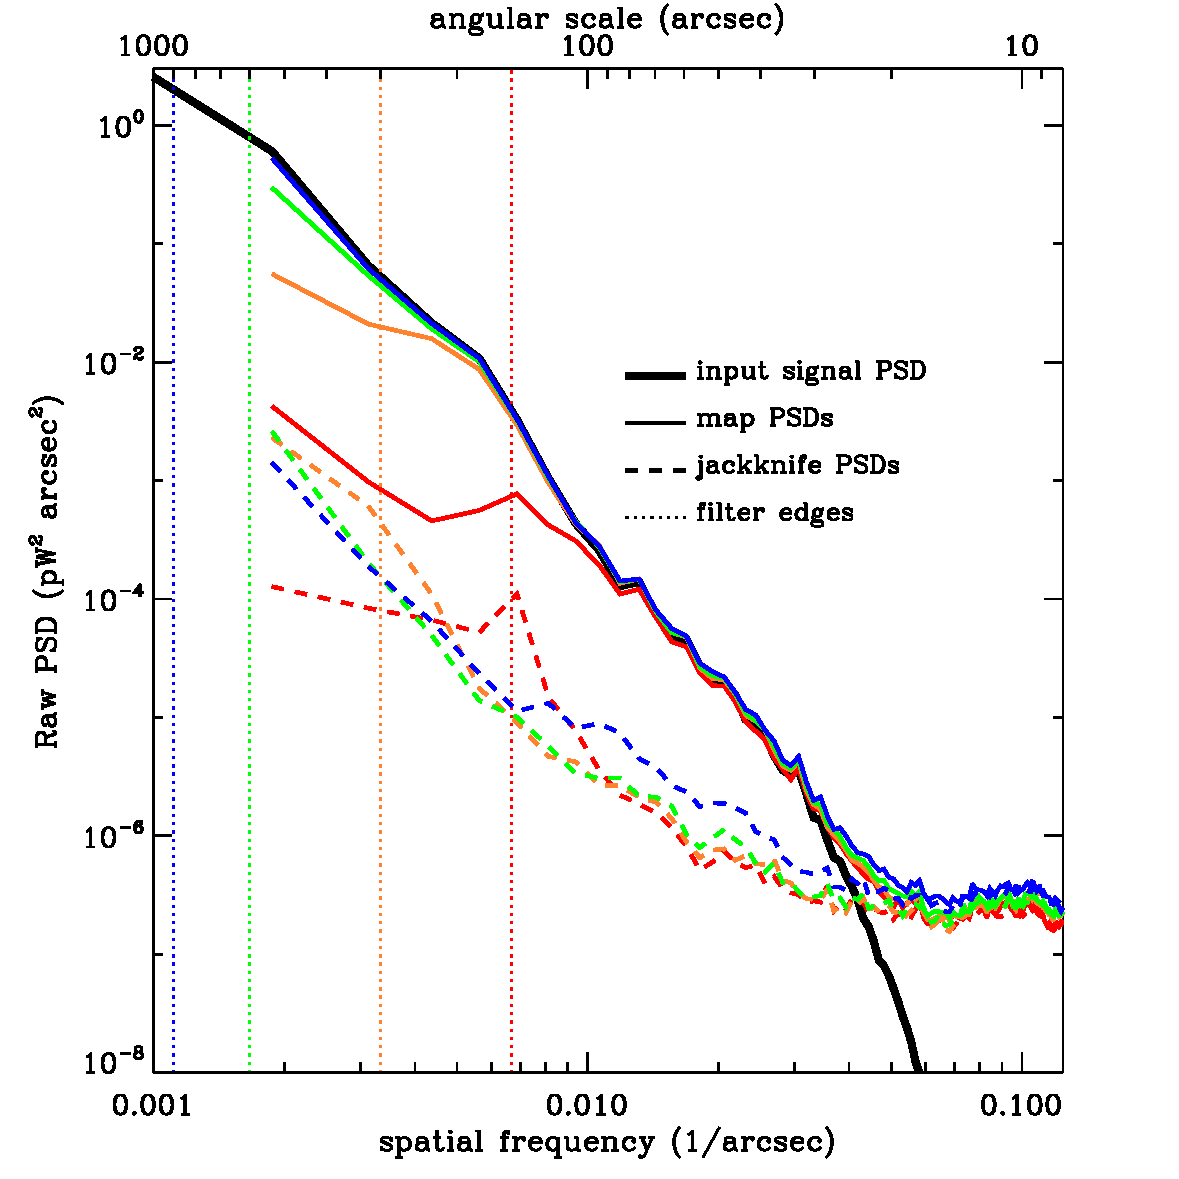
\includegraphics[width=0.49\linewidth]{pspec_m17_bright_extended.pdf}
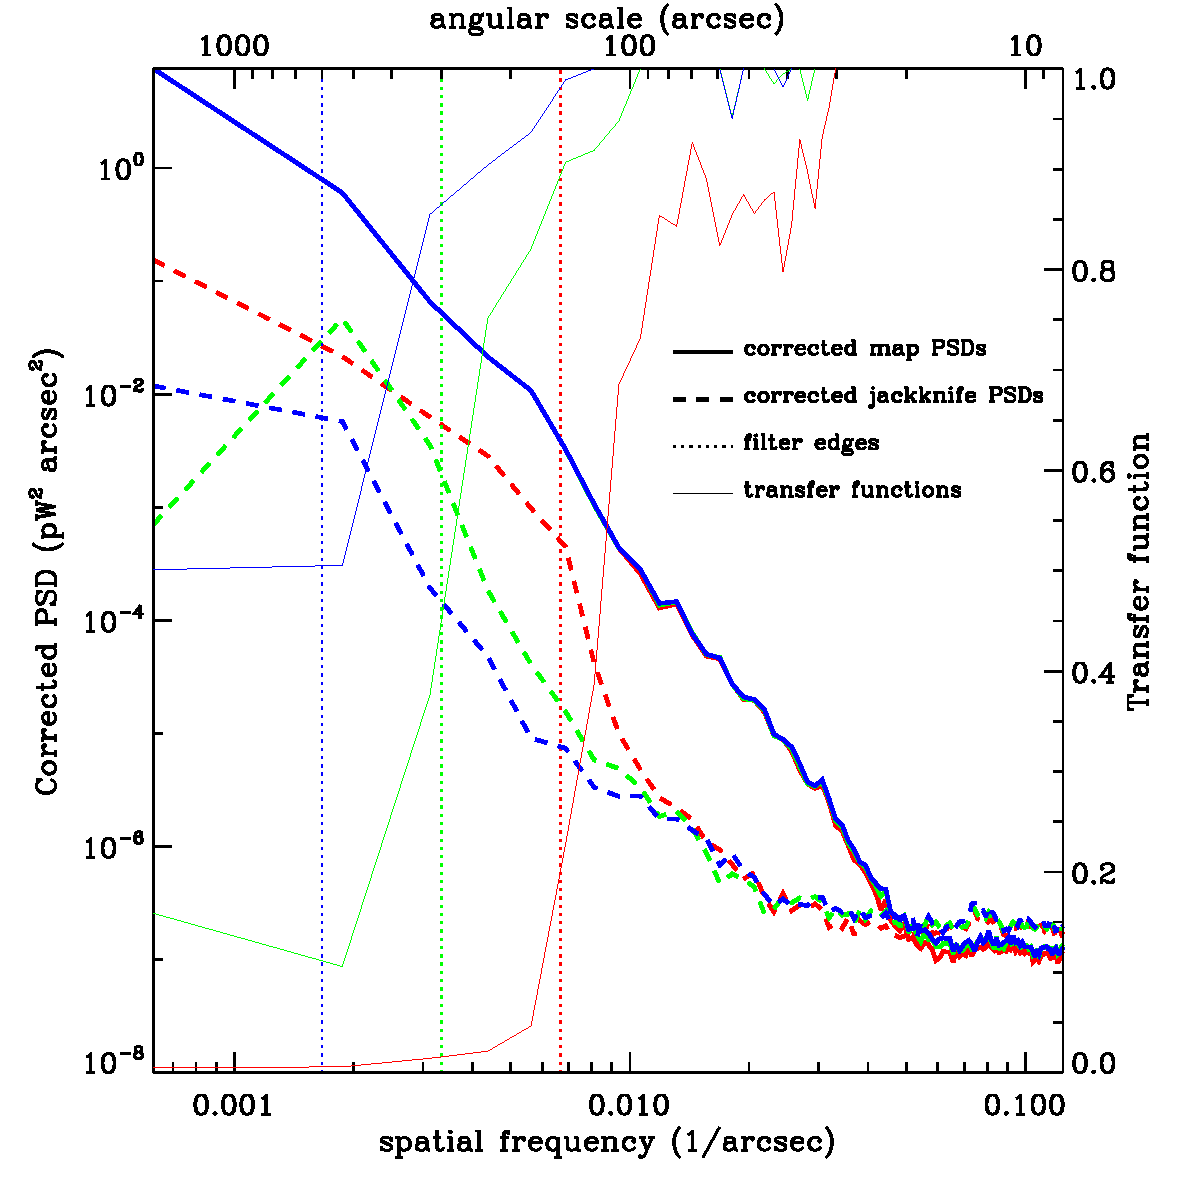
\includegraphics[width=0.49\linewidth]{cor_pspec_m17_bright_extended.pdf}
\caption{Lines have same meaning as in Fig.~\ref{fig:m17_def_ps},
except now using the bright extended configuration. This configuration
has resulted in an improved transfer function and \snr\ at large
angular scales. Also note that increasing the filter scale does not
have as large an impact on the small-scale noise as in the default
configuration, although it is still noticeably larger up to scales of
about 60\,arcsec.}
\label{fig:m17_be_ps}
\end{figure*}

While the reduction in the bottom panels of Fig.~\ref{fig:m17} is
clearly superior, in at least a cosmetic sense to those in the top
panels, it is important to quantify both the noise properties of the
maps and their response to real structures (the transfer function). We
would also like to know how each are affected by our choice of filter
scale.  Similar to the previous section, we will use a jackknife test
to estimate the noise, as well as injecting known sources into the
data to observe how they are attenuated.

Maps are produced using the first and second continuous halves of the
data in Fig.~\ref{fig:m17_jk}. This is not an ideal situation, since
the noise properties may evolve with time (e.g., due to changing sky
conditions) leading to a biased estimate of the parent noise
distribution in the complete map from the jackknife. Also, since the
zero-masking depends on the \snr\ of the map, it will be restricted to
regions approximately $\sqrt{2}$ shallower in these maps than for the
full data set. Finally, the cross-linking (positional angles sampled)
is similar, though not identical in the two halves. Ideally one would
have many full maps, as in the case of the Lockman Hole data in the
previous section, from which alternating maps could be combined.

Since our goal in this section is to measure the response of the
map-maker to extended structures, we inject a simulated signal with
power at a range of scales into a relatively empty region of the map.
It is created by drawing a realization of noise within an 800\,arcsec
on-a-side box, with an angular power spectrum $P(k) \propto k^{-3}$
which is appropriate for Galactic cirrus clouds
\citep[e.g.,][]{gautier1992}. It is then filtered again with a
14.5\,arcsec Gaussian to model the effect of the \scuba\ optical
response. The RMS of these fluctuations is then normalised to 0.002 pW
so that they are comparable to the dynamic range of M17 itself. The
minimum is then subtracted so that the signal is positive. Finally,
half a period of a (1+cosine)/2 function is used to roll-off the
signal to zero between radii of 300 and 400 arcsec.

The first row of Fig.~\ref{fig:m17_jk} shows the total signal image
averaging the maps made of each independent half of the data, for the
default configuration (inverse-variance weighting has been used). The
columns show reductions using 150, 300, 600, and 900\,arcsec filter
edges in the reductions. For reference, the largest scale that is
completely inscribed by the array footprint is about 400\,arcsec, and
the diagonal of the array is about 600\,arcsec (meaning that scales
beyond 600\,arcsec are completely unconstrained when common-mode
rejection is used).  The synthetic data are clearly seen as the
circular region south of M17. As the filter scale is increased, the
size of the ripples increases accordingly. While larger structures do
seem to appear, negative bowls are a major problem without any other
map constraints.The second row of Fig.~\ref{fig:m17_jk} shows the
jackknife maps. The astronomical emission is almost perfectly removed,
except for a slight impression of M17 near the centre of the map, that
is probably due to some combination of detector gain and pointing
drifts. Otherwise the jackknife appears to be a plausible realization
of noise from the same parent distribution as for the averaged maps.

The third and fourth rows in Fig.~\ref{fig:m17_jk} repeat this
exercise using the bright extended configuration, in which the \snr\
threshold of 5 is again used to constrain the map. As the filter scale
is increased, more of the extended structure in M17 is reproduced in
the map, as evidenced by the blue and red contours (masks generated
from the first and second halves of the data, respectively). The
masking does a generally good job of suppressing the largest-scale
ripples that are produced by the default reduction. However, the noise
away from regions of bright emission does increase noticeably (mottled
appearance). With filter scales $\gsim600$\,arcsec, virtually the
entire region of synthetic emission is correctly identified by the \snr\
mask and allowed to vary freely in the solution.

Next, we analyse the angular power spectra densities (PSDs) of the
maps to understand the signal and noise properties of the map-maker in
the region of synthetic sources, as a function of filter scale. The
left panel of Fig.~\ref{fig:m17_def_ps} shows the raw PSDs for the
input synthetic signal (thick black line), the output map signals
(thin solid lines), and the jackknife maps (dashed lines). Colours
encode the filter scales used: 150\,arcsec (red); 300\,arcsec
(orange); 600\,arcsec (green); and 900\,arcsec (blue). Note that, with
the exception of the synthetic data, we only plot the PSDs down to the
second-lowest spatial frequency bin of
$1.875\times10^{-3}$\,arcsec$^{-1}$, or 533\,arcsec, due to the fact
that the smallest is very poorly sampled, and therefore noisy. As the
filter edge is increased, more power is measured in the map PSDs at
larger scales. However, much of this power is clearly produced by
noise which appears in the jackknife PSDs. We estimate the map-maker
transfer function as the ratio between the portion of the signal PSDs
not produced by noise, to the input PSD, or
%
\begin{equation}
G(k) = \frac{P_\mathrm{M}(k) - P_\mathrm{JK}(k)}{P_\mathrm{S}(k)},
\end{equation}
%
where $k$ is the spatial frequency, and the subscripts ``M'', ``JK'',
and ``S'' refer to the signal map, jackknife map, and synthetic map,
respectively.

The transfer functions $G(k)$ are plotted as thin solid lines in the
right panel of Fig.~\ref{fig:m17_def_ps}. This formula produces
extremely noisy values at large frequencies (small scales), and we
therefore set it to a value of 1 above 0.015\,arcsec$^{-1}$, as well
as any point in the curve where $P_\mathrm{M}(k)$ exceeds
$P_\mathrm{S}(k)$ (i.e., $G(K)$ is assumed to be $\le$1). As expected,
the larger the scale of the filter, the lower the spatial frequency at
which the map transfer function falls. We then correct the map and
jackknife PSDs by dividing by $G(k)$ to produce the thick solid, and
dashed lines in the right panel of Fig.~\ref{fig:m17_def_ps}. This
shows us that, even though the raw noise in the left panel is lower at
small scales when a smaller-scale filter is used (e.g., the red dashed
line), once we correct for the transfer function, we actually win in a
\snr\ sense at large scales using the larger-scale filter, as would be
expected.

These tests are then repeated using the bright extended reduction, in
Fig.~\ref{fig:m17_be_ps}. The most obvious improvement with this
reduction over the default reduction is that the transfer functions
fall more slowly at large angular scales, accompanied by a slower
increase in noise; in other words, there is greatly improved \snr\ at
large angular scales (an obvious conclusion given the appearence of
the maps in Fig.~\ref{fig:m17_jk}). In fact, using the 900\,arcsec
filter edge, the map response is still above 80 per centre right out to
the largest scale accurately measured in the PSDs, 533\,arcsec, which
is about the largest scale that should be recoverable, given the size
of the array footprint and the fact that we use common-mode rejection.
Another interesting feature of these reductions is that the increase
in small-scale noise as the filter edge is increased is not as drastic
as in the default reduction, and the \snr\ improves at scales
$\gsim$60\,arcsec.

One case in which the \snr\ is worse using the bright extended
reduction is when using a 150\,arcsec filter. In this case the noise
is considerably larger in the bright extended reduction as evidenced
by the ``kink'' near 150\,arcsec. Referring to the mask contours in
the left panel of the third row, it is clear that the map-maker has
failed to identify much of the bright, extended emission in the region
of the synthetic source. Each area that is not within the contours is
constrained to zero throughout the solution, therefore suppressing
power (and lowering the transfer function), and subsequently reducing
the \snr\ of the final result. This measurement serves as a warning:
the map-maker response is non-linear when using \snr\ masking. Harsh
filtering can provide misleading results as in this example. Maps of
faint extended emission will also suffer considerably, as the
structures of interest may not clear the \snr\ threshold for the mask.

Note that alternatives to the zero-masking approach do exist for other
iterative map-makers. For example, \citet{kovacs2008} typically
restricts the solution to a small fixed number of iterations (of order
$\sim$10), although we note that there is no guarantee that maps will
have reasonably converged with such a strategy. For BOLOCAM data of
the Galactic Plane, \citet{aguirre2010} used a Maximum-Entropy
filtering step to suppress large-scales. As in the case of the
\snr-based masking described here, Maximum-Entropy filtering is
non-linear, meaning that it too requires simulations to establish its
transfer function and noise properties as a function of angular scale.


%------------------------------------------------------------------------------
\section{Summary and future work}
\label{sec:summary}
%------------------------------------------------------------------------------

This paper has described the Submillimetre User Reduction Facility
(SMURF), which was designed to produce maps from the rapidly sampled
$\sim10^4$ bolometers of the \scuba\ instrument. We have presented
sufficient detail in order to be useful not only to users of \scuba,
but for similar detector arrays in the future. The basic elements are:

\begin{enumerate}

\item A simple model which removes most noise in a common-mode
rejection step, along with high-pass filtering, results in maps that
approach the white-noise performance of the detectors.

\item The main problem to overcome with our strategy is the divergence
of the map on large angular scales, due to the degeneracy between the
map, common-mode, and other residual low-frequency noise
contributions. A simple strategy of constraining empty regions of the
map to zero (either a user-supplied mask for known sources, or an
iterative determination of signal above some \snr\ threshold) provides
good constraints for compact objects, and bright/extended structures.

\item For maps of faint point sources, a single (non-iterative)
high-pass filter at the start of the reduction produces maps that are
nearly white-noise limited. We illustatre how to completely whiten the
maps using jackknife measurements of the angular noise power spectrum
in order to reliably extract sources down to the limits of the map.

\item The map-maker has an automatic stopping criterion based on the
change in the map and $\chi^2$ between subsequent iterations, allowing
it to adapt to a wide range of data in a pipeline setting.

\item Principal Component Analysis (PCA) has been used to identify
correlated noise contributions to \scuba\ data, and it is available as
a generic data cleaning option.

\item The memory requirements and execution times are reasonable
(possible to reduce data in less time than it takes to collect) on
modern high-end desktop computers due to the simplicity of the SMURF
algorithm. It is used in real-time at the telescope for feedback
during observations, and it is also regularly produces nearly
science-grade products at the Canadian Astronomy Data Centre.

\item SMURF is highly configurable, making it easy to vary the order
and types of models that are fit to the data. It is also easy to add
new models to the existing infrastructure.

\item It is believed that a maximum-likelihood map-maker, such as
SANEPIC, will provide improved maps over the iterative algorithm
described here. However, SMURF will most likely be used as an initial
step in such processing since it can quickly clean the bolometer
time-series, as well as perform map-based despiking (a necessarily
iterative step).

\end{enumerate}

%\scuba\ is being re-commissioned. Maybe we will have some initial data
%on fridge performance? If both it, and sky noise are relatively
%well-behaved, might be able to restrict filtering to lower frequencies
%and get larger-scale structures.

%Larger array footprint also helps.

%Talk about potential of Pascale et al. method to get closer to
%max-likelihood map solution (handle maps at constant scan angles with
%weights in Fourier space separately).

%------------------------------------------------------------------------------
\section{Acknowledgements}
%------------------------------------------------------------------------------

The James Clerk Maxwell Telescope is operated by the Joint Astronomy
Centre on behalf of the Science and Technology Facilities Council of
the United Kingdom, the Netherlands Organisation for Scientific
Research, and the National Research Council of Canada. Additional
funds for the contruction of \scuba\ were provided by the Canada
Foundation for Innovation. EC thanks CANARIE/CANFAR for additional
funding. This research was supported in part by the Natural Sciences
and Engineering Research Council of Canada. ... general thanks to
people at JAC ... also explicitly mention Dennis, Alex and Jen ...

%------------------------------------------------------------------------------
\bibliographystyle{mn2e}
\bibliography{mn-jour,refs}
%------------------------------------------------------------------------------


\end{document}
